%% Dokumentenklasse (Koma Script)
\documentclass[%
   %draft,     % Entwurfsstadium
   final,      % fertiges Dokument
%%%% --- Schriftgröße ---
   11pt,
%%%% --- Sprache ---
   english,
  % ngerman,           % Letzte Sprache ist die Hauptsprache, andere muss erst ausgewählt werden.
%%%% === Seitengröße ===
   a4paper,
%%%% === Optionen für den Satzspiegel ===
   %BCOR5mm,         % Zusaetzlicher Rand auf der Innenseite (Bindekorrektur)
   %DIV11,           % Seitengroesse (siehe Koma Skript Dokumentation!)
   %DIVcalc,         % automatische Berechnung einer guten Zeilenlaenge
   1.1headlines,     % Zeilenanzahl der Kopfzeilen
   %headinclude,     % Kopf einbeziehen
   headinclude=false,      % Kopf nicht einbeziehen
   %footinclude,     % Fuss einbeziehen
   footinclude=false,      % Fuss nicht einbeziehen
   %mpinclude,       % Margin einbeziehen
   mpinclude=false,        % Margin nicht einbeziehen
   pagesize,         % Schreibt die Papiergroesse in die Datei.
                     % Wichtig fuer Konvertierungen
%%%% === Layout ===
   %oneside,          % einseitiges Layout
   %twoside,         % Seitenraender für zweiseitiges Layout
   onecolumn,        % Einspaltig
   %twocolumn,       % Zweispaltig
   %openany,         % Kapitel beginnen auf jeder Seite
   %openright,        % Kapitel beginnen immer auf der rechten Seite
                     % (macht nur bei 'twoside' Sinn)
   %cleardoubleplain,    % leere, linke Seite mit Seitenstil 'plain'
   %cleardoubleempty,    % leere, linke Seite mit Seitenstil 'empty'
   titlepage,        % Titel als einzelne Seite ('titlepage' Umgebung)
   %notitlepage,     % Titel in Seite integriert
%%%% --- Absatzeinzug ---
   %                 % Absatzabstand: Einzeilig,
   %parskip,         % Freiraum in letzter Zeile: 1em
   %parskip*,        % Freiraum in letzter Zeile: Viertel einer Zeile
   %parskip+,        % Freiraum in letzter Zeile: Drittel einer Zeile
   %parskip-,        % Freiraum in letzter Zeile: keine Vorkehrungen
   %                 % Absatzabstand: Halbzeilig
   %halfparskip,     % Freiraum in letzter Zeile: 1em
   %halfparskip*,    % Freiraum in letzter Zeile: Viertel einer Zeile
   %halfparskip+,    % Freiraum in letzter Zeile: Drittel einer Zeile
   parskip=half,      % Freiraum in letzter Zeile: keine Vorkehrungen
   %                 % Absatzabstand: keiner
   %parindent,       % Eingerückt (Standard)
%%%% --- Kolumnentitel ---
   headsepline,      % Linie unter Kolumnentitel
   %headnosepline,   % keine Linie unter Kolumnentitel
   %footsepline,     % Linie unter Fussnote
   %footnosepline,   % keine Linie unter Fussnote
%%%% --- Kapitel ---
   %chapterprefix,   % Ausgabe von 'Kapitel:'
   chapterprefix=false,
   version=first,  % keine Ausgabe von 'Kapitel:'
%%%% === Verzeichnisse (TOC, LOF, LOT, BIB) ===
   listof=totoc,      % Tabellen & Abbildungsverzeichnis ins TOC
   %idxtotoc,        % Index ins TOC
   bibliography=totoc,
   verson=first,         % Bibliographie ins TOC
   bibtotocnumbered, % Bibliographie im TOC nummeriert
   liststotocnumbered, % Alle Verzeichnisse im TOC nummeriert
   toc=graduated,        % eingereuckte Gliederung
   %tocleft,         % Tabellenartige TOC
   %listsindent,      % eingereuckte LOT, LOF
   %listsleft,       % Tabellenartige LOT, LOF
   %pointednumbers,  % Überschriftnummerierung mit Punkt, siehe DUDEN !
   %pointlessnumbers, % Überschriftnummerierung ohne Punkt, siehe DUDEN !
   %openbib,         % alternative Formatierung des Literaturverzeichnisses
%%%% === Matheformeln ===
   %leqno,           % Formelnummern links
   fleqn,            % Formeln werden linksbuendig angezeigt
]{scrreprt}%     Klassen: scrartcl, scrreprt, scrbook
% -------------------------------------------------------------------------

% -------------- Daten f�r die Titelseite --> diese m�ssen angepasst werden!
\newcommand*{\thedockind}{Master's Thesis}
\newcommand*{\thetitle}{Distributed Multi-core Demonstrator System Design and Paralellism Evaluation}
\newcommand*{\thesubtitle}{Mustafa \"Oz\c{c}elik\"ors}
\newcommand*{\theauthor}{Mustafa \"Oz\c{c}elik\"ors}
\newcommand*{\thematriculationnumber}{7099750} % Matrikelnummer
\newcommand*{\thebirthday}{06.03.1992} % Geburtstag
%\newcommand*{\thedegree}{Bachelor of Engineering}
\newcommand*{\thedegree}{Master of Science}
%\newcommand*{\themajor}{Informationstechnik} % Studiengang
\newcommand*{\themajor}{Technische Informatik} % Studiengang
\newcommand*{\thedate}{\today} % \today kann durch ein Datum erstetzt werden.
\newcommand*{\thebetreuer}{Prof. Dr. Carsten Wolff}
\newcommand*{\thezweitbetreuer}{M. Eng. Robert H\"ottger}
% -------------- Ende Daten f�r die Titelseite


%%% Doc: ftp://tug.ctan.org/pub/tex-archive/macros/latex/required/babel/babel.pdf
% Languagesetting
\usepackage{babel}	% Sprache

\usepackage{textpos} 


\usepackage{fixltx2e}	% Verbessert einige Kernkompetenzen von LaTeX2e
\usepackage{ellipsis}	% Korrigiert den Wei�raum um Auslassungspunkte

\usepackage{placeins} 

\usepackage{ifpdf}
\ifpdf
\pdfinfo {
	/Author (\theauthor)
	/Title (\thetitle)
	/Subject ()
	/Keywords ()
%	/CreationDate (D:YYYYMMTTHHMMSS)
}
\fi



%%% Doc: www.cs.brown.edu/system/software/latex/doc/calc.pdf
% Calculation with LaTeX
\usepackage{calc}

%%% Doc: ftp://tug.ctan.org/pub/tex-archive/macros/latex/contrib/xcolor/xcolor.pdf
% Farben
% Incompatible: Do not load when using pstricks !
\usepackage[
	table % Load for using rowcolors command in tables
]{xcolor}

\usepackage{tikz}
\usetikzlibrary{% 
   arrows,% 
   calc,% 
   fit,% 
   patterns,% 
   plotmarks,% 
   shapes.geometric,% 
   shapes.misc,% 
   shapes.symbols,% 
   shapes.arrows,% 
   shapes.callouts,% 
   shapes.multipart,% 
   shapes.gates.logic.US,% 
   shapes.gates.logic.IEC,% 
   er,% 
   automata,% 
   backgrounds,% 
   chains,% 
   topaths,% 
   trees,% 
   petri,% 
   mindmap,% 
   matrix,% 
   calendar,% 
   folding,% 
   fadings,% 
   through,% 
   positioning,% 
   scopes,% 
   decorations.fractals,% 
   decorations.shapes,% 
   decorations.text,% 
   decorations.pathmorphing,% 
   decorations.pathreplacing,% 
   decorations.footprints,% 
   decorations.markings,% 
   shadows} 
   
%%% Doc: ftp://tug.ctan.org/pub/tex-archive/macros/latex/required/graphics/grfguide.pdf
% Bilder
\usepackage[%
	%final,
	%draft % do not include images (faster)
]{graphicx}


% bessere Abstaende innerhalb der Tabelle (Layout))
% -------------------------------------------------
%%% Doc: ftp://tug.ctan.org/pub/tex-archive/macros/latex/contrib/booktabs/booktabs.pdf
\usepackage{booktabs}


%%% Doc: ftp://tug.ctan.org/pub/tex-archive/macros/latex/contrib/enumitem/enumitem.pdf
% Better than 'paralist' and 'enumerate' because it uses a keyvalue interface!
% Do not load together with enumerate.
%\usepackage{enumitem}

\usepackage{paralist}


%%% Doc: http://www.ctan.org/tex-archive/macros/latex/contrib/acronym/acronym.pdf
% Usage:
%        Definition: \acro{ acronym }[ short name ]{ full name }
%        Nutzung im Text: \ac{acronym}
 \usepackage[
 	footnote,	% Full names appear in the footnote
 	%smaller,		% Print acronym in smaller fontsize
 	%printonlyused %
 ]{acronym}
%\chapter*{Abbreviations}
\begin{acronym}[BiPRO ] %L�ngster Begriff
\setlength{\itemsep}{-\parsep}
	\acro{ACL}{Access Control Lists}
	\acro{AES}{Advanced Encryption Standard}
	%usw.
\end{acronym}



%% Kopf und Fusszeilen====================================================
%%% Doc: ftp://tug.ctan.org/pub/tex-archive/macros/latex/contrib/koma-script/scrguide.pdf
\usepackage[%
   automark,         % automatische Aktualisierung der Kolumnentitel
   %nouppercase,      % Grossbuchstaben verhindern
   %markuppercase    % Grossbuchstaben erzwingen
   %markusedcase     % vordefinierten Stil beibehalten
   %komastyle,       % Stil von Koma Script
   %standardstyle,   % Stil der Standardklassen
]{scrpage2}



%% UeberSchriften (Chapter und Sections) =================================
% -- Ueberschriften komlett Umdefinieren --
%%% Doc: ftp://tug.ctan.org/pub/tex-archive/macros/latex/contrib/titlesec/titlesec.pdf
\usepackage{titlesec}

% -- Section Aussehen veraendern --
% --------------------------------
%% -> Section mit Unterstrich
% \titleformat{\section}
%   [hang]%[frame]display
%   {\usekomafont{sectioning}\Large}
%  {\thesection}
%   {6pt}
%   {}
%   [\titlerule \vspace{0.5\baselineskip}]
% --------------------------------

% -- Chapter Aussehen veraendern --
% --------------------------------
\titleformat{\chapter}[block]	% {command}[shape]
  {\usekomafont{chapter}\huge\sffamily\bfseries}	% format
  {   										% label
  {\thechapter.} \filright%
  }%}
  {1pt}										% sep (from chapternumber)
  {\vspace{0.5pc} \filright}   % {before}[after] (before chaptertitle and after)
  [\vspace{0.5pc} \filright {}]

% \titleformat{\chapter}[]%
%    {\usekomafont{chapter}\huge\sffamily\bfseries}%
%    {\thechapter}%
%    {1em}%
%    {}%


\usepackage{rotating}


\usepackage[numbers,square]{natbib}
%\usepackage{cite}
%\bibliographystyle{dinat}
%\citestyle{alpha}
\bibliographystyle{unsrt} %reference thingy apalike


% Quotes =================================================================
%% Doc: ftp://tug.ctan.org/pub/tex-archive/macros/latex/contrib/csquotes/csquotes.pdf
% Advanced features for clever quotations
\usepackage[%
   babel,            % the style of all quotation marks will be adapted
                     % to the document language as chosen by 'babel'
   german=quotes,		% Styles of quotes in each language
   %german=guillemets,
   english=british,
   french=guillemets
]{csquotes}
\usepackage{floatflt}

\usepackage{wrapfig}

%\usepackage{subfigure}

\usepackage{blindtext}

\usepackage{listings}
\definecolor{lila}{RGB}{112, 6, 147}
\definecolor{kommentgreen}{RGB}{5,132,71}
\definecolor{grey}{RGB}{242,242,242}  
\definecolor{darkgreen}{named}{green}
\definecolor{darkblue}{named}{blue}
\definecolor{lightblue}{RGB} {63,95,191}
\definecolor{darkred}{named}{red}
\definecolor{grau}{named}{gray}
\definecolor{fh_orange}{RGB}{255,140,0}
\definecolor{fh_grau}{rgb}{0.76,0.75,0.76}

\definecolor{listinggray}{gray}{0.9}
\definecolor{lbcolor}{rgb}{0.9,0.9,0.9}

\lstset{
	tabsize=3,
	float=tbph,
	frame=single,
	extendedchars,
	breaklines=true,
	basicstyle=\fontsize{9pt}{9pt}\selectfont,
	columns=flexible, %ist notwendig, damit man Quelltext aus den Listings kopieren kann
	numbers=left, 
	numberstyle=\color{black},
	captionpos=b,
	aboveskip=7mm,
	backgroundcolor=\color{grey}
}

\lstdefinestyle{jquery}
{
	language=Python,
	keywordstyle=\color{lila},  	% underlined bold black keywords 
	keywords={done, url, method, data, ajax, void, unsigned, int, char, byte, while, for, foreach, default, if, else, return, switch, select, case, break, def, try, except, catch, as, global, import},
	identifierstyle=\color{blue}, 
	commentstyle=\color{kommentgreen}, % white comments 
	stringstyle=\color{black},
	basicstyle=\ttfamily\footnotesize,  %%% I ADDED THIS LINE, -Mustafa
}


\lstdefinestyle{python}
{
	language=Python,
	keywordstyle=\color{lila},  	% underlined bold black keywords 
	keywords={void, unsigned, int, char, byte, while, for, foreach, default, if, else, return, switch, select, case, break, def, try, except, catch, as, global, import},
	identifierstyle=\color{blue}, 
	commentstyle=\color{kommentgreen}, % white comments 
	stringstyle=\color{black},
	basicstyle=\ttfamily\footnotesize,  %%% I ADDED THIS LINE, -Mustafa
}


\lstdefinestyle{xc}
{
	language=C,
	keywordstyle=\color{lila},  	% underlined bold black keywords 
	keywords={void, unsigned, int, char, uint8_t, uint16_t, uint32_t, byte, while, for, foreach, default, if, else, return, switch, select, case, break, interface, client, server, combinable, tile, on, core, par},
	identifierstyle=\color{blue}, 
	commentstyle=\color{kommentgreen}, % white comments 
	stringstyle=\color{black},
	basicstyle=\ttfamily\footnotesize,  %%% I ADDED THIS LINE, -Mustafa
}

\lstdefinestyle{java}
{
	language=Java,
	keywordstyle=\color{lila},  	% underlined bold black keywords 
	identifierstyle=\color{blue}, 
	commentstyle=\color{kommentgreen}, % white comments 
	stringstyle=\color{black},
	basicstyle=\ttfamily\footnotesize,  %%% I ADDED THIS LINE, -Mustafa
}

\lstdefinestyle{xml}
{
	language=xml,
	basicstyle=\fontsize{9pt}{9pt}\selectfont\color{kommentgreen},
	keywordstyle=\color{lila},  	% underlined bold black keywords 
	%Hier k�nnen bei Bedarf noch weitere Keywords eingetragen werden
	keywords={name, value, version, encoding, id, type, xmlns:xsi, ref, namespace},
	identifierstyle=\color{black},  
	stringstyle=\color{blue},  
	commentstyle=\color{lightblue},
	morecomment=[s]{<!--}{-->},
	rulecolor=\color{black}
}

\usepackage{multicol}

\usepackage{nameref}

\usepackage{hyperref}
\hypersetup{breaklinks=true}
\hypersetup{colorlinks=true,linkcolor=black,urlcolor=black,citecolor=black}
%\hypersetup{frenchlinks}	% Use small caps instead of color for links
%\hypersetup{pdfpagemode=FullScreen}
%\hypersetup{pdfstartpage=3}
%\hypersetup{pdfstartview=Fit}


% Tabellen ueber mehere Seiten
% ----------------------------
%%% Doc: ftp://tug.ctan.org/pub/tex-archive/macros/latex/contrib/carlisle/ltxtable.pdf
% \usepackage{ltxtable} % Longtable + tabularx
                        % (multi-page tables) + (auto-sized columns in a fixed width table)
% -> nach hyperref laden
%\usepackage{ltxtable}
%\usepackage{longtable}
\usepackage{tabulary}


% Schusterjunge und Hurenkinder verhindern
\clubpenalty=1000
\widowpenalty=1000
\displaywidowpenalty=1000

% Trennen von Bindestrich oder so ...
%\defaulthyphenchar=127

\usepackage[latin1]{inputenc}
\usepackage[T1]{fontenc}
\usepackage{alltt}
\usepackage{marvosym}
\usepackage{fancybox}
\usepackage[hang,small,bf]{caption}
\usepackage{float} 
\usepackage{multirow}
\usepackage[
top    = 2.75cm,
bottom = 3.50cm,
left   = 3.00cm,
right  = 2.50cm]{geometry}
\addtokomafont{caption}{\sffamily\small}
\setkomafont{captionlabel}{\sffamily\small}

\newcommand{\keyword}[1]{\textbf{#1}}
%\newcommand{\filename}[1]{\texttt{#1}}
\newcommand{\inlinecode}[1]{\lstinline!#1!}

\newcommand{\hlmdistrA}{
\begin{table}[h!]
	\begin{tabular}{|l|l|l|l|l|}
		\hline
		\textbf{Process Name} & \textbf{Granularity} & \textbf{Activation} & \textbf{Mapping} & \textbf{Core} \\
		\hline
		\hline
		Web Server & 250000 &  Sporadic &  Manual & 1\\
		\hline
		\hline
		Core Recorder & 125000 &  Periodic 3s &  Manual & 1\\
		\hline
		\hline
		Ethernet Client & 120000 &  Periodic 0.01s &  Manual & 1\\
		\hline
		\hline
		VNC Server & 10000 &  Sporadic &  Manual & 1\\
		\hline
		\hline
		TouchscreenDisplay & 1130000 &  Periodic 0.1s &  Manual & 1\\
		\hline
		\hline
		ImageProcess & 450000000 &  Periodic 0.05s &  Manual & 1\\
		\hline
		\hline
		CycleWaster25\texttt{\_}1 & 519000000 &  Periodic 1.4s &  Manual & 1\\
		\hline
		\hline
		CycleWaster25\texttt{\_}2 &
		519000000 & 
		Periodic 1.4s & 
		Manual &
		1\\
		\hline
		\hline
		CycleWaster25\texttt{\_}3 &
		519000000 & 
		Periodic 1.4s & 
		Manual &
		1\\
		\hline
		\hline
		CycleWaster25\texttt{\_}4 &
		519000000 & 
		Periodic 1.4s & 
		Manual &
		1\\
		\hline
		\hline
		CycleWaster25\texttt{\_}5 &
		519000000 & 
		Periodic 1.4s & 
		Manual &
		1\\
		\hline
		\hline
		CycleWaster100 &
		519000000 & 
		Periodic 0.5s & 
		Manual &
		1\\
		\hline
	\end{tabular}
	\caption{HLM-Distribution-A details in High-level Module}
	\label{tbl_HLM_Distribution_A}
\end{table}
}

\newcommand{\hlcomparison}{
\begin{table}[h!]
	\begin{tabular}{|l|l|l|l|l|l|l|l|}
		\hline
		\textbf{Device} & \textbf{f\textsubscript{clk}} & \textbf{Distribution} & \textbf{GET} & \textbf{ST\textsubscript{avg}} & \textbf{S\textsubscript{p}(n)} & \textbf{U\textsubscript{0-3} (\%)} &  \textbf{I\textsubscript{DD}} \\
		\hline
		\hline
		HLM &
		1.2GHz &
		Distribution-1 &
		0.005s &
		0.1232s &
		1.23 &
		54/23/11/99 &
		0.670A \\
		\hline
		\hline
		HLM &
		1.2GHz &
		Distribution-2 &
		0.005s &
		0.1232s &
		1.23 &
		54/23/11/99 &
		0.670A \\
		\hline
		\hline
		HLM &
		1.2GHz &
		Distribution-3 &
		0.005s &
		0.1232s &
		1.23 &
		54/23/11/99 &
		0.670A \\
		\hline
	\end{tabular}
	\caption{Distributions compared in High-level module}
	\label{tbl_hlcomparison}
\end{table}
}

\newcommand{\llmdistrA}{
\begin{table}[h!]
	\begin{tabular}{|l|l|l|l|l|l|}
		\hline
		\textbf{Task Name} & \textbf{Granularity} & \textbf{Activation} & \textbf{Mapping} & \textbf{Core} & \textbf{Tile} \\
		\hline
		\hline
		EthernetServer.TimerEvent &
		1000 & 
		Periodic 5s & 
		Manual &
		1 &
		0\\
		\hline
		\hline
		EthernetServer.ShareCoreUsage0 &
		50 & 
		Sporadic & 
		Manual &
		1 &
		0\\
		\hline
		\hline
		EthernetServer.ShareCoreUsage1 &
		50 & 
		Sporadic & 
		Manual &
		1 &
		0\\
		\hline
		\hline
		EthernetServer.xtcp\texttt{\_}event &
		100 & 
		Sporadic & 
		Manual &
		1 &
		0\\
		\hline
		\hline
		ControlLightSystem.ST\texttt{\_}Timer &
		1001 & 
		Periodic 0s-0.020s & 
		Manual &
		1 &
		0\\
		\hline
		\hline
		ControlLightSystem.TH\texttt{\_}Timer &
		1001 & 
		Periodic 0s-0.020s & 
		Manual &
		1 &
		0\\
		\hline
		\hline
		ControlLightSystem.ShareState &
		50 & 
		Sporadic & 
		Manual &
		1 &
		0\\
		\hline
		\hline
		Bluetooth.UART\texttt{\_}RXDataReady &
		1017 & 
		Sporadic & 
		Manual &
		1 &
		0\\
		\hline
		\hline
		Bluetooth.SendCmdEvent &
		127 & 
		Periodic 0.050s & 
		Manual &
		1 &
		0\\
		\hline
		\hline
		Bluetooth.TimerEvent &
		1000 & 
		Periodic 0.050s & 
		Manual &
		1 &
		0\\
		\hline
		\hline
		MotorController.ShareSteering &
		30 & 
		Sporadic & 
		Manual &
		1 &
		0\\
		\hline
		\hline
		MotorController.TimerEvent &
		987 & 
		Periodic 0s-0.020s & 
		Manual &
		1 &
		0\\
		\hline
		\hline
		ReadSonarSensors &
		519 & 
		Periodic 0.200s & 
		Manual &
		1 &
		0\\
		\hline
		\hline
		DriveTBLE02S.ShareDistance &
		50 & 
		Sporadic & 
		Manual &
		1 &
		0\\
		\hline
		\hline
		DriveTBLE02S.ShareDirection &
		50 & 
		Sporadic & 
		Manual &
		1 &
		0\\
		\hline
		\hline
		DriveTBLE02S.ShareSpeed &
		50 & 
		Sporadic & 
		Manual &
		1 &
		0\\
		\hline
		\hline
		DriveTBLE02S.TimerEvent &
		1001 & 
		Periodic 0s-0.020s & 
		Manual &
		1 &
		0\\
		\hline
		\hline
		output\texttt{\_}gpio &
		44 & 
		Sporadic & 
		Manual &
		1 &
		0\\
		\hline
		\hline
		input\texttt{\_}gpio &
		15 & 
		Sporadic & 
		Manual &
		1 &
		0\\
		\hline
		\hline
		i2c\texttt{\_}master &
		1188 & 
		Sporadic & 
		Manual &
		1 &
		0\\
		\hline
		\hline
		uart\texttt{\_}rx &
		448 & 
		Sporadic & 
		Manual &
		1 &
		0\\
		\hline
		\hline
		uart\texttt{\_}tx &
		71 & 
		Sporadic & 
		Manual &
		1 &
		0\\
		\hline
		\hline
		xtcp &
		2000 & 
		Sporadic & 
		Manual &
		1 &
		0\\
		\hline
		\hline
		MonitorCores0 &
		245 & 
		Periodic 1s & 
		Manual &
		1 &
		0\\
		\hline
		\hline
		MonitorCores1 &
		245 & 
		Periodic 1s & 
		Manual &
		1 &
		1\\
		\hline
		\hline
		smi &
		225 & 
		Sporadic & 
		Manual &
		1 &
		1\\
		\hline
		\hline
		rgmii\texttt{\_}ethernet\texttt{\_}mac &
		4000 & 
		Sporadic & 
		Manual &
		1 &
		1\\
		\hline
		\hline
		ar8035\texttt{\_}phy\texttt{\_}driver &
		75 & 
		Periodic 1s & 
		Manual &
		1 &
		1\\
		\hline
	\end{tabular}
	\caption{LLM-Distribution-A details in Low-level Module}
	\label{tbl_LLM_Distribution_A}
\end{table}
}

\newcommand{\llcomparison}{
\begin{table}[h!]
	\begin{tabular}{|l|l|l|l|l|l|l|}
		\hline
		\textbf{Device} & \textbf{f\textsubscript{clk}} & \textbf{Distribution} & \textbf{GET} & \textbf{ST\textsubscript{avg}} &  \textbf{U\textsubscript{0-3} (\%)} &  \textbf{I\textsubscript{DD}} \\
		\hline
		\hline
		LLM &
		500MHz &
		Distribution-1 &
		0.005s &
		0.1232s &
		54/23/11/99 &
		0.670A \\
		\hline
		\hline
		LLM &
		500MHz &
		Distribution-2 &
		0.005s &
		0.1232s &
		54/23/11/99 &
		0.670A \\
		\hline
		\hline
		LLM &
		500MHz &
		Distribution-3 &
		0.005s &
		0.1232s &
		54/23/11/99 &
		0.670A \\
		\hline
	\end{tabular}
	\caption{Distributions compared in Low-level module}
	\label{tbl_llcomparison}
\end{table}
}

% Umbenennung von "Listings"
\addto\captionsngerman{%
  \renewcommand{\lstlistlistingname}{Quelltextverzeichnis}%
  \renewcommand{\lstlistingname}{Quelltext}%
  \renewcommand{\}}{}
}

\usepackage{blindtext}
\usepackage{helvet}	%Paket f�r die Schriftart

\renewcommand{\familydefault}{\sfdefault}	%sorgt f�r einheitliche Schriftart im gesamten Dokument
\setcounter{secnumdepth}{5} %legt die Ebene fest, bis zu der nummeriert wird
\setcounter{tocdepth}{5} %legt fest wieviele Ebenen im Inhaltsverzeichnis vorkommen


\begin{document}

	%\captionsetup[figure]{singlelinecheck=false} %sorgt f�r eine Linksb�ndige Bildunterschrift
	%\captionsetup[lstlisting]{singlelinecheck=off}
	\captionsetup{singlelinecheck=off}
	
  \sffamily		% Schriftart Serifenlos w�hlen
  \linespread {1.25}\selectfont %Zeilenabstand: 1.25 da er von Haus aus 1.2 ist und 1,25 * 1,2 = 1,5

	%Titelseite einf�gen
	
\begin{titlepage}

  \begin{textblock}{6.5}(-1,-3)
    \begin{color}{fh_orange}
      \rule{6.8cm}{33cm}    
    \end{color}
  \end{textblock}

  \begin{textblock}{6.5}(-1.2,-0.7)
%  \includegraphics[width=3.8cm]{my-fh-logo}% selbst basteln, falls gew�nscht! 
                                            % Das offizielle Logo ist nicht
                                            % gestattet!! Bitte BEACHTEN!!!
  \end{textblock}
  \begin{textblock}{6.5}(-0.8,1)
    {\Large \textsf{\thedockind}}            
  \end{textblock}

  \begin{textblock}{7}(4.5,2)
  	\begin{figure}[fhlogo]
  		
\includegraphics[scale=0.3]{content/images/fhlogo.png} \\ \\ \\ \\ \\ \\
  	\end{figure} 
  	
    {\noindent \huge 
      \textsf{\textbf{Development and Software \\[0.05cm]
      		Parallelization Evaluation  \\ [0.15cm]
      		of a Distributed Multi-core \\[0.1cm]
      		Demonstrator\\ [0.1cm]
      		\\
          \Large  \thesubtitle\\[0.05cm]
          }} }
  \end{textblock}



  \begin{textblock}{7}(4.5,8.5)\noindent
    \textsf{A Master's Thesis submitted in fulfillment \\ 
    %im Fachbereich Informations- und Elektrotechnik\\
	of the requirements for the degree of\\
	Master of Engineering in \\
	\textbf{\textit{Embedded Systems for Mechatronics}}\\
    in the Faculty of Information Technology \\
    in Fachhochschule Dortmund \\ \\ \\ \\ 
    This project has been completed in IDiAL Institute \\
    in parallel with APPSTACLE and APP4MC projects\\ 
    and funded by BMBF Fund.Nb. 01-S14029K\\
    under Project AMALTHEA4public.\\
    %Hopefully will be:
    %This project has also been partially funded \\
    %by Google Inc. and The Eclipse Foundation \\
    %with the successful participation to \\
    %Google Summer of Code 2017. \\
	}
  \end{textblock}

  \begin{textblock}{6.5}(-0.4,10.0)
    \noindent
    \textsf{\textbf{Author:} \\
      \noindent\hspace*{6mm} \theauthor \\
      \noindent\hspace*{8mm} born on \thebirthday  \\
      \noindent\hspace*{8mm} Matr.-Nr. \thematriculationnumber\\[0.7cm]
      \textbf{Supervisors:}\\
       \noindent\hspace*{6mm} \thebetreuer \\
       \noindent\hspace*{6mm} \thezweitbetreuer\\ [0.5cm]
      Dortmund, \today}    
  \end{textblock}
	

\end{titlepage}



%\thispagestyle{empty}

	
	%\textbf{Wichtig:} Das hier vorgestellte Layout ist nicht verpflichtend. Es spiegelt das pers�nliche Empfinden des Autors wieder und kann den eigenen Bed�rfnissen entsprechen angepasst und erweitert werden. Das Dokument soll lediglich einen einfachen Einstieg in \LaTeX  zum Erstellen von Abschlussarbeiten erm�glichen und zus�tzlich Hilfestellung zum wissenschaftlichen Arbeiten geben.\\

\section*{Zusammenfassung}
\label{sec:Zusammenfassung}
Verteilung von Software effektiv an Multi wurde Core, viele Kern und verteilten Systemen untersucht seit Jahrzehnten aber noch Fortschritte nacheinander angetrieben von Domain-spezifische Einschr�nkungen. 
Programmierung Fahrzeug ECU ist eines der am meisten eingeschr�nkten Dom�nen, die k�rzlich die Notwendigkeit einer Parallelit�t durch fortschrittliche Fahrerassistenzsysteme oder autonome treibende Ans�tze n�herte. 

In diesem Papier Software-Verteilung-Herausforderungen f�r solche Systeme werden diskutiert und L�sungen werden auf Anweisung pr�zise Modellierung, Affinit�t eingeschr�nkt Verteilung und Verringerung der Aufgabe Reaktionszeiten erreicht durch fortschrittliche Software Parallelisierung vorgestellt. Daher sind APP4MCs Partitionierung und mapping-Algorithmen avancierte zum Affinit�t Zw�nge, Software-Betriebsmittel-Kennzeichnungen und Kommunikationskosten ber�cksichtigen.

Eine Demonstrator-System namens A4MCAR entwickelt wurde, die nicht nur niedrige Ebene Funktionalit�ten wie Sensor und motor fahren aber auch hohe Level-Features wie Bildverarbeitung, verf�gt �ber Kamera streaming, Server-basierte drahtlose fahren �ber Internet, Bluetooth-Anbindung via Android-Anwendung, System monitoring und Analyse Kernfunktionen und Touchscreen Benutzeroberfl�che. Unsere Experimente entlang der heterogenen Multi-Task-Demonstrator A4MCAR zeigen, dass mit APP4MC Ergebnisse anstelle von OS-basierten oder sequentielle Implementierungen auf einem verteilten heterogenen System deutlich verbessert ihre Reaktionsf�higkeit um potenziell Energieverbrauch zu verringern und Fehler anf�llig manuelle Einschr�nkung �berlegungen f�r gemischt-kritische Anwendungen ersetzt.


\section*{Abstract}
\label{sec:Abstract}
Distributing software effectively to multi core, many core, and distributed systems has been studied for decades but still advances successively driven by domain specific constraints. 
Programming vehicle ECUs is one of the most constrained domains that 
recently approached the need for concurrency due to advanced driver assistant systems or autonomous driving approaches. 

In this paper, software distribution challenges for such systems are discussed and solutions are presented upon instruction precise modeling, affinity constrained distribution, and reducing task response times achieved by advanced software parallelization.  Therefore, APP4MC's partitioning and mapping algorithms are advanced to consider affinity constraints, software component tags and communication costs.

A demonstrator system called A4MCAR has been developed which features not only low level functionalities such as sensor and motor driving but also high level features such as image processing, camera streaming, server-based wireless driving via Web, bluetooth connectivity via Android application, system core monitoring and analysis features and touchscreen UI. Our experiments along the multi-task heterogeneous demonstrator A4MCAR show that using APP4MC results instead of OS-based or sequential implementations on a distributed heterogeneous system significantly improves its responsiveness in order to potentially reduce energy consumption and replaces error prone manual constraint considerations for mixed-critical applications.  

	%\frontmatter	 		%r�mische Nummerierung f�r Inhaltsverzeichnis aktivieren
	\tableofcontents	%Inhaltsverzeichnis erstellen
	%\mainmatter	 			%Arabische Seitenummerierung

	\pagestyle{scrheadings}
	
	
	% ----------------- Einf�gen des eigentlichen Textes
	
	%% REVISE FOR KEYWORD-ABBREVIATION REFERENCES and ABBREVIATION DETAILS
%%% CHAPTER Introduction ------------------------------begin----
%Quotes to have

\chapter{Introduction}
\section{Motivation}
Developing and distributing effective software is one of the most important concerns of today's software-driven fields. Effective software is surely needed in almost every part of embedded systems, especially in the fields of automotive, robotics, defense, transportation, electrical instruments, autonomous and cyber-physical systems. Quality software involvement in fields such as the ones that are mentioned created a great demand for parallel software development in the last ten years. This great demand caused software engineers in especially IT and embedded system sector to study parallel computing along with multi- and many- core systems.

The digitalization of almost every aspect of our lives as we know it requires systems to be more and more complex each passing day. While some years ago the computers had single-core processors, today almost every single computer has at least a couple of cores in their processors. The advancements in processors allowed development of more advanced systems with efficient software. The super computers currently NASA (The National Aeronautics and Space Administration) uses for collecting information are said to record as much data as it has been collected in the entire the world history in just four years. This example should show that how complex applications can be in the century we are living in. Furthermore, one of the most trending topics Cloud Computing, which is being studied to make use of complex computing power of super computers' remotely to public users, is being researched and it will benefit greatly from the advancements in the field of parallel computing.

While parallel computing is used for achieving more complex software, it is also widely used in more basic and cheap processors in order to achieve more tasks with less resource consumption and cost. This is achieved by proper scheduling techniques. Furthermore, with an efficient software distributed efficiently to a processor's cores, one could also make use of less energy consumption features by applying techniques such as under-clocking a processor. To summarize, developing efficient parallel software is not only useful in achieving advanced computing capability but also can help to achieve less energy and resource consumption, thus decreasing the cost of systems and making them more environment-friendly.

\section{Objective}
Even though achieving concurrency using parallel computing is crucial, it might lead to error-prone systems if software is not planned and executed properly. Developers have to consider using the right software and also have to determine and plan not only the hardware constraints but also the software constraints in order to create an efficient and reliable software.

Before its execution, parallel software have to be delicately planned. The first stage of the parallel software development, planning stage, involves several activities such as Modeling, Partitioning, Task generation and Mapping. In the modeling stage, hardware and software model needs to be created. While software model is described by defining runnables, labels, label accesses, runnable activations and software constraints; the hardware model is described by defining processor details, hardware system clock and core information. After the modeling activity, partitioning is done that determines which group of runnables belong together. Partitioning results are combined with system constraints in order to generate tasks. Final activity, Mapping, involves laying out the details about pinning generated tasks to available hardware units and their cores.

While there are some commercial tools that provide easement in the parallel software development, recent study done in Germany, namely AMALTHEA4public \cite{ICPDSSE} \cite{amalthea4publicweb}, aims to provide planning and tracing tools especially for multi-core developments in automotive domain with several open source development tools. The branch of AMALTHEA4public, APP4MC project \cite{app4mcproposaleclipse} provides an Eclipse-based tool chain environment and de-facto standard to integrate tools for all major design steps in the multi- and many-core development phase. A basic set of tools are available to demonstrate all the steps needed in the development process. The APP4MC project aims at providing \cite{app4mcproposaleclipse}:

\begin{itemize}
	\item A basis for the integration of various tools into a consistent and comprehensive tool chain.
	\item Extensive models for timing behaviour, software, hardware, and constraints descriptions (used for simulation / analysis and for exchange).
	\item Editors and domain specific languages for the models.
	\item Tools for scheduling, partitioning, and optimizing of multi- and many-core architectures \cite{app4mcproposaleclipse}.
\end{itemize}

The author aims to investigate and evaluate APP4MC's performance with real-world distributed multi-core system in several aspects such as core utilization, energy consumption and resource usage while studying efficient parallel computing and tracing activities at his time with Project AMALTHEA4public.

With the help of A4MCAR project it is intended that the Real-time Linux community will benefit from the published libraries and documentation that involve code snippets and information instructions on how to develop more optimized distributed and parallel software. Furthermore, the Eclipse and APP4MC community will benefit from the A4MCAR via advanced tool support for RPI developments, open source example applications, and validations of APP4MC parallelization results in order to create a better tooling for public. Those results can be used to assess and compare different parallelization scenarios and consequently identify optimal solutions regarding timing efficiency for the A4MCAR. Thereby, a point of reference can be given as well as an easy starting point for developers approaching parallelism with their developments. 

\section{Methodology}

Automotive or any vehicle control related field tends to require very complex systems. In a real-life automotive application, amount of hardware nodes and software nodes are high in number. Since the main focus of the APP4MC environment is to provide parallel computation tools for automotive domain, a demonstrator is required that is closely related to automotive domain and that can be used for troubleshooting APP4MC. For that purpose, a demonstrator RC-Car called A4MCAR is developed. Although an RC-Car does not match up the number of nodes used in real vehicles, the A4MCAR has several nodes and a distributed architecture, thus matching a vehicle's distributed architecture such as the AUTOSAR used in vehicles. Furthermore, A4MCAR can be used for automotive-like applications that involve motor driving, navigation, sensor driving, and autonomous features.

The demonstrator, A4MCAR, is equipped with a distributed architecture that involves a 16-core multi-core microcontroller development board (XMOS xCore-200 eXplorerKIT) and a 4-core single board computer (Raspberry Pi 3) with Linux OS. The software nodes with respect to their priorities and low-level and high-level purposes are distributed along those hardware modules. The demonstrator is not only designed to match up the capabilities of a real vehicle but also involves parts that are related to semi-autonomous driving and control. It can handle wifi and bluetooth connection requests and drive itself accordingly over a web interface or an Android application. Since A4MCAR is specifically designed as a demonstrator, it has the capability to monitor and visualize core utilization and display it using a touchscreen or its web interface. Furthermore, it is equipped with four ultrasonic sensors and a camera with image processing embedded to support its autonomous driving and web interface streaming functions.

In this paper, the development and parallelism evaluation of the demonstrator A4MCAR as well as the studies on parallel computing and tracing options are discussed. Obtained results are used in APP4MC for better development. The remainder of this paper is organized as follows: Section 2 is dedicated to Multi-core programming while Section 3 is dedicated to explaining APP4MC environment. In Section 4, the demonstrator design and implementation will be explained. After Section 4, Section 5 and 6 will involve Information Tracing and System Modeling with APP4MC and Effective Parallelism Evaluation, respectively. The paper will be concluded with Section 7.

\section{Related Work}

%%% CHAPTER Introduction ------------------------------end----
%%% CHAPTER Multi-core Programming ------------------begin----
\chapter{Multi-core Programming}  %Chapter outline is work in progess..
Some text will come here! \\
\section{Distributed and Parallel Systems} %and Distributed systems
Some text will come here! \\
\subsection{Introduction} %Definitions and intro
%Orange folder.. definitions.
Some text will come here! \\
\subsection{Memory Architectures} %characteristics + architectures
%\subsubsection{Computers with Shared Memory Organization}
%\subsubsection{Computers with Distributed Memory Organization}
%\subsubsection{Computers with Distributed and Shared Memory Organization}
Some text will come here! \\
\subsection{Memory Communication} %Distributed + shared mem comm techniques
Some text will come here! \\
\section{Introduction to Parallelism} 
Some text will come here! \\
\subsection{Levels of Parallelism}
Some text will come here! \\
\subsection{Characteristics, Challenges and Constraints of Parallel Systems} % involves co-design stages (parallelization of programs pp.108) partitioning mapping egc. + Also advantages and disadvantages
Some text will come here! \\
\subsection{Coordination and Mutual Exclusion}
Some text will come here! \\
\subsubsection{Parallelism Terminology}  %terminology: intro, process, task ,thread, runnable etc
Some text will come here! \\
\subsubsection{Problems in Coordination} % race cond, deadlock, livelocketc. 
Some text will come here! \\
\subsubsection{Mutual Exclusion} %mutex semaphore etc.
Some text will come here! \\
\subsection{Optimization of Parallelization}
Some text will come here! \\
\section{Multi-core Processor Architecture}
Some text will come here! \\
\section{Scheduling} %and schedulers
Some text will come here! \\

\begin{figure}[!ht]
	\centering
	\captionsetup{justification=centering}
	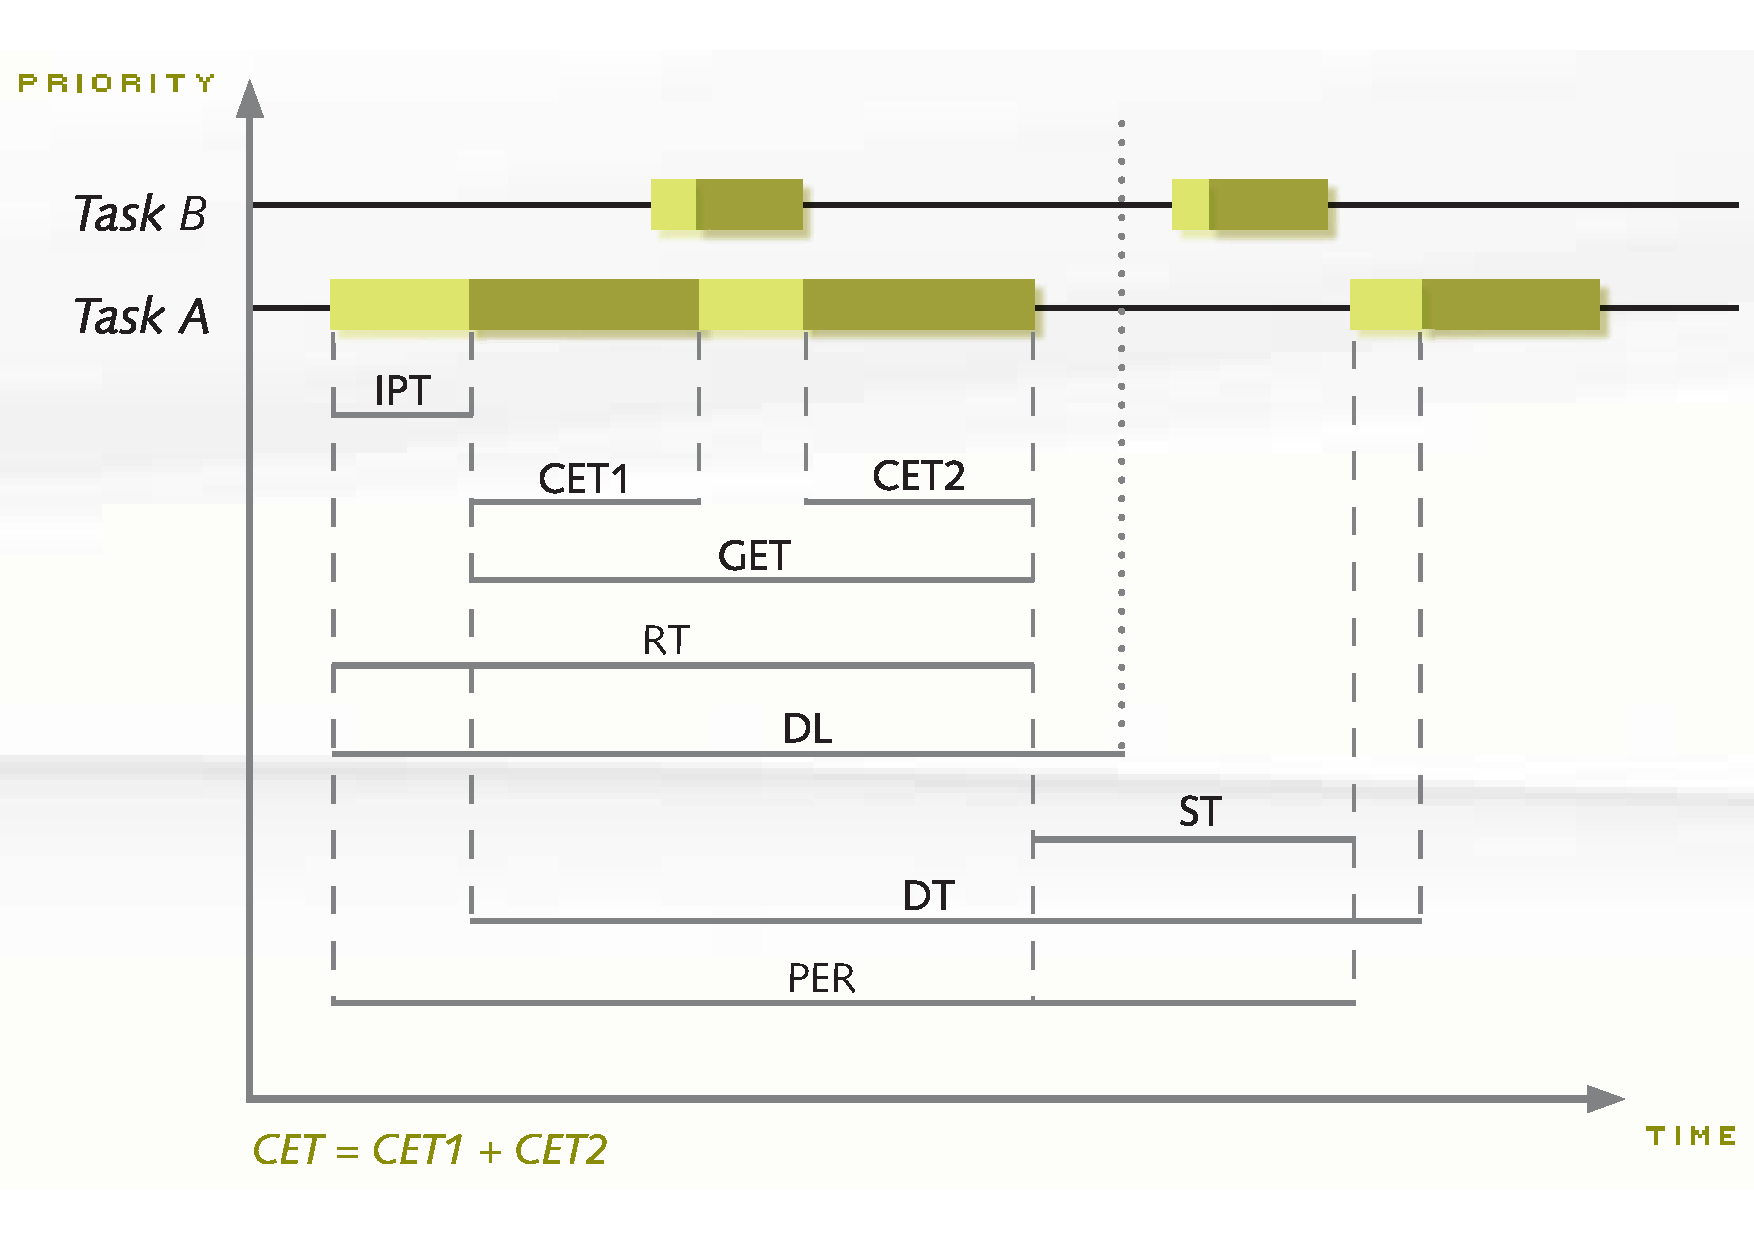
\includegraphics[width=\textwidth]{content/images/scheduling.pdf}
	\caption{Timing properties for scheduling in multi-tasked systems \cite{timingposter}}
	\label{fig:scheduling}
\end{figure}
\section{Real-time Parallelization Trends in Practice: RTOS, MPI, OpenMP, Pthreads, Java Threads} %x Give example of FreeRTOS for RTOS.
Some text will come here! \\
\section{Importance of Multi-core computing to automotive industry: AUTOSAR} %add autosar architecture picture
Some text will come here! \\
\begin{figure}[!ht]
	\centering
	\captionsetup{justification=centering}
	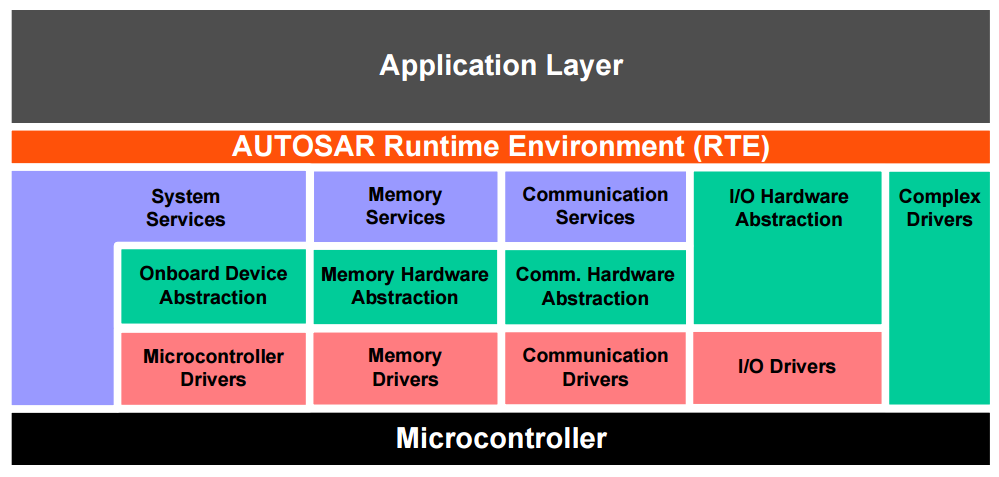
\includegraphics[scale=0.35]{content/images/autosararch.png}
	\caption{AUTOSAR Architecture \cite{autosararch}}
	\label{fig:autosararch}
\end{figure}
\section{Multi-core Programming with XMOS Multi-core Microcontrollers}
Some text will come here! \\
\section{Multi-core Programming with Raspberry Pi 3}
Some text will come here! \\
%%% CHAPTER Multi-core Programming ------------------end----
%%% CHAPTER APP4MC Development Environment ----------begin----
\chapter{APP4MC Development Environment}
\section{Introduction} %Motivation
\section{Features}
\section{Modeling}
%%% CHAPTER APP4MC Development Environment ------------end----
%%% CHAPTER A4MCAR ----------------------------------begin----
\chapter{Distributed Multi-core Demonstrator (A4MCAR) Design and Implementation}
\section{System Overview}
As introduced in the Introduction chapter, A4MCAR is a demonstrator RC-Car for the APP4MC development environment. A4MCAR provides a distributed multi-core architecture that allows the demonstration of embedded low-level and high-level applications. Pictures of the A4MCAR can be seen in Figure \ref{fig:a4mcar}.
\begin{figure}[!ht]
	\centering
	\captionsetup{justification=centering}
	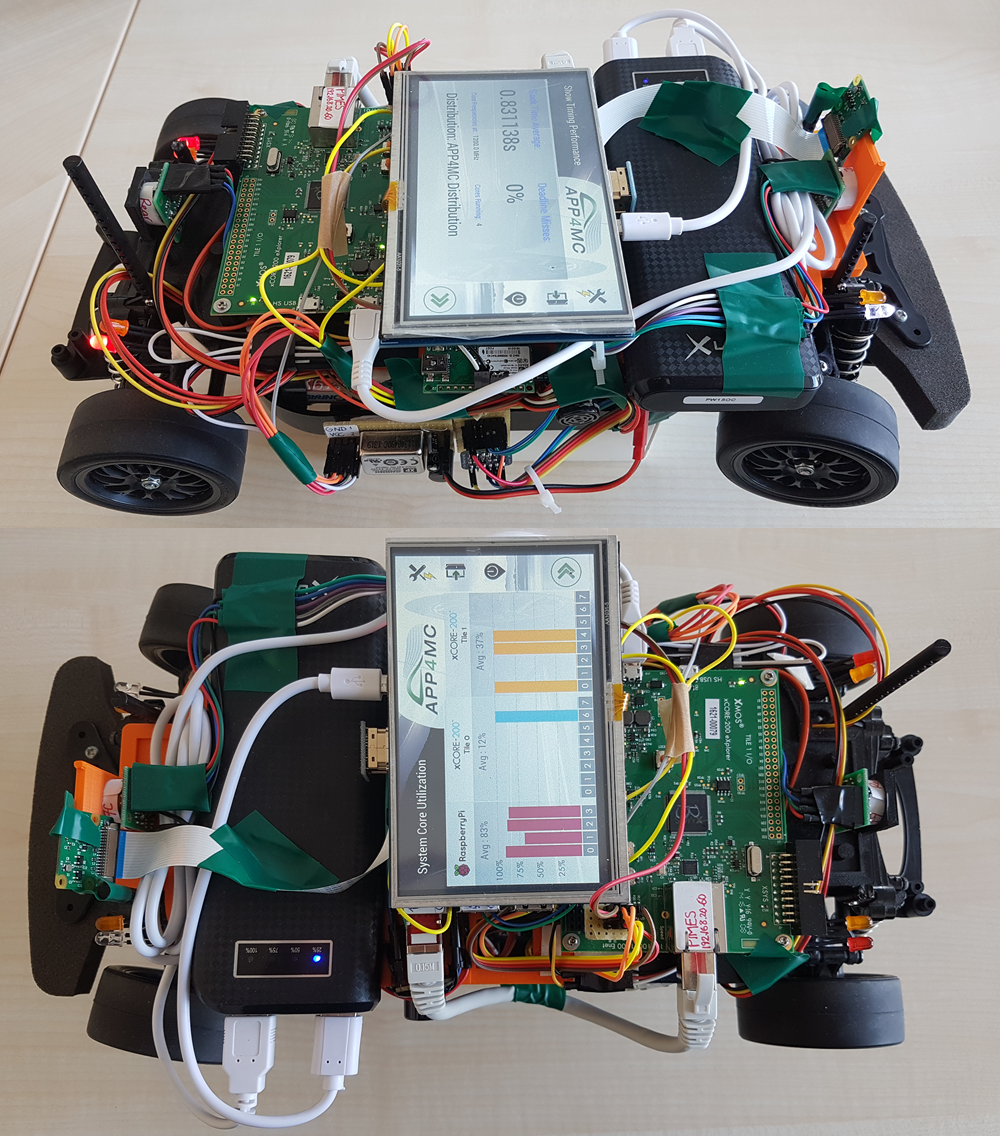
\includegraphics[scale=0.4]{content/images/a4mcar.png}
	\caption{A4MCAR}
	\label{fig:a4mcar}
\end{figure}
\subsection{System Features}
As A4MCAR targets automotive industry and parallelization studies done by APP4MC, it features not only sensing and actuation related features but also applications that would help with task to core distributions and parallelization performance evaluation. One could see the featured applications for the A4MCAR in Figure \ref{fig:tasksoverall}. 
\begin{figure}[!ht]
	\centering
	\captionsetup{justification=centering}
	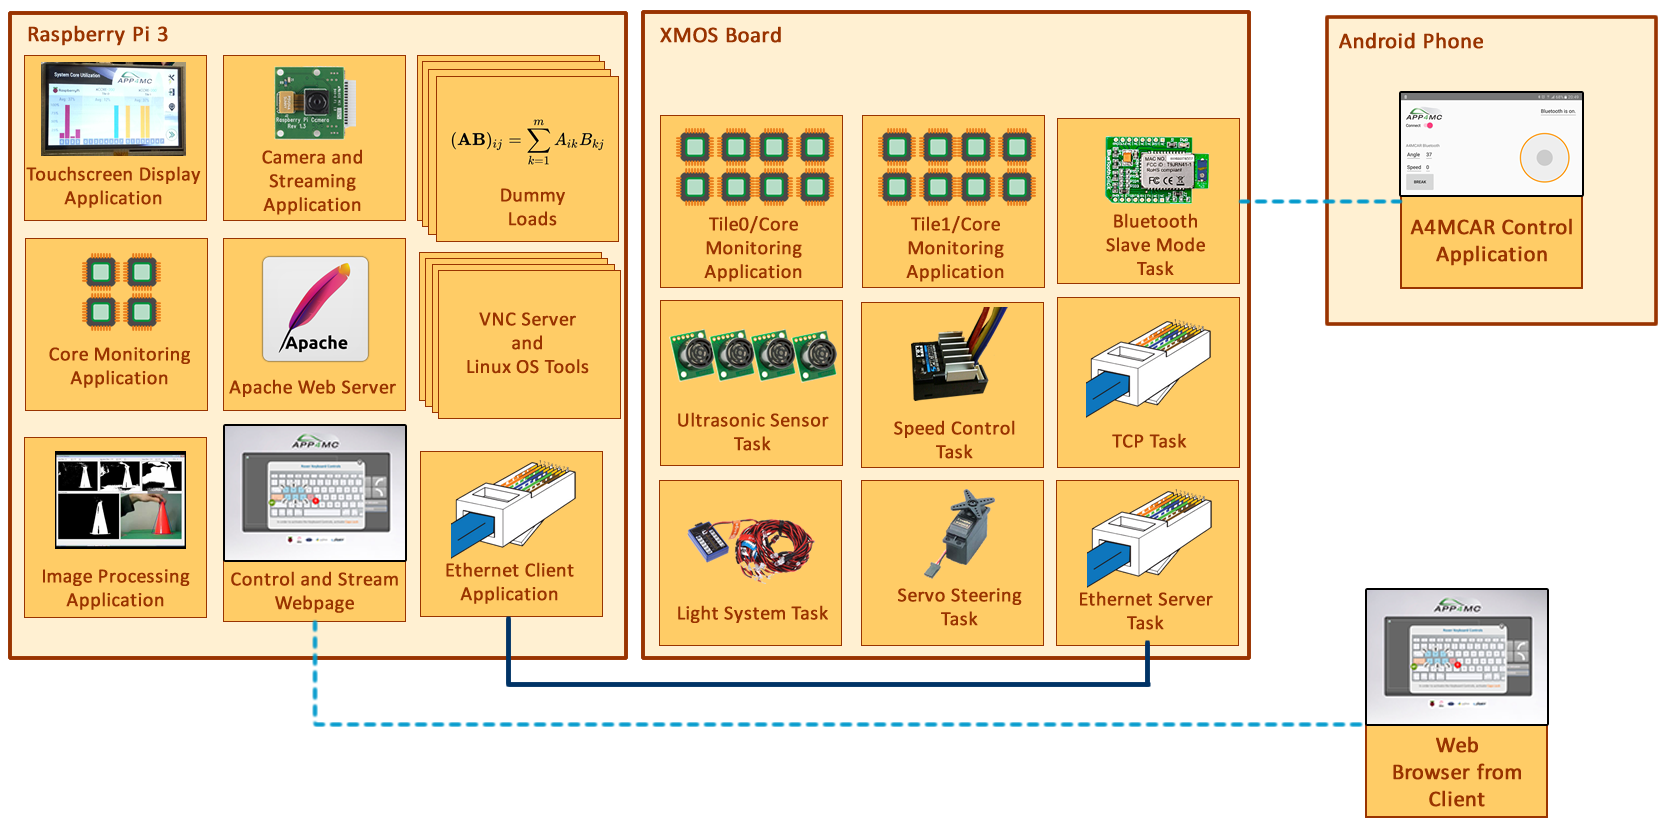
\includegraphics[scale=0.3]{content/images/tasksoverall.png}
	\caption{Applications developed and/or maintained for A4MCAR}
	\label{fig:tasksoverall}
\end{figure}
In the figure, it is seen that the low level module of A4MCAR, built using xCore-200 eXplorerKIT targets mostly actuation and sensing related applications. The full list of tasks developed for the low-level module includes:
\begin{itemize}
	\item Core monitoring applications for each tile (two exist) that calculates the average core usages.
	\item Bluetooth task to configure bluetooth module in slave mode and receive data over UART interface.
	\item Proximity measurement task that obtaines the distance sensor information from four SR-04 sensors over an I2C sensor network.
	\item Speed control task in order to use PWM to drive speed controlling motor.
	\item Steering task that controls a servo motor using PWM signaling in order to steer the A4MCAR using external inputs.
	\item Light system task in order to control a light module for certain conditions.
	\item Ethernet server task to maintain a TCP server for data reception and transmission from high level module.
	\item TCP task and several other ethernet configuration related tasks to configure ethernet module (PHY) drivers and establish proper TCP connection.
\end{itemize}
In order to investigate parallelization outcomes on Real-time Linux and make use of high level features such as web server, image processing and touchscreen interface high-level module is introduced to the system. High-level module is designed so that it can communicate with low-level module over TCP in order to send driving information and retrieve core information from low-level module. It is important to mention that high-level module uses Raspberry Pi 3 in order to achieve high level tasks using a robust Debian-based OS, namely Raspbian. Although the features of the high-level module is illustrated in the Figure \ref{fig:tasksoverall}, full feature list can be given as follows:
%xxxxxxxxxxxxxxxx
\begin{itemize}
	\item Core monitoring application that calculates the average core usages on each core.
	\item Image processing application that helps to find a traffic cone.
	\item Apache Web Server that is used to host a web page which shows average core usage, show Raspberry Pi 3 camera (Raspicam) stream and helps to drive the A4MCAR via web page controls.
	\item Ethernet client application that writes handles data transmission and reception to and from server using file operations and data parsing.
	\item Camera and streaming application that starts the Raspicam and maintains the stream using configuration parameters such as resolution, quality, frame rate, port and etc.
	\item A webpage which is used for driving the A4MCAR as well as display core usages on each core and Raspicam stream.
	\item A touchscreen display application which is used for displaying all cores and their utilization, starting and killing all applications on high-level module, allocation of processes on high-level module to cores dynamically, visualization of timing related performance indicators such as average slack time and deadline misses percentage, selecting different distributions, and configuration of the IP addresses on high-level module.
	\item Dummy load processes that perform random matrix multiplication in order to find performance indicators in full utilization.
	\item Several Linux processes that run Linux OS kernel and VNC server process that provides PC connection via SSH connection.
\end{itemize}
\subsection{Infrastructure}  %x XMOS and Rpi: boards, (inkl. board pictures) processors, memory, languages, compilers, infrastructure
Processing infrastructure of the A4MCAR is divided into two modules: Low-level module and high-level module. Low-level module uses a multi-core development kit XMOS xCore-200 eXplorerKIT, whereas high-level module uses a Raspberry Pi 3 which are both shown in Figure \ref{fig:boards}.
\begin{figure}[!ht]
	\centering
	\captionsetup{justification=centering}
	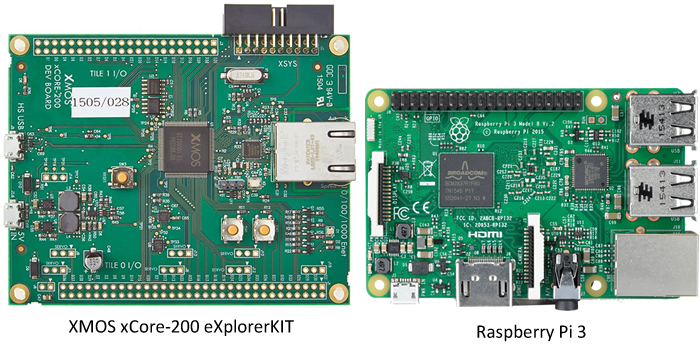
\includegraphics[scale=0.6]{content/images/boards.jpg}
	\caption{Development boards used in A4MCAR}
	\label{fig:boards}
\end{figure}

\subsubsection{Low-level Infrastructure}
XMOS xCore-200 eXplorerKIT features XEF216-512, a powerful multi-core microcontroller that provides sixteen 32-bit logical cores that are divided into tiles \cite{xmoskitweb}, which are identical units that contain processing unit, cache memory and switch mechanism \cite{tileref}. XMOS xCore-200 eXplorerKIT contains two tiles with eight logical cores in each tile. It is important to add that logical cores of eXplorerKIT provides 2000 MIPS (Million Instructions per Second) processing power and 512 KB SRAM along with up to 500 MHz clock speed. The specified performance values are considered to be relatively powerful compared to regular microcontrollers. While the processing power and cache memory of its two tiles are identical, ports on each tile have access to different peripherals located on the board. With 53 high-performance GPIO, XMOS xCore-200 eXplorerKIT features 100/1000Mbps Ethernet module, high speed USB interface, a 3D accelerometer, a 3-axis gyroscope, and six servo interfaces which makes the kit useful in a wide variety of applications that include robotics, automotive, signal processing and communication applications \cite{xmoskitweb}.

As the name of the development kit suggests, XEF216-512 uses XMOS' xCore-200 architecture. An illustration of xCore-200 architecture is given in Figure \ref{fig:XE216Architecture}.
\begin{figure}[!ht]
	\centering
	\captionsetup{justification=centering}
	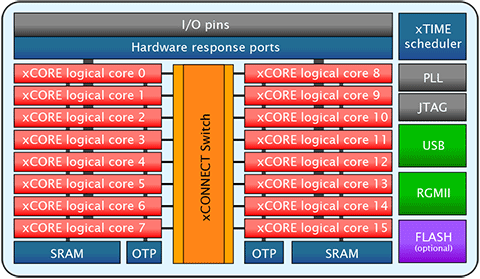
\includegraphics[scale=0.7]{content/images/XE216Architecture.png}
	\caption{Illustration of XMOS' xCore-200 Architecture \cite{xmosflyer}}
	\label{fig:XE216Architecture}
\end{figure}

In xCORE-200 architecture, each core uses the memory of the tile it belongs to and logical cores communicate using a high-speed network. Thus, channels which achieve task communication are linked to other cores via \textbf{xCONNECT Switch}. While this is the case for tasks that are distributed to seperate cores, for tasks that are placed in the same core \textbf{xTIME Scheduler} automatically schedules tasks by synchronizing events. The xTIME Scheduler works similar to RTOS in traditional microcontrollers and uses \textbf{Round-robin scheduling method} \cite{xmosdatasheet} \cite{roundrobin} which is a simple and starvation-free scheduling technique that gives each task equal time slices and disregards priorities in order to schedule processes or tasks. Round-robin scheduling is widely used in operating systems \cite{roundrobin}.

In xCORE architecture, the synchronization of task communication is handled by events rather than ISRs (Interrupt Service Routines) as compared to a traditional microcontroller. Each xCORE tile is connected to hardware ports and thereby pins which can be driven high and low in order to drive electrical peripherals. xCORE tiles are also connected to an OTP (One Time Programmable Memory) and SRAM (Static Random Access Memory). While OTP is used for code locking features, SRAM serves as a memory where the instructions and variables are located \cite{xmosdatasheet}.

Since the xCORE features multiple cores unlike a traditional microcontroller, it should be clearly understood that the task interruption is not present in xCORE. This is illustrated delicately in the Figure \ref{fig:xmosvstraditional} \cite{xmosflyer}. If not stated otherwise in an xCORE application, all the tasks are placed to different logical cores. This means that all the tasks are executed completely parallel in hardware. When the tasks are shared in a core, then the multi-tasking features of the XMOS are invoked and parallelized just like in an RTOS from traditional microcontrollers \cite{xmosflyer}.
\begin{figure}[!ht]
	\centering
	\captionsetup{justification=centering}
	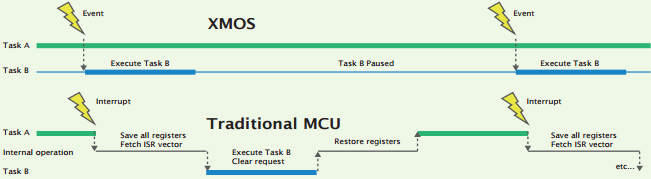
\includegraphics[width=\textwidth]{content/images/xmosvstraditional.png}
	\caption{XMOS vs Traditional Microcontroller \cite{xmosflyer}}
	\label{fig:xmosvstraditional}
\end{figure}

Most of the traditional microcontrollers including xCORE microcontrollers nowadays feature pipelining mechanism. The \textbf{instruction pipeline} is a set of data processing elements connected in series, where the output of one element is the input of the next one \cite{pipelinebook}. Via instruction pipelining, processors make use of the stages in order to use the clock to its full performance to reduce the time taken to execute instructions. This mechanism is also present in most of the XMOS processors with five stages. How instruction pipelining mechanism achieves faster instruction execution is illustrated in the Figure \ref{fig:pipeline} \cite{xmosflyer}.
\begin{figure}[!ht]
	\centering
	\captionsetup{justification=centering}
	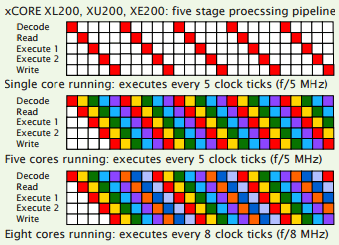
\includegraphics[scale=0.9]{content/images/pipeline.png}
	\caption{Pipelining Explained on XMOS \cite{xmosflyer}}
	\label{fig:pipeline}
\end{figure}

Traditionally, XMOS based microcontrollers are programmed via xTimeComposer, which is an Eclipse-based software development platform for XMOS based multi core microcontrollers with integrated features such as simulation, symbolic debugging, tracing, runtime instrumentation, and timing analysis with a static code timing analyzer called \textbf{XTA}\cite{xmosflyer}. As A4MCAR needs to make use of timing and performance values, some tracing tools and XTA has been widely used during the development. xTIMEComposer development environment windows are shown and illustrated in Figure \ref{fig:xtimecomposerwindows}.
\begin{figure}[!ht]
	\centering
	\captionsetup{justification=centering}
	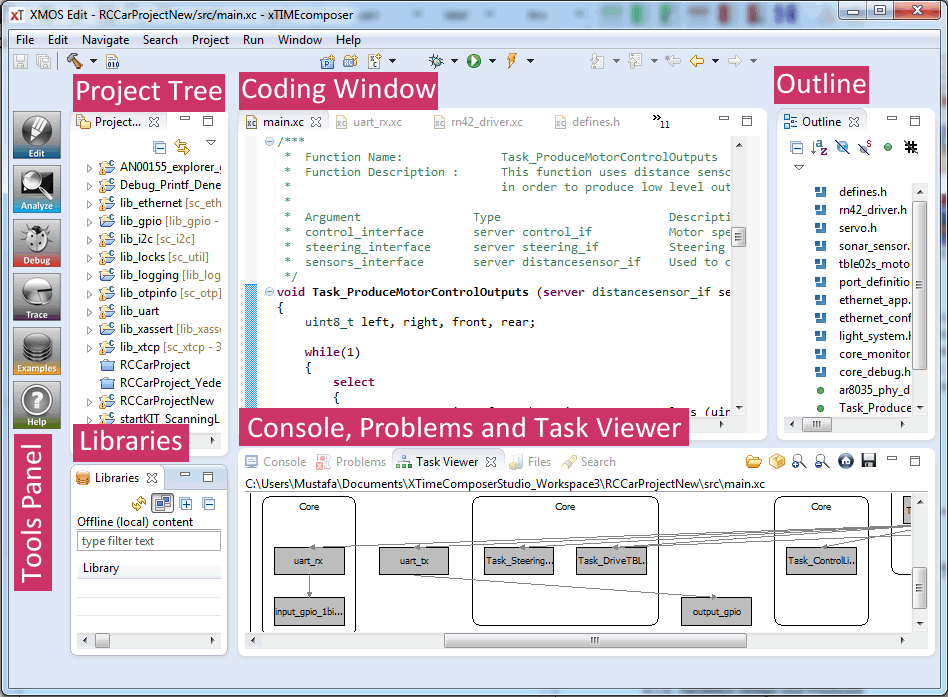
\includegraphics[scale=0.5]{content/images/xtimecomposerwindows.png}
	\caption{xTIMEComposer 14.2.3 Development Environment Windows}
	\label{fig:xtimecomposerwindows}
\end{figure} \\
%Explain the fucking composer
In the Figure \ref{fig:xtimecomposerwindows} it is seen that the main development environment consists of the following windows:
\begin{itemize}
	\item \textbf{Project Tree:} This window is used for managing projects and source, include, binary and configuration files within projects.
	\item \textbf{Coding Window:} Coding window is used for writing code and placing breakpoints. One can switch between several files by clicking on the tabs located on the top of this window.
	\item \textbf{Console:} The console is used for viewing the building process, verbose and debugging information.
	\item \textbf{Problems:} The problems window is used for seeing warnings and errors that result from the code.
	\item \textbf{Task Viewer:} The task viewer is a special feature that is unique in xTIMEComposer and it is used to visualize tasks and at which core and tile they are located. The channel and interface connections between tasks are also visualized using this window.
	\item \textbf{Tools Panel:} This window is used in order to switch between several tools that xTIMEComposer provide. Analyze and Debug tools are widely used in development. Analyze tool opens xTIMEComposer Timing Analyzer (XTA) tool whereas Debug tool is used for traditional debugging using breakpoints.
	\item \textbf{Outline:} Outline window lays out the main elements of a file such as its includes, tasks, objects and so on.
	\item \textbf{Libraries:} The Libraries window can be used in order to search offline and online libraries.
\end{itemize}
%files in a project.. configuration..
%\begin{figure}[!ht]
%	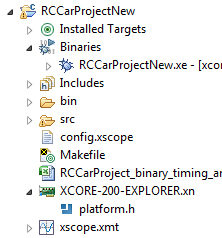
\includegraphics[scale=0.9]{content/images/xtimeprojecttree.jpg}
%	\caption{Files in a xTIMEComposer project}
%	\label{fig:xtimeprojecttree}
%\end{figure}
%languages
Programming languages which are used for xCORE processors can be listed as C, C++ and xC (C with multicore extensions) \cite{xmosdatasheet}. The aforementioned xC language features three main keywords in order to represent task communication. To represent an interface that sends data to another task, \textbf{client} keyword is used whereas if a task is retrieving data from one or many client ports, the receiving interface is named \textbf{server}. It is important to mention that server interface receives data by throwing events. Additionally, xC also allows to define function attributes which are \textbf{combinable} and \textbf{distributable}. XMOS Programming Guide \cite{xmosprogrguide} suggests that combinable tasks are the ones that continuously react to events and they can be combined to have several tasks running on the same logical core. It is added in the XMOS Programming Guide \cite{xmosprogrguide} that distributable tasks are not dedicated to only one logical core but they run when required by the tasks connected to them. Furthermore, xC features \textbf{timers}, \textbf{events}, \textbf{guards}, \textbf{event priority ordering} in order to help us develop event-based software. These features of xC make multi-core programming easy and robust on xCORE processors.

\subsubsection{High-level Infrastructure}
%xxxxxxxxxxxxxxxx
High-level processing unit of A4MCAR, Raspberry Pi 3, is a widely used single board computer in embedded applications. It has 1.2GHz 64-bit quad-core processor with ARMv8 architecture, 1GB of RAM, VideoCore IV 3D graphics core and several interfaces such as 40 GPIO pins, 4 USB ports, HDMI port, ethernet port, audio jack, camera interface (CSI), display interface (DSI), micro SD card slot \cite{raspberrypiinfo}. The reason Raspberry Pi 3 is preferred in embedded systems applications is that it provides excellent connectivity via 802.11n Wireless LAN module, Bluetooth 4.1 module, and Bluetooth Low Energy (BLE) module. 

Raspberry Pi 3 can be booted with modern Linux-based operating system distributions such as Debian-based Raspbian OS \cite{raspbiandownload} and Ubuntu-based Ubuntu MATE\cite{ubuntumatedownload} \cite{raspberrypiinfo}. It should be noted that in A4MCAR, Raspbian OS has been used due to its wide software repository and driver support. The fact that Raspberry Pi 3 functions as a Linux computer helps in developing high-level applications that require operating system presence. The open-source nature of Linux and its software ecosystem provides flexible and traceable software development. In A4MCAR, the traceability and flexibility features of Raspberry Pi 3 are highly used. Furthermore, a wide variety of programming languages such as C, C++, Java, LISP, Python, Bash, Perl etc. are supported in Raspberry Pi. In A4MCAR, programming languages such as C, C++, Python, Bash, HTML, JavaScript has been used in order to develop high-level module.

A brief explanation of the architecture of Linux-based computers and as an extension the architecture of the Raspberry Pi 3 should be given in order to develop applications and understand how applications running on Linux work. With that idea in mind, high-level overview of the structure of  the \textbf{Linux kernel} and high-level layers in a Linux system which is given in Figure \ref{fig:linuxarchitecture} should be considered \cite{linuxkernelbook}.
\begin{figure}[!ht]
	\centering
	\captionsetup{justification=centering}
	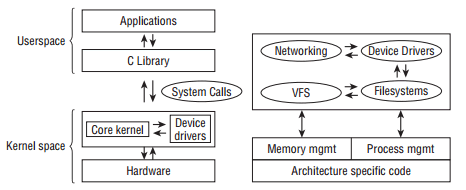
\includegraphics[scale=0.9]{content/images/linuxarchitecture.png}
	\caption{High-level Linux system architecture \cite{linuxkernelbook}}
	\label{fig:linuxarchitecture}
\end{figure}

According to Mauerer \cite{linuxkernelbook}, the kernel is the intermediary level between the hardware and the software that addresses the devices and the components of the system (such as CPU, memory and I/O devices) by passing application requests. While kernel processes requests from user applications, it makes its own decision where data is located and which commands to send to hardware. Kernel is also the instance in a Linux system which shares available resources such as CPU, memory, and network; which is why it should be addressed while working with parallel applications.

In the figure, it is seen that kernel space is not only responsible for accessing device drivers, but it is also responsible for memory and process management. A program under Unix systems (such as Linux) that run continuously is referred to as \textbf{processes} and they are scheduled by Linux kernel. The multi-tasking of processes are done by a mechanism that is called \textbf{task-switching} or \textbf{context-switching} and this is achieved to ensure that CPU performs according to the scheduled tasks. The concept of \textbf{scheduling} in a Linux system is also handled by kernel and it is the procedure of deciding how CPU time should be shared between existing processes. Additionally, \textbf{threads} in a Linux-based computer system are also big parts of multi-tasking which are also handled by kernel. Threads share the same data and resources but they have different execution paths through program \cite{linuxkernelbook}.

In A4MCAR high-level module, we mostly deal with processes and investigate ways to efficiently parallelize process-based system. In this regard, it is crucial to understand the process life cycle and how kernel schedules processes. This knowledge is described delicately by Mauerer \cite{linuxkernelbook} and Ward \cite{howlinuxworksbook}. Figure in \ref{fig:processlifecycle} depicts an illustration of how process life cycle works \cite{linuxkernelbook}.
\begin{figure}[!ht]
	\centering
	\captionsetup{justification=centering}
	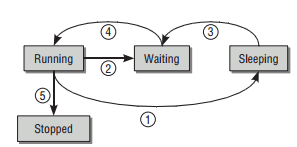
\includegraphics[scale=1]{content/images/processlifecycle.png}
	\caption{Process Life Cycle in a Linux System \cite{linuxkernelbook}}
	\label{fig:processlifecycle}
\end{figure}

% process life cycle explain..
In Figure \ref{fig:processlifecycle}, state machine for processes in a Linux system is given. The states of processes can be listed as Running, Waiting, Sleeping, and Stopped. These states can be explained using following scenerios \cite{linuxkernelbook}:
\begin{itemize}
	\item If the process is being currently executed, process is in \textbf{Running} state.
	\item If the process is not being executed because it is waiting for CPU to finish executing another process, it is in \textbf{Waiting} state.
	\item If the process is waiting for an external event such as a periodic activation or a sporadic activation, it is in \textbf{Sleeping} state. Notice that transition from Sleeping state to Running state is not possible. A process switches to Waiting state from Sleeping state in order to wait for current process to finish its execution.
	\item If the user decides to kill (terminate) the application, the process goes into \textbf{Stopped} state.
	\item If a process has been killed but its entries are still alive in the process table, the state of that process is called \textbf{Zombie}. Therefore, although not shown, transition from Running state to Zombie state is also possible.
\end{itemize}

It is important to note that these states are traceable using Linux kernel access methods which will be explained in Section 5: "Information Tracing and System Management" of this report along with several other Linux kernel concepts.

% terminal, compilers, Nano, Vi, Emacs
Raspberry Pi is conventionally programmed through Linux shell which is programmed and commanded with the help of Bash scripting language. There are several editors and compilers introduced for Linux shell in order to help developers write, compile, debug, and trace their applications. Most popular editors involve Nano, Vi, and Emacs which are editors that can run without GNU Graphical User Interface. An alternative way is to use open-source platforms such as Eclipse with correct extensions and plugins. The conventional and standart C compiler for the Unix platform GCC, and the standart Python shell can be accessed using all these compilers. For the sake of demonstration, the Linux shell which is running Emacs is shown in the Figure \ref{fig:linuxeditors}. It is important to note that in the development of A4MCAR, Nano and Emacs editors have been frequently used as Nano provides easiest way to interact with Linux shell and Emacs provides advanced features to compile and debug programs rapidly.
\begin{figure}[!ht]
	\centering
	\captionsetup{justification=centering}
	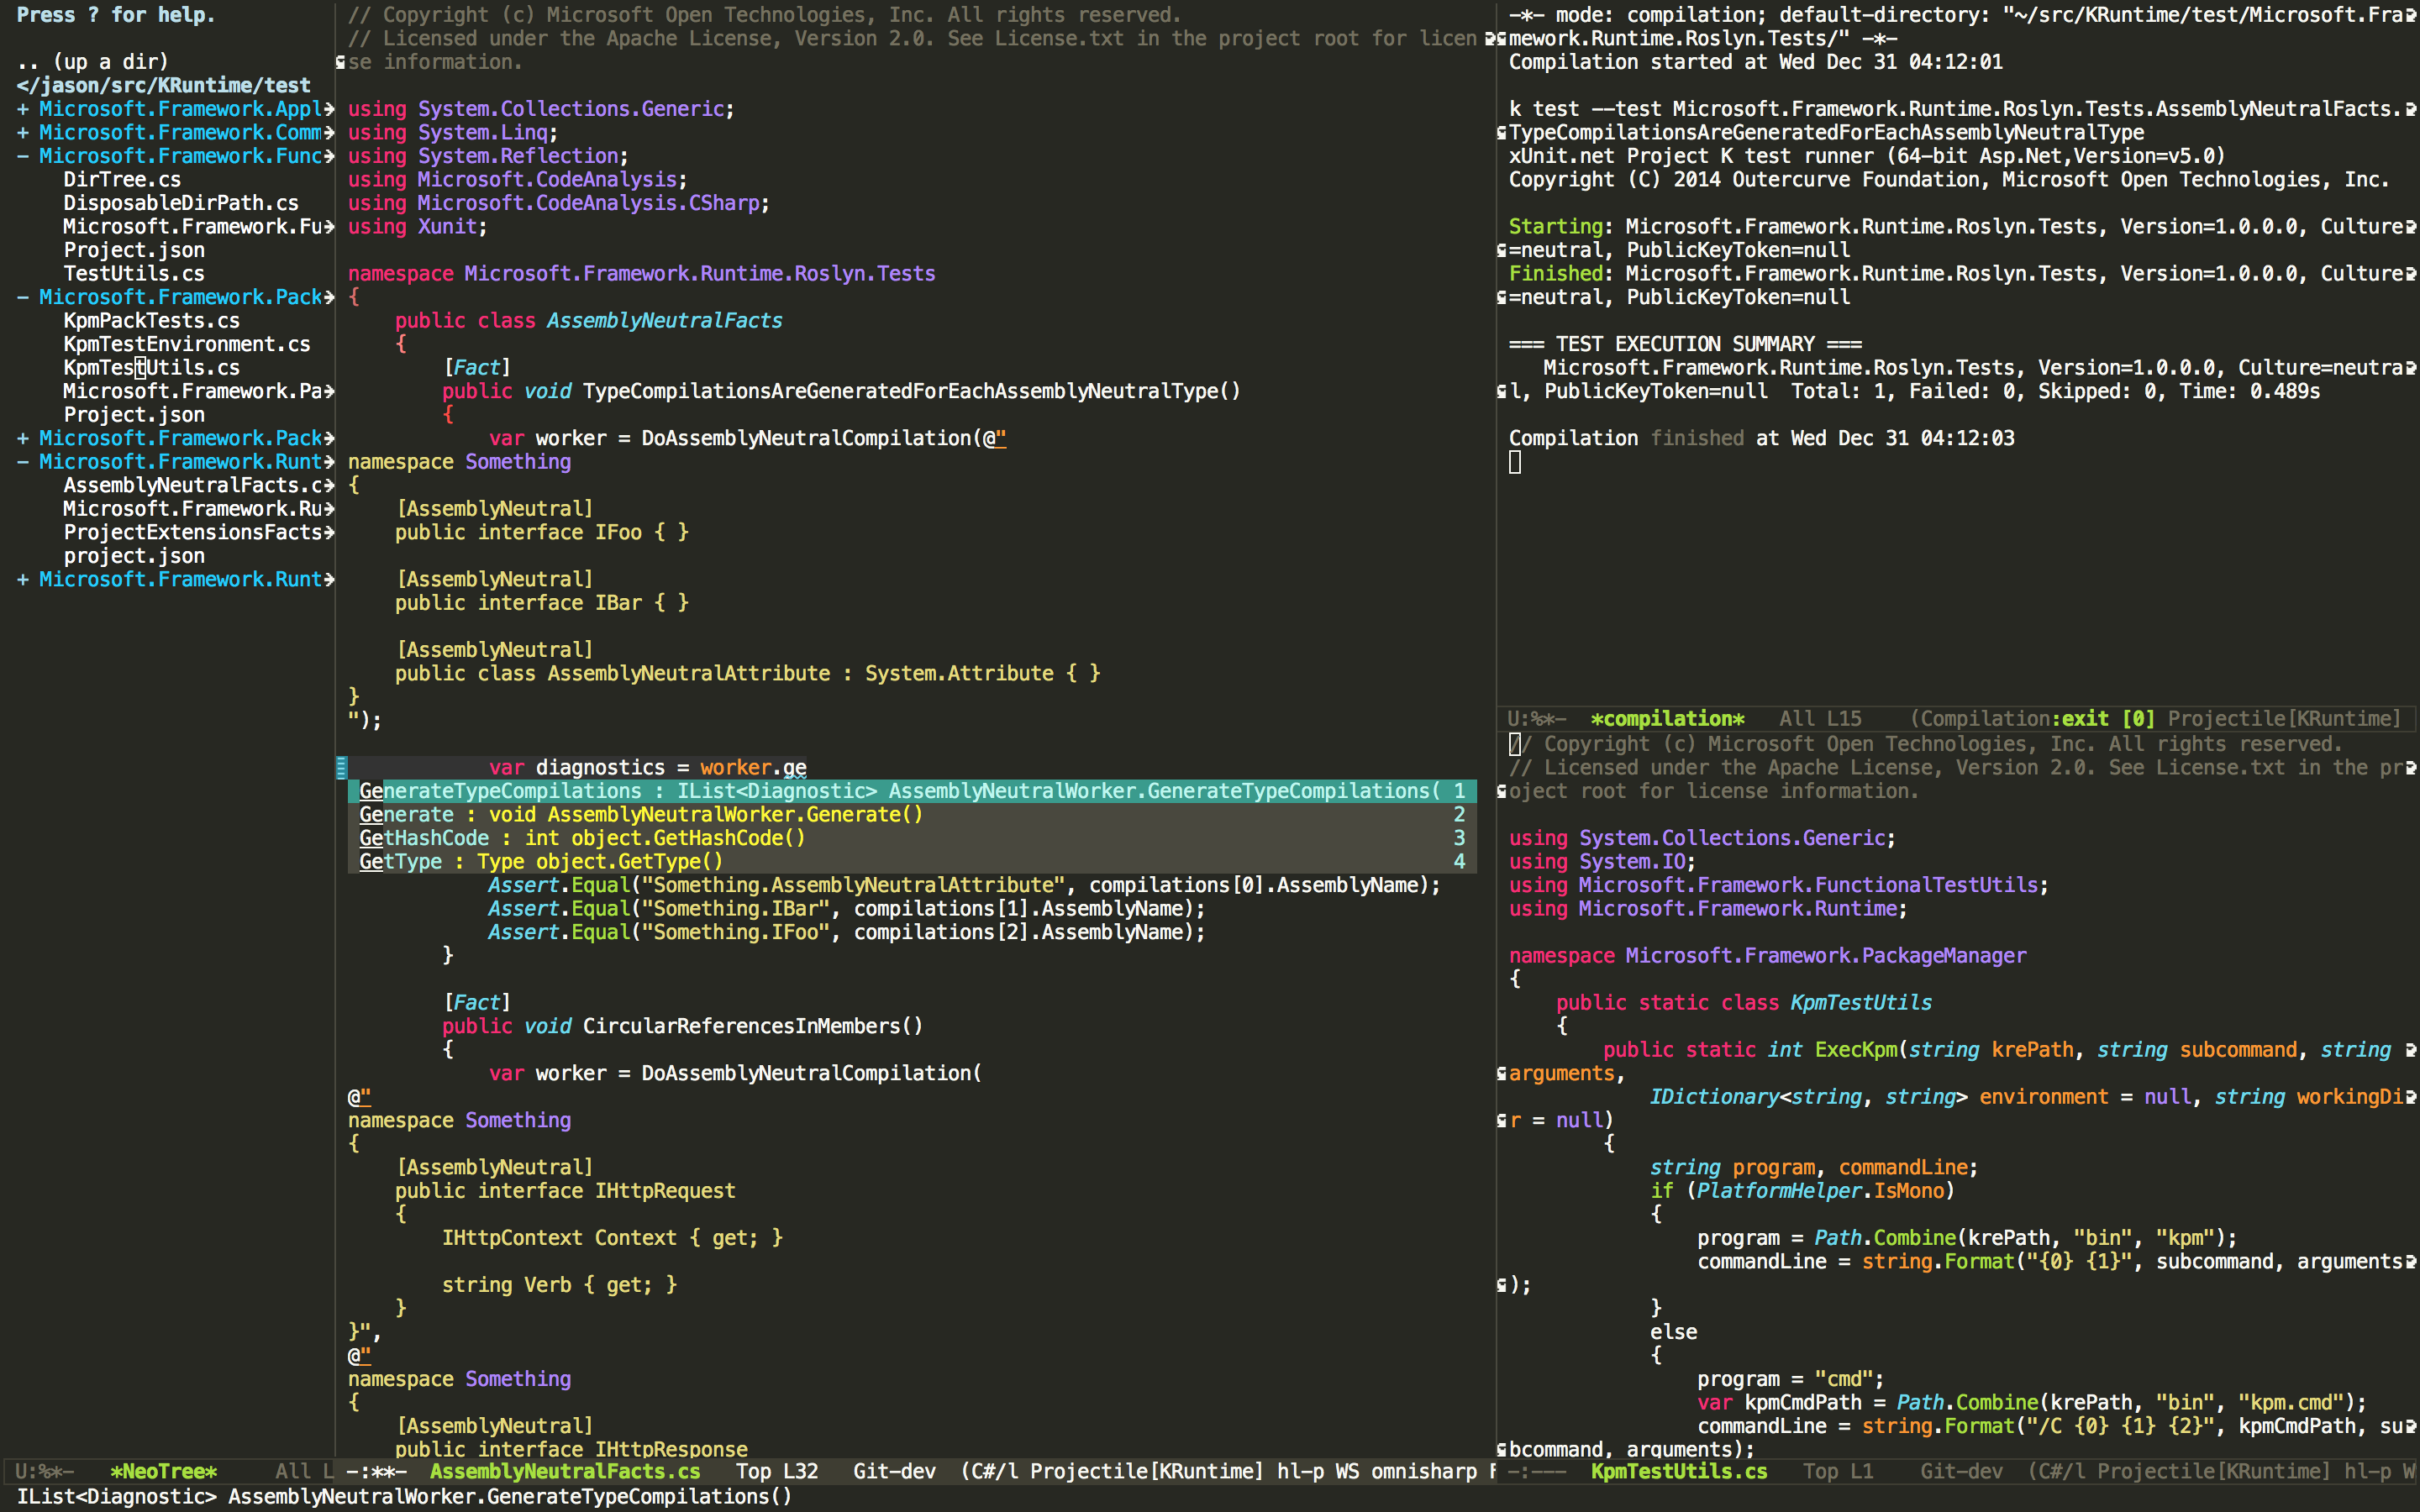
\includegraphics[scale=0.26]{content/images/linuxeditors.png}
	\caption{Linux Shell running Emacs}
	\label{fig:linuxeditors}
\end{figure}
%Raspbery Pi stuff here!
\subsection{Hardware Design, Sensors and Protocols}
One should care for a robust hardware design in order to avoid having software problem and safety related issues. In A4MCAR, a number of modules have been used alongside development kits in order to provide utility to the demonstrator. On the low-level module side, a light system, an RN-42 Bluetooth module, four SRF-02 ultrasonic sensors, a servo motor, a TBLE-02S electronic speed controller have been used. The high-level module side however only is connected to a touchscreen display and a Raspicam (Raspberry Pi camera). The overview of hardware connections, used protocols and device architectures are given in the Figure \ref{fig:hwoverview}.
\begin{figure}[!ht]
	\centering
	\captionsetup{justification=centering}
	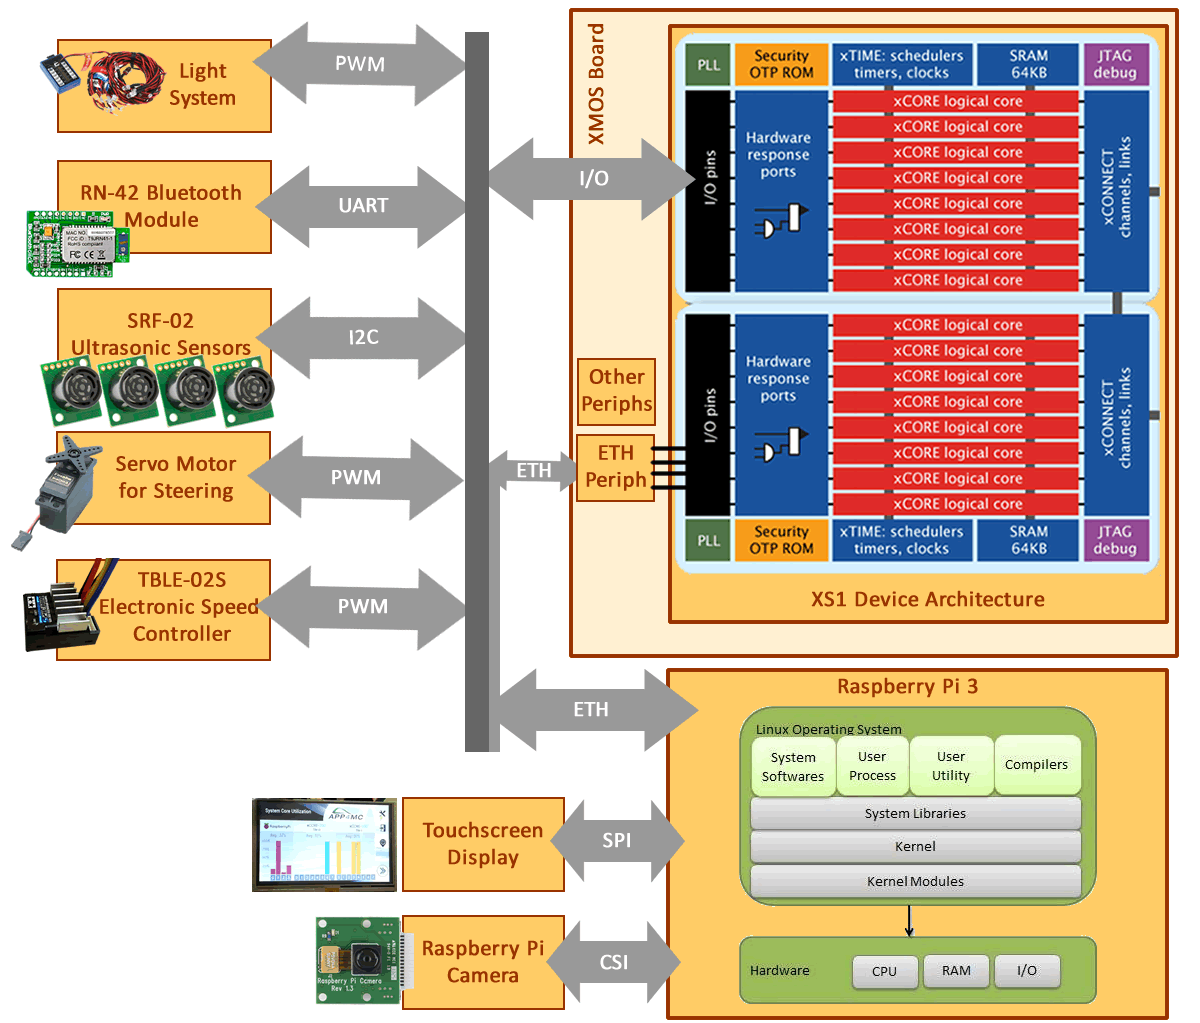
\includegraphics[width=\textwidth]{content/images/hwoverview.png}
	\caption{Hardware overview of A4MCAR}
	\label{fig:hwoverview}
\end{figure}

The system uses various communication protocols, seen in Figure \ref{fig:hwoverview} in order to interact with sensors, actuators and utility devices. The communication protocols and associated devices used in A4MCAR could be listed as follows:
\begin{itemize}
	\item \textbf{PWM:} In order to interact with servo motor, TBLE-02S electronic speed controller, and light system, Pulse Width Modulation (PWM) have been used. PWM is a type of modulated digital signal used mostly in control applications \cite{pwm}. By describing how much a signal is high and low with respect to time, duty cycle is measured which is given in percentage. One could observe the signal illustration given in \ref{fig:pwm} to see how commonly used duty cycles look like. In a control circuitry, by achieving various duty cycles, dimming a light or controlling the direction or speed of a motor is possible \cite{pwm}.
	\begin{figure}[!ht]
		\centering
		\captionsetup{justification=centering}
		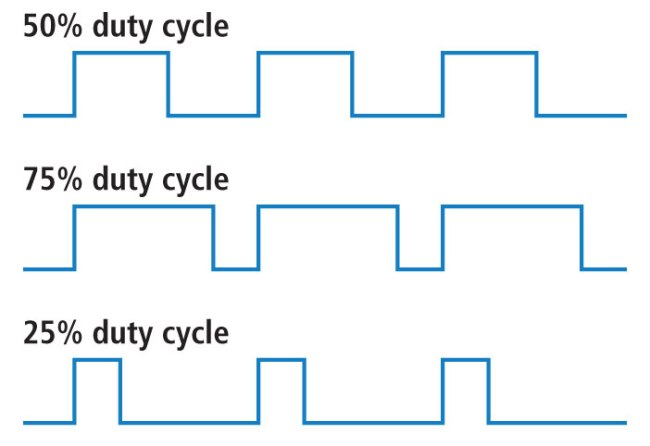
\includegraphics[scale=0.5]{content/images/pwm.jpg}
		\caption{Duty cycle example in pulse width modulation \cite{pwm}}
		\label{fig:pwm}
	\end{figure}
	\item \textbf{UART:} The RN-42 is a master-slave configurable bluetooth module (shown in Figure \ref{fig:hwoverview}) that is programmed using AT commands via UART. In A4MCAR, a RN-42 bluetooth module is used in order to interact with the bluetooth of Android devices. UART (Universal Asynchronous Receiver and Transmitter) is a communication protocol that achieves simple communication of two equivalent nodes. UART is a half-duplex and asynchronous serial protocol that doesn't communicate using a clock. Half-duplex nature of UART makes it so that transmitting and receiving lines can not be achieved simultaneously. It became a universal format because it is being used in telephone lines and USB ports of computers for decades. Number of bits transmitted or received per second is referred to as baud rate and it is standardized to values such as 9600, 14400, 19200, 38400, 57600, and 115200. Basic UART data packet is given in Figure \ref{fig:uartpacket}. The figure should depict that the basic format usually contains 6 to 8 data bits and start and stop bits to mark start and stop of the data packet. It should be noted that there are various formats with different sizes \cite{uart}.
	\begin{figure}[!ht]
		\centering
		\captionsetup{justification=centering}
		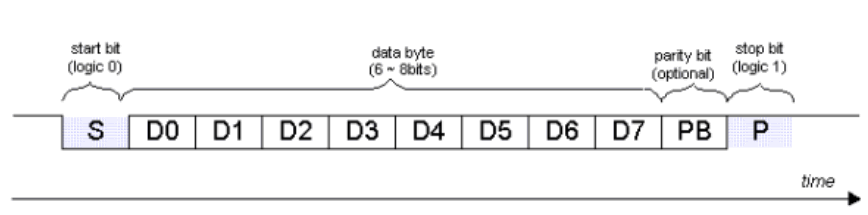
\includegraphics[scale=0.5]{content/images/uartpacket.png}
		\caption{Simple UART data packet \cite{uart}}
		\label{fig:uartpacket}
	\end{figure}
	\item \textbf{I\textsuperscript{2}C:} The proximity sensor network of A4MCAR that consists of four SRF-02 sonar sensors uses I\textsuperscript{2}C communication protocol in order to address devices in the network and obtain distance information in centimeters. I\textsuperscript{2}C (Inter integrated circuit) is a communication protocol that is intended for short distance that handles the communication of multiple slave units with one or multiple master units. Its advantage is that it uses only two wires in order to handle communication between many devices. Compared to the very similar serial communication protocol SPI, I\textsuperscript{2}C can support a multi-master system with up to 1008 slave devices. I\textsuperscript{2}C chips consist of two signals: clock signal SCL and data signal SDA. Since signals are open drain, each signal must have a pull-up resistor. The communication is handled by sending the address of the register and the data to be sent in order to write into the registers of the I\textsuperscript{2}C chips. A basic frame with 7 address bits and 8 data bits is given in \ref{fig:i2cframe} \cite{i2c}.
	\begin{figure}[!ht]
		\centering
		\captionsetup{justification=centering}
		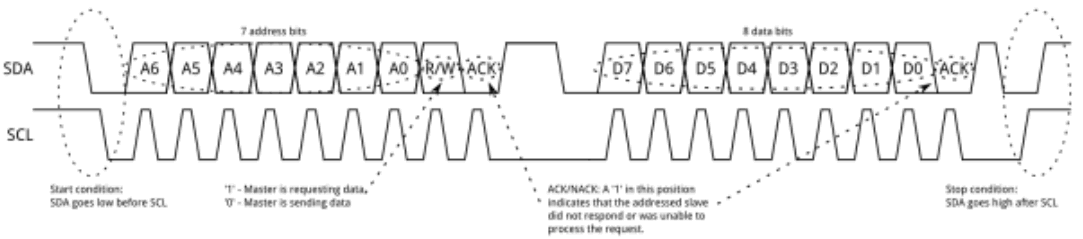
\includegraphics[scale=0.4]{content/images/i2cframe.png}
		\caption{I2C protocol frame\cite{i2c}}
		\label{fig:i2cframe}
	\end{figure}
	\item \textbf{Ethernet/TCP}: Ethernet communication using TCP (Transmission Control Protocol) is a very common method of communation that is applied within the Application, Presentation, and Session layers of the well-known OSI model. It is also a protocol that is used for high-speed data transmission to other network devices on the same network segment if used in Telnet mode. Ethernet defines two units of transmission, packet and frame. The frame includes not just the "payload" of data being transmitted but also addressing information identifying the physical "Media Access Control" (MAC) addresses of both sender and receiver, VLAN tagging and quality of service information, and error-correction information to detect problems in transmission \cite{ethernet1} \cite{ethernet2}. 
	
	In A4MCAR, a telnet server and client has been implemented using TCP protocol in order to send and receive data between high-level and low-level modules. The high-level module is configured as client, whereas low-level module is configured as the server. 
	\item \textbf{SPI}: Just like I\textsuperscript{2}C, SPI (Serial Peripheral Interface) is a communication protocol that is used to send data between processors and small devices such as sensors and displays. In SPI, MOSI, MISO, and SCK lines are available that are two data lines for each direction and a clock line. Additionally, a line of SS (Slave Select) could be used in order to select which slave device in the network is being addressd at that moment. Since SPI does only work with clock unlike the conventional UART, SPI is a synchronous communication method \cite{spi}.
	
	In A4MCAR, SPI is used by touchscreen kernel drivers in order to get touchscreen controls working. HDMI interface is also used in order to transfer media from Raspberry Pi to the Touchscreen Display.
	\item \textbf{CSI}: CSI (Camera Interface) is used by third-party applications and it is the interface that is used in order to get RaspiCam working.
\end{itemize}

In the Figure \ref{fig:RCCAR_Schematics}, the complete circuit schematics regarding A4MCAR low-level module is given. Interfacing sensors and devices should be done accordingly in order to program peripherals with xCORE-200 board properly. 
\begin{figure}[!ht]
	\centering
	\captionsetup{justification=centering}
	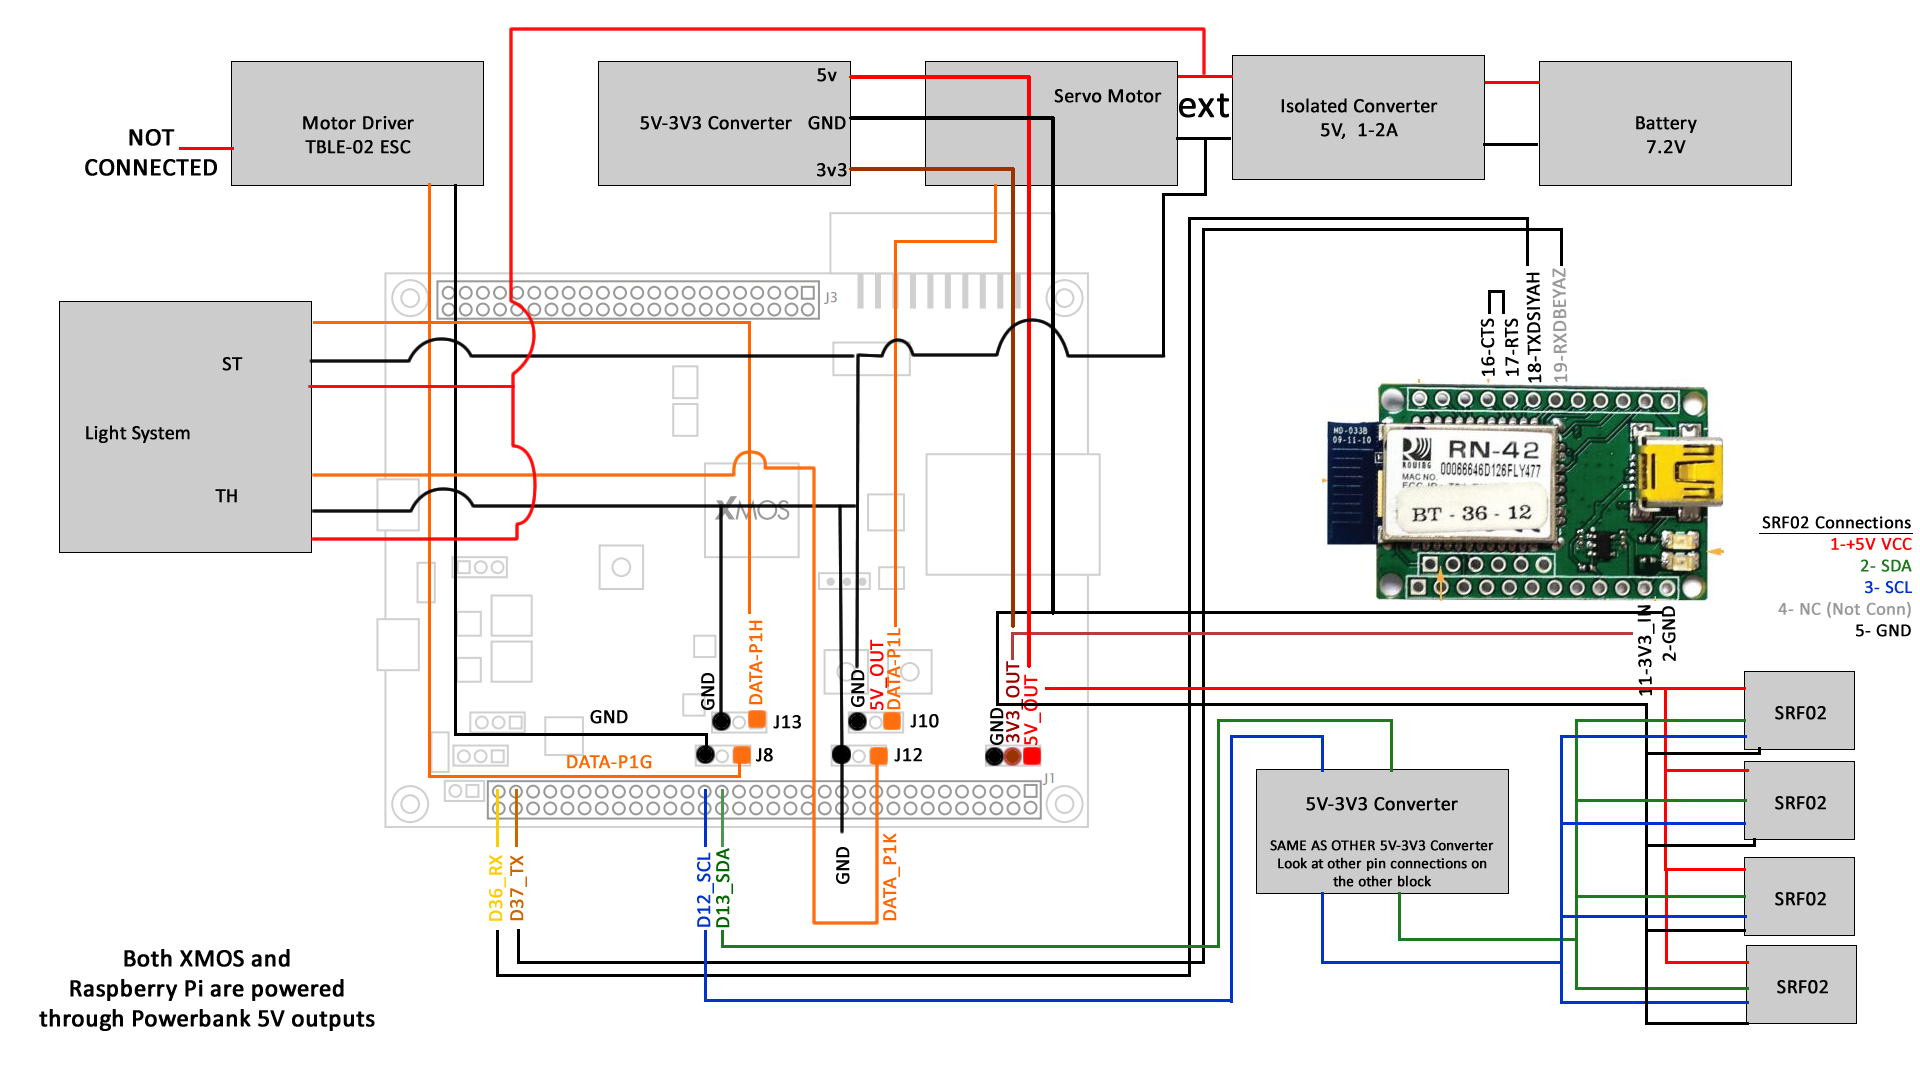
\includegraphics[width=\textwidth]{content/images/RCCAR_Schematics.png}
	\caption{Low-level module schematics of A4MCAR using XMOS xCore-200 eXplorerKIT}
	\label{fig:RCCAR_Schematics}
\end{figure}
\subsection{Safety and Power}
It should be noticed in the Figure \ref{fig:RCCAR_Schematics} there are three units that are introduced in order to get rid of the problems that are related to safety and power. To start with, since it is stated in the XS-1 architecture datasheet \cite{xmosdatasheet} that XMOS works typically with 3.3V signals and SRF-02 sensors use 5V signals \cite{srf02datasheet}, a 4-channel I\textsuperscript{2}C-safe bi-directional 5V-3.3V Logic Level Converter from Adafruit with model number BSS138 \cite{adafruitlevelconverter} has been used to convert the SDA and SCL lines of the constructed I\textsuperscript{2}C network. 

Second problem that has occurred due to low-level having multiple motors connected is the noise and excessive current drain into boards due to motors. Since that could lead to damaged development boards and chips, the solution of using two seperate power lines have been introduced. That is, using a 5V 10000mAh Powerbank to power the development boards xCORE-200 eXplorerKIT and Raspberry Pi 3 using micro-USB connectors, while using an external battery for the motors. That would reduce the noise that occurs in the signal lines since the ground lines of each battery would be isolated. In order to be on the safe side, a 5V 1A rated isolated voltage converter XP Power JCA0605S05 \cite{isolatedvoltageconverter} is also used in order to convert 7.2V battery voltage to power servo motor which is typically powered with 5V. Since datasheet of XP Power JCA0605S05 suggests that an emission circuit should be constructed, the circuit in Figure \ref{fig:emissionckt} has been constructed and printed along the isolated converter in order to meet the suggested emission level B \cite{isolatedvoltageconverter}.
\begin{figure}[!ht]
	\centering
	\captionsetup{justification=centering}
	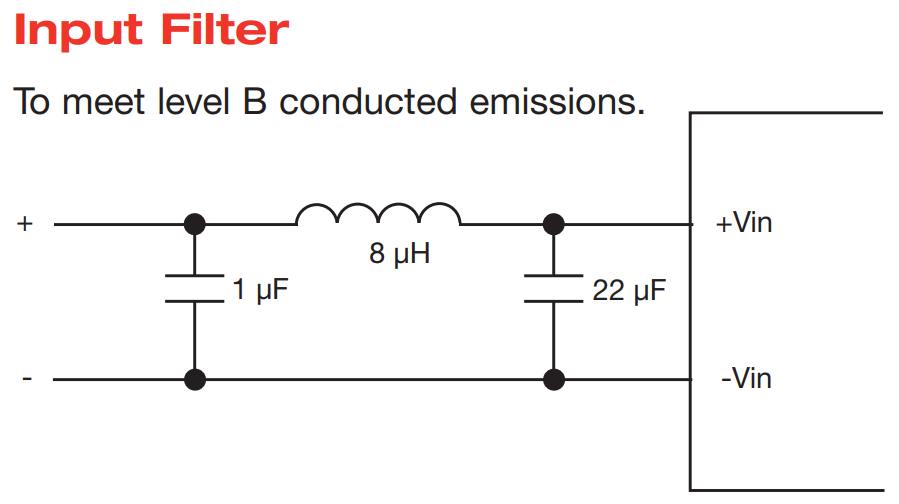
\includegraphics[scale=1.5]{content/images/emissionckt.png}
	\caption{XP Power JCA0605S05 Level B Emission Circuit \cite{isolatedvoltageconverter}}
	\label{fig:emissionckt}
\end{figure}

Applying the mentioned solutions, problems faced due to power have been dealt with and the constructed system safety is ensured.

\subsection{Mechanical Design}
In A4MCAR, the RC-Car chassis kit Tamiya TT01-E \cite{tt01e} have been used. The chassis kit consists of several parts and it is a kit that is used in professional RC-Car competitions. The Figure in \ref{fig:rccarparts} show the constructed Tamiya TT01-E chassis kit along with several other equipment that have been used in A4MCAR. Since the A4MCAR does not only have basic driving elements but also has many other equipments that are related to sensing, processing, and power, the space on the RC-Car would not be enough to hold the extra elements. Therefore, an extension to the existing chassis was needed. To solve this problem, an extension have been designed that is able to hold other elements used in the board with holders and screws. 
\begin{figure}[!ht]
	\centering
	\captionsetup{justification=centering}
	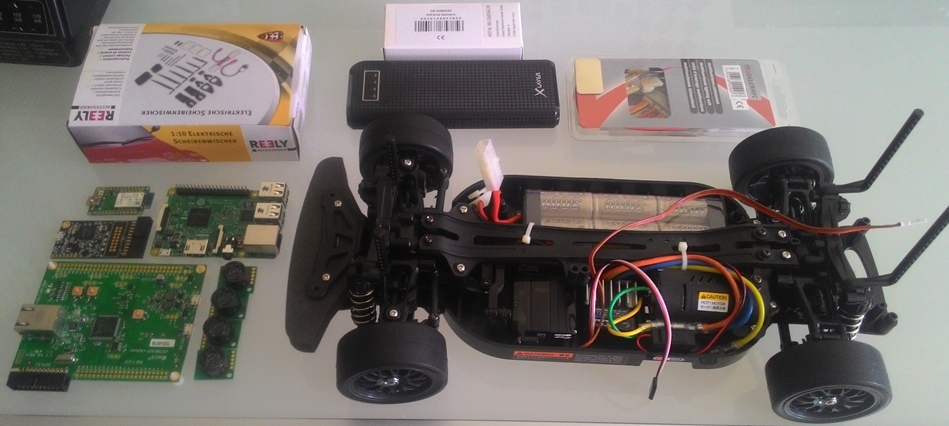
\includegraphics[width=\textwidth]{content/images/rccarparts.png}
	\caption{Tamiya TT01-E Chassis and other parts used in A4MCAR}
	\label{fig:rccarparts}
\end{figure}

An illustration of the mechanical overview that shows the designed model is shown in \ref{fig:mechanicaloverview}. This mechanical layer has been designed using a 3D model software and the software output with the .STL extension is used for the layer production using a 3D printer. Using appropriote 1mm to 2mm diameter screws, the constructed body is installed to the main chassis as an extension layer and the other elements are installed on top of this extension layer. 
\newpage
\begin{figure}[!ht]
	\centering
	\captionsetup{justification=centering}
	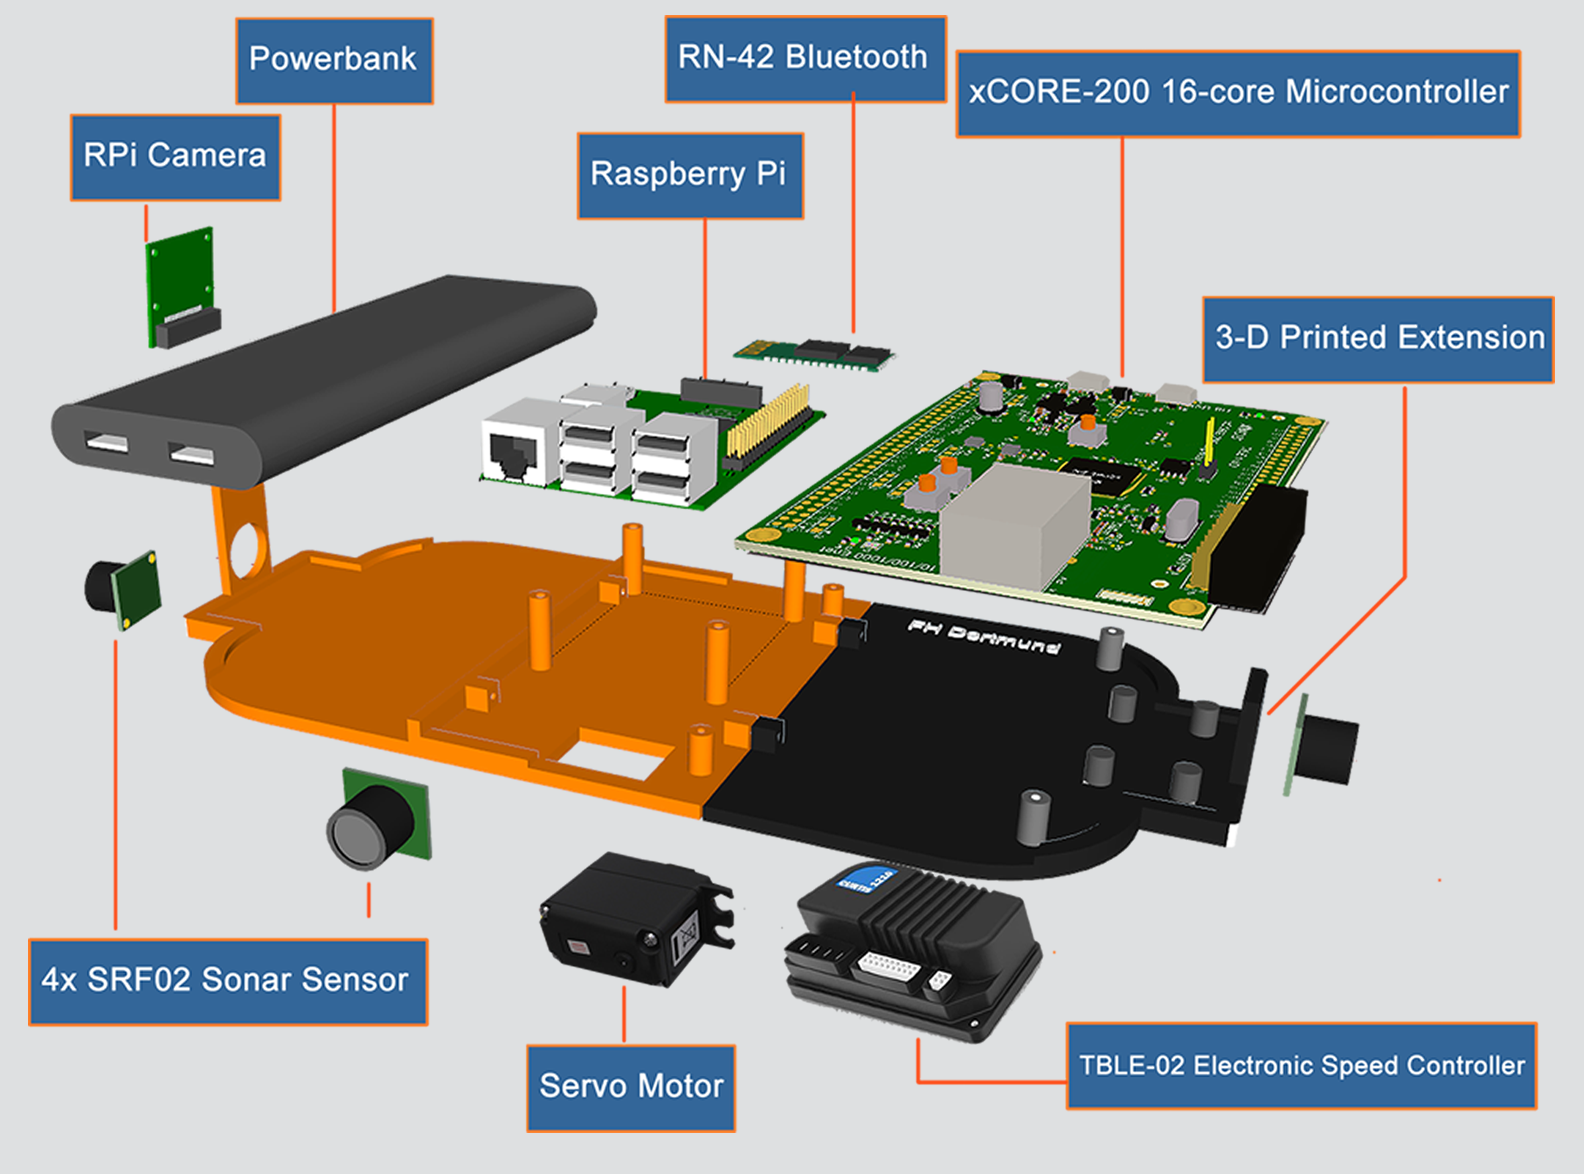
\includegraphics[scale=0.25]{content/images/mechanicaloverview.png}
	\caption{Mechanical overview of the A4MCAR}
	\label{fig:mechanicaloverview}
\end{figure}

\section{Low-Level Module Design and Implementation}
\subsection{Overview}
As mentioned in the "Low-level Module Infrastructure" subsection, Low-level module software has been implemented on xCORE-200 eXplorerKIT using the development platform xTIMEcomposer 14.2.3. While developing with xC on xTIMEcomposer, task communication is handled by channels and interfaces. In A4MCAR, for the sake of structured development with defined variable types, interfaces are more commonly used for user-defined tasks. An software design analogy of equating provided interfaces to client interfaces in xC could be made. Similarly, required interfaces could be thought of server interfaces in xC. Using this analogy, the designed software components could be illustrated with a SysML \cite{sysml} diagram as shown in Figure \ref{fig:sysmlxmostasksbrief}.
\begin{figure}[!ht]
	\centering
	\captionsetup{justification=centering}
	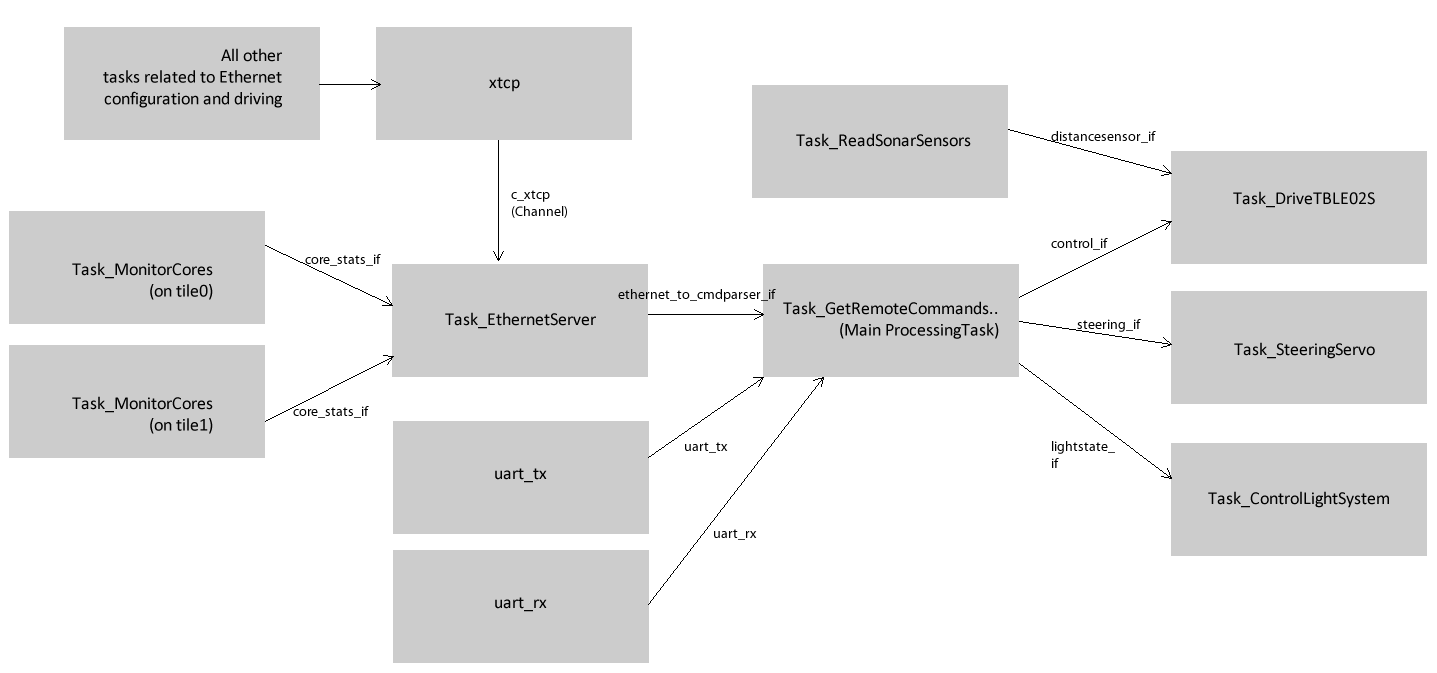
\includegraphics[width=\textwidth]{content/images/sysmlxmostasksbrief.png}
	\caption{Brief block diagram for the developed tasks and interfaces for low-level module}
	\label{fig:sysmlxmostasksbrief}
\end{figure}

The complete component diagram of the software that is developed is shown in Figure \ref{fig:sysmlxmostasks}.

\begin{figure}[!ht]
	\centering
	\captionsetup{justification=centering}
	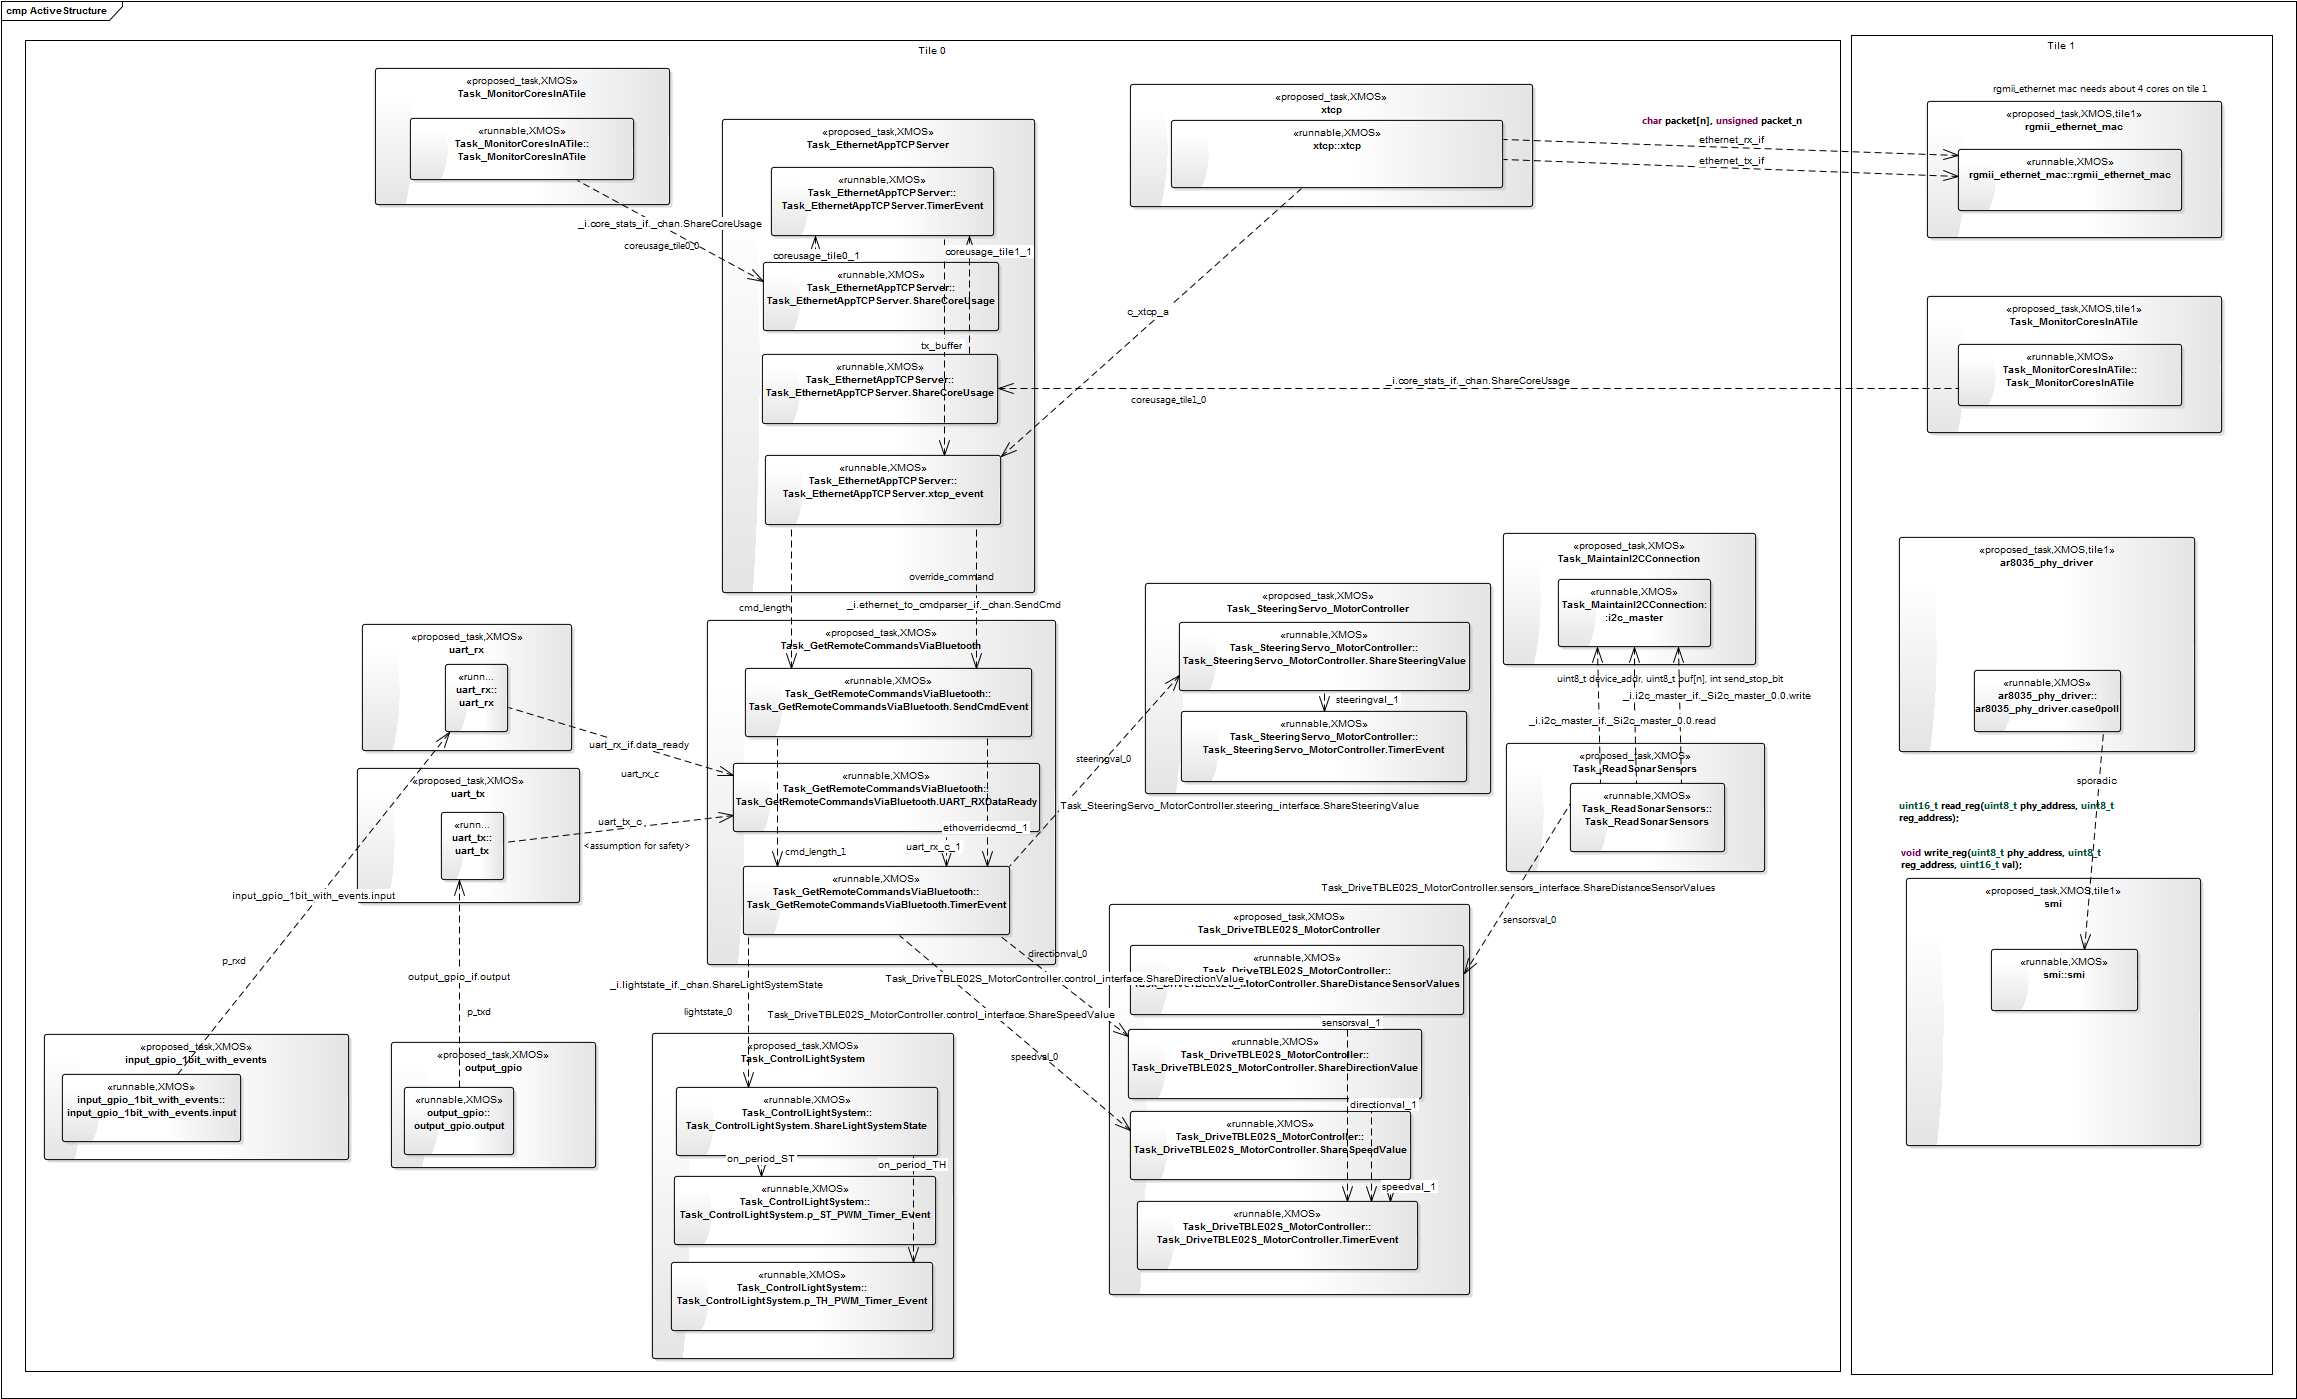
\includegraphics[scale=0.21]{content/images/sysmlxmostasks.png}
	\caption{Block diagram for the developed tasks and interfaces for low-level module}
	\label{fig:sysmlxmostasks}
\end{figure}
\newpage
In xC, two essential concepts are worthy to explain in order to understand multi tasked development. First is how a task is created and the second is how tasks are connected. A task in xC is nothing but a function that has client and server ports with interfaces. Once all functions are connected using globally instantiated interface variables they start acting as tasks. An example of how a task function is declared and how functions are placed on cores and interconnected which is also some of what is implemented for A4MCAR are shown in Listing \ref{lst_exampletaskxc} and Listing \ref{lst_howtasksconnectxc}, respectively.

\lstinputlisting[caption=An Example Task Decleration in xC, label=lst_exampletaskxc, style=xc]{content/listings/lst_exampletaskxc.txt}

In the code given with the Listing \ref{lst_exampletaskxc}, it is seen that the function prototype has several arguments as client and server interfaces. Those interfaces indicate the role of the data communication using the respective interface. When a task function takes client interface as an argument, it means that the task function sends data to that interface, whereas when a task function receives a message using event handles it is given by the server keyword.

\lstinputlisting[caption=An Example of How Tasks are Placed and Interconnected in xC, label=lst_howtasksconnectxc, style=xc]{content/listings/lst_howtasksconnectxc.txt}

The Listing in \ref{lst_howtasksconnectxc} shows in which tile and at which core a task will be places. Using the par keyword (given in Line 1), every line of code in that particular code block will be paralellized using the scheduler of xCORE. 

All the source and header files that contain task functions and that are developed in this fashion are shown in Figure \ref{fig:fullfiletree}.
\begin{figure}[!ht]
	\centering
	\captionsetup{justification=centering}
	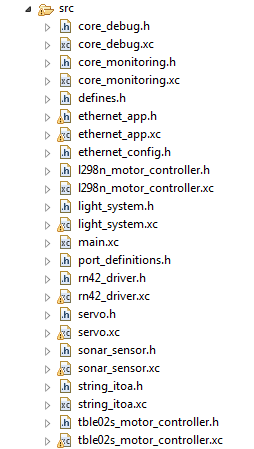
\includegraphics[scale=0.8]{content/images/fullfiletree.png}
	\caption{Full file tree for all the tasks developed for low-level module}
	\label{fig:fullfiletree}
\end{figure}
\newpage
\subsection{Actuation}
\subsubsection{Acceleration}
For acceleration and deceleration, a brushless DC motor is controlled by delivering PWM signals to the TBLE02-S Electronic Speed Controller. The task and how it is connected to other tasks can be seen in Figure \ref{fig:sysmlxmostasksbrief}. In order to deliver the desired PWM signal, a task that use timers have been created which is given in Listing \ref{lst_tble02task}. The created template of the task in Listing \ref{lst_tble02task} is not only used for the acceleration task, but also used for the other tasks that use PWM signaling to control other devices. In the task, it is seen that in order to generate the desired duty cycle, the amount of time for which the output signal must be on and off are calculated (Lines 19 through 38) and the output port is toggled (Lines 39 through 48) accordingly. The port toggling is done inside a timer event (shown in Line 17) that is dynamically delayed given the calculated on and off times.
\newpage
\lstinputlisting[caption=Created PWM signaling template, label=lst_tble02task, style=xc]{content/listings/lst_tble02task.txt}
The desired PWM pulse widths are taken from the TBLE02-S Electronic Speed Controller manual and the overall PWM period has been set to 20ms which is the standard period for most of the controllers. Since the motor speed is very high and it is not desired in our application, the pulse widths are manipulated in order to reach lower speeds in full force. The interface 'control\texttt{\_}if' (Line 9 and Line 13) is used that delivers a number between 0-100 in order to express speeding information while also delivering a direction value which is either FORWARD (0) or REVERSE (1). With this information, the developed task is able to control the acceleration of the A4MCAR. Additionaly, the acceleration task is modified in order to control acceleration using proximity sensor inputs for safety. Minimum safest front distance is set to 50 centimeters.

Acceleration task and how it data is transferred between other tasks can be seen in the software component diagram in Figure \ref{fig:sysmlxmostasksbrief} with acceleration task having the function name 'Task\texttt{\_}DriveTBLE02E'.

\subsubsection{Steering}
Steering of the A4MCAR is done with the help of a Servo motor that is also controlled with PWM signaling. As mentioned in the Acceleration subsection, the tasks that are related to PWM use the template from Listing \ref{lst_tble02task}. For steering the interface 'steering\texttt{\_}if' is used which is set to 0 for very left and 100 for very right positions. Additionally, the two changes that are made to the acceleration task (from Listing \ref{lst_tble02task}) could be listed as follows:
\begin{itemize}
	\item The pulse widths are altered in order to conform a servo motor's behavior which is usually 1.5ms pulse for stationary position, 1-1.5ms for left steering and 1.5-2.0ms for right steering. For A4MCAR, these values are set to 1.3-1.5ms for left steering and 1.5-1.75ms for right steering in order to get rid of the issue of servo motor turning more than its holding platform could handle and damaging its gears.
	\item On and off periods are calculated differently as compared to what is shown in the Listing \ref{lst_tble02task}. The Listing in \ref{lst_servotask} shows the calculation of the periods using the pulse width values.
	\lstinputlisting[caption=Calculation of on and off times for servo control, label=lst_servotask, style=xc]{content/listings/lst_servotask.txt}
\end{itemize}

Steering task and how it data is transferred between other tasks can be seen in the software component diagram in Figure \ref{fig:sysmlxmostasksbrief} with steering task having the function name 'Task\texttt{\_}SteeringServo'.

\subsubsection{Braking}
Since the motor that is used in A4MCAR is a brushed motor, it does not come with braking features. Therefore, a braking mechanism was needed to be implemented. For this purpose, a 2-channel relay board from Sainsmart (shown in Figure \ref{fig:relayboard}) has been used to short circuit the terminals of the motor when braking is required. In the Figure \ref{fig:brake}, the circuit portion that is controlling the operation of the brake is given.
%brushless motor needed, three connections (Orange connection), and mode setup. (source: tble02s manual)
\begin{figure}[!ht]
	\centering
	\captionsetup{justification=centering}
	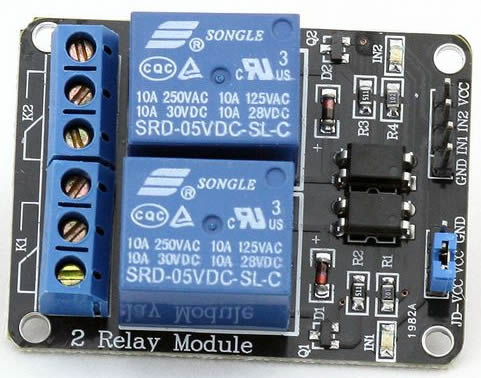
\includegraphics[scale=0.4]{content/images/relayboard.jpg}
	\caption{Two-channel relay board that is used for braking}
	\label{fig:relayboard}
\end{figure}

\begin{figure}[!ht]
	\centering
	\captionsetup{justification=centering}
	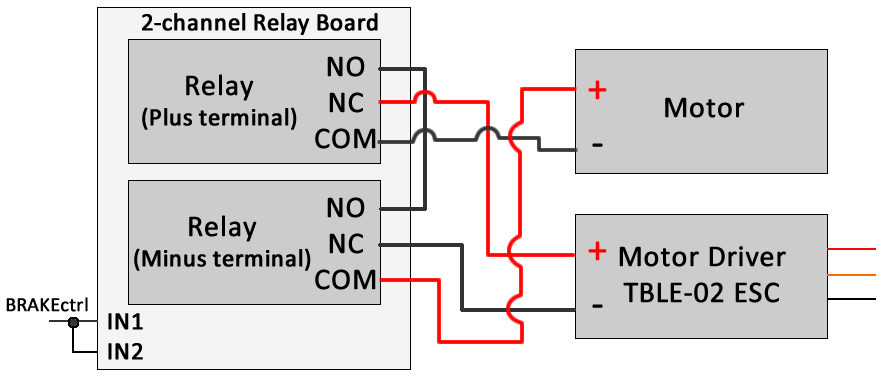
\includegraphics[scale=0.5]{content/images/brake.png}
	\caption{Relay circuit to control braking}
	\label{fig:brake}
\end{figure}

Normally, the terminals of the motor and the motor driver (Electronic Speed Controller TBLE-02) are connected together. Using the switching mechanism that is provided by the relays, motor terminals are short circuited when the relays are activated. 

Relays have three essential input or output signals that are used in operation. Those signals involve IN, NO, NC, and COM. With simple switching in mind, the operation of the relay can be described. When IN signal is low, COM is short circuited with NO whereas when IN signal is high, COM signal is short circuited to NC signal. 

By using this mechanism and using the COM signal output, motor is supplied by motor driver normally and motor terminals are short circuited when the braking is required. The control has been done by giving the same input to IN1 and IN2 signals, IN signals for each relay, from the xCORE-200 eXplorerKIT. The integration of the braking mechanism to the system is done at the acceleration task, in which when the received speed is zero, brake is activated. Since the relay works with only 5V input signal for the IN terminal, BRAKEctrl signal, given in Figure \ref{fig:brake} is connected to the xCORE-200 eXplorerKIT through a 5V to 3.3V converter, which is also shown in the schematics given in the Figure \ref{fig:RCCAR_Schematics}.

\subsection{Proximity Sensing}
As stated in the overview section, the proximity sensing is handled via four SRF-02 ultrasonic sensors connected to an I\textsuperscript{2}C network. In the software, 'lib\texttt{\_}i2c' from XMOS is used in order to handle communication with the peripheral. 

The pseudo version of the proximity sensing task is given in Listing \ref{lst_proximitysensing}. The proximity sensing task is a periodic task that polls individual ultrasonic sensors using their respective addresses (Line 12 and Line 13) in order to obtain what is the distance perceived by front, rear, left, and right sensors. In order to handle this in a modular manner, device addresses are placed in the header file. Furthermore, the task that maintains I\textsuperscript{2}C communication alongside proximity sensing task is seperated and the two tasks are connected using 'i2c\texttt{\_}master\texttt{\_}if' interface (shown in Line 1). The sensing is achieved every 0.2 seconds within a timer event (shown in Line 7) and when the sensing of each sensor complete, the value is sent by its respective interface 'distancesensor\texttt{\_}if' to the acceleration task (Line 22). 

\lstinputlisting[caption=Proximity sensing task, label=lst_proximitysensing, style=xc]{content/listings/lst_proximitysensing.txt}

Proximity sensing task and how it data is transferred between other tasks can be seen in the software component diagram in Figure \ref{fig:sysmlxmostasksbrief} with proximity sensing task having the function name 'Task\texttt{\_}ReadSonarSensors'.

\subsection{Lighting System}
The light system of the A4MCAR is a light module from the RC-Car parts producer Modelcraft that is driven with PWM. The module uses two PWM channels: one for light adjustment due to steering input, one for light adjustment due to acceleration input. Similarly to all the other PWM control tasks, PWM signal generator template that is given in \ref{lst_tble02task} has been used in order to generate correct pulse widths for the light system. The task that is given in \ref{lst_tble02task} has been adjusted to have two timer events for each PWM channel as opposed to one timer event. Desired pulse widths for several modes are contained in the header file of the light system task and these modes have been selected given the steering, angle, and gear inputs from the Bluetooth communication task. The functions regarding pulse width time generation for different light system modes have also been created. 

Light system task and how it data is transferred between other tasks can be seen in the software component diagram in Figure \ref{fig:sysmlxmostasksbrief} with light system task having the function name 'Task\texttt{\_}ControlLightSystem'.

\subsection{Bluetooth Communication}
In order to configure RN42 Bluetooth module \cite{rn42datasheet} as slave to communicate with the Android phone and receive data, UART communication have been implemented using 'lib\texttt{\_}uart' from XMOS. In order for the UART communication to be handled correctly, CTS and RTS pins of the RN42 module should be short circuited since a data flow protocol such as RS232 is not being used in our application. UART library has been configured to have a buffer size of 512 bytes and baudrate of 115200bps which is a high speed UART data rate standard that conforms many microcontrollers. Several tasks have been implemented such as uart\texttt{\_}rx, uart\texttt{\_}tx, and the Bluetooth communication task in order to implement bluetooth control feature into the A4MCAR. While uart\texttt{\_}rx and uart\texttt{\_}tx tasks handle port access and data transfer in respective directions using sporadic events, the Bluetooth communication task is responsible for configuring the Bluetooth module and receiving driving commands. For an easy communication, a string with a number of bytes is constructed and interpreted by the Bluetooth communication task. This string which we refer to as 'driving command' is given and explained in the Figure \ref{fig:bluetoothcommand}. 
\begin{figure}[!ht]
	\centering
	\captionsetup{justification=centering}
	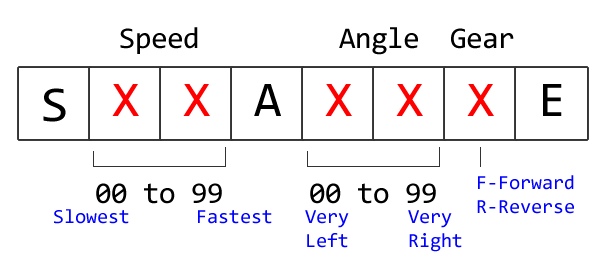
\includegraphics[scale=0.6]{content/images/bluetoothcommand.png}
	\caption{Driving command format generated to contain speed, angle, and gear information}
	\label{fig:bluetoothcommand}
\end{figure}
The command parsing and how the received data is accumulated to other tasks is given in the Listing \ref{lst_bluetoothtask}. 

The operation of this portion of the task could be explained as follows:
\begin{itemize}
	\item A preprocessor macro has been defined which is RN42\texttt{\_}INITIAL\texttt{\_}CONFIG. This macro activates the configuration function which configures RN42 module with slave mode. This configuration is shown in the Line 2 of the Listing \ref{lst_bluetoothtask}. It should be noted that the configuration should only be done once per bluetooth module.
	\item Receiving driving command using uart receive event (Line 7), integrity check for the command (Line 20), and parsing in order to obtain speed, angle, and gear values (Line 21) has been implemented.
	\item Since driving command is not the only source of actuation data source for A4MCAR and it could have overriding commands over Ethernet from high-level module image processing task, ethernet override is handled with an integrated event in the Bluetooth communication task (shown in Line 11).
	\item Reverse driving mode is not entered by the TBLE02-S Electronic Speed Controller unless the motor fully stops. To achieve this, normally user has to select reverse mode several times from the controller. In order to get rid of this issue, once the reverse command is received, software enters reverse mode a few times with very short delays, thus users can select it only once and enjoy driving without having to select the mode a few times by themselves. This implementation is shown in Line 23 in the Listing \ref{lst_bluetoothtask}.
	\item The obtained control and steering values are sent to the associated task functions in order to handle the actuation (Lines 27 through 29).
\end{itemize}
\lstinputlisting[caption=Bluetooth communication task pseudocode, label=lst_bluetoothtask, style=xc]{content/listings/lst_bluetoothtask.txt}

Bluetooth communication task and how it data is transferred between other tasks can be seen in the software component diagram in Figure \ref{fig:sysmlxmostasksbrief} with bluetooth communication task having the function name 'Task\texttt{\_}GetRemoteCommands'.

\subsection{Ethernet (TCP) Server Implementation}
TCP server of the A4MCAR low-level module acts as the only source of communication that is implemented between low-level module and high-level module. The TCP communication that is implemented for this basic data transmission and reception could be called as Telnet \cite{telnet}. As mentioned, while overriding driving command (Figure \ref{fig:bluetoothcommand}) is sent from high-level module (configured as the Telnet server) to low-level module (configured as the Telnet client), for the visualization purposes the core utilization information is sent from low-level module to high-level module. On the low-level side, library that is provided from XMOS 'lib\texttt{\_}xtcp' is used with the following adjustments:
\begin{itemize}
	\item The application notes from XMOS involves only UDP applications. This application has been manipulated in order to have TCP protocol based Telnet server
	\item The TCP server has been configured with a static IP address and with a bind port.
	\item Data receiving and transmitting event handlers as well as the interface that sends the driving command to the Bluetooth communication task have been created.
	\item Since the media-independent interface (MII) of xCORE-200 eXplorerKIT supports up to 1000Mbps reduced gigabit media-independent interface (RGMII), the ethernet server task takes up to 3 to 4 cores in order to be parallelized. In order to reduce the excessive core usage, this interface have been reduced to a speed of 100Mbps by the software that takes about 2 cores in order to be parallelized efficiently. Furthermore, it is important to mention that since application in the A4MCAR does not require a gigabit ethernet connection, this decrease in the speed did not affect the performance of the communication.
\end{itemize}

TCP server task and how it data is transferred between other tasks can be seen in the software component diagram in Figure \ref{fig:sysmlxmostasksbrief} with TCP server task having the function name 'Task\texttt{\_}EthernetServer'.

\subsection{Core and Tile Monitoring}
Core monitoring task that is responsible for finding core utilization percentage and sending it to the TCP server task is created for the two individual tiles of the xCORE-200 eXplorerKIT. By checking the status register 'XS1\texttt{\_}PSWITCH\texttt{\_}T0\texttt{\_}SR\texttt{\_}NUM' that is mentioned in the XMOS datasheet \cite{xmosdatasheet}, and polling this register with a maximum polling rate of 1250Hz, whether a core is busy or idle at a given time is detected. A code snippet that is responsible for this operation is given in Listing \ref{lst_coremonitoring}. 

\lstinputlisting[caption=Finding busy and idle cycles in XS1 architecture, label=lst_coremonitoring, style=xc]{content/listings/lst_coremonitoring.txt}

In the given listing, the status register 'XS1\texttt{\_}PSWITCH\texttt{\_}T0\texttt{\_}SR\texttt{\_}NUM' and the processor state has been read (Line 5 and Line 9, respectively) for every core in order to find which core is idle and which core is busy at that moment. 

The obtained busy and idle cycles are then converted to a percentage value with the following Equation:
\begin{equation}
core\texttt{\_}usage\texttt{\_}percentage=\frac{busy\texttt{\_}cycles}{busy\texttt{\_}cycles + idle\texttt{\_}cycles} 100
\end{equation}
Further features introduced in core monitoring task could be listed as follows:
\begin{itemize}
	\item An interface is created, that is 'core\texttt{\_}stats\texttt{\_}if' in Figure \ref{fig:sysmlxmostasksbrief}, in order to send core utilization percentage to the TCP server task. 
	\item A preprocessor macro FLOATING\texttt{\_}POINT\texttt{\_}SHOW is also created in order to find core utilization percentage in floating point format for better precision if desired.
\end{itemize}

Observing the results have showed that the user created applications for the low-level module in A4MCAR are not very time intensive and that is why some of the tasks resulted in a core utilization value that is lower than 0 percent.

Core monitoring tasks and how their data is transferred between other tasks can be seen in the software component diagram in Figure \ref{fig:sysmlxmostasksbrief} with tasks having the function names 'Task\texttt{\_}MonitorCores'.

\section{High-Level Module Design and Implementation}
\subsection{Overview}
High-level module of the A4MCAR is composed of several processes running under Raspbian \cite{raspbiandownload} distribution of Linux Operating System that is designed for Raspberry Pi 3. In the section "High-level Infrastructure", the operation of Linux kernel is briefly introduced. During the compilation, debugging and execution of the developed processes, several development platforms such as Python 2.7 shell \cite{python27}, GNU C Compiler (GCC) \cite{gcc} have been used. Although it should be noted that remote development using Eclipse IDE \cite{remotedebuggingeclipse} is also possible, the development of A4MCAR has been done using the aforementioned development platforms by connecting into the Raspberry Pi 3 using SSH connection. While the main processes involve C, C++, Python, and Bash \cite{bash} languages, via the capability of the integrated web server to serve web pages, several other scripting and markup languages such as HTML, CSS, JavaScript (with AJAX \cite{howajaxworks} and jQuery \cite{jquery} frameworks) have also been used. The operation of the user developed processes along with third party utility processes that are integrated into the system are given in the Figure \ref{fig:rpicomponents}. 
\begin{figure}[!ht]
	\centering
	\captionsetup{justification=centering}
	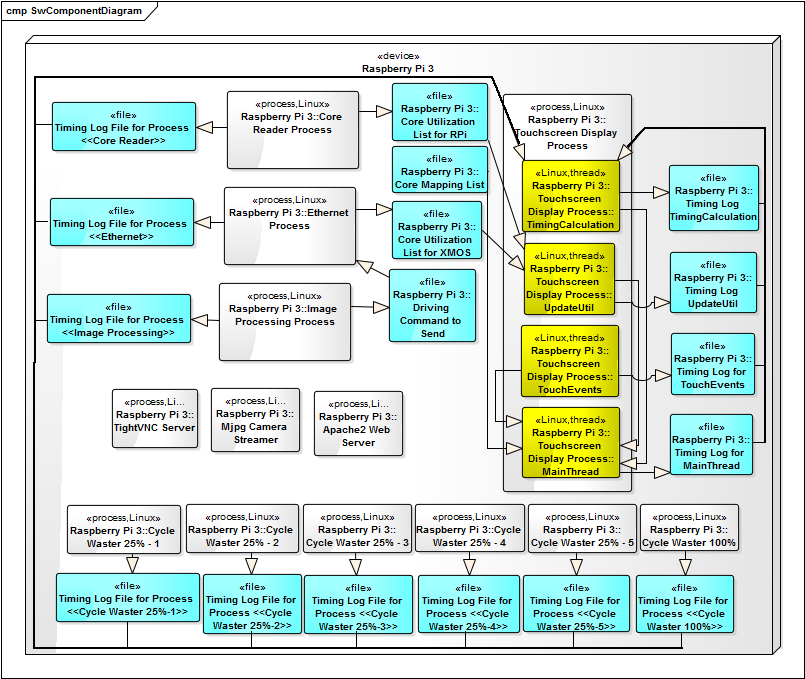
\includegraphics[width=\textwidth]{content/images/rpicomponents.png}
	\caption{High-level module software component diagram including files and file accesses}
	\label{fig:rpicomponents}
\end{figure}

Since cross development platforms using languages such as C, C++ and Python have been used in A4MCAR high-level module, the multi-tasking is handled in the process layer rather than in thread or task level. That means that each process are executables of their own using different libraries and compilers. 

In the Figure \ref{fig:rpicomponents}, it is also seen that the communication between user developed processes are handled with file accesses. All file accesses are asynchronous and there is no event to wait for data or require data within some time as it is low-level module inter-process communication. This should indicate that the communication using read-write accesses does not constrain the processes as it is in a regular inter-process communication. Furthermore, it should be noticed from the Figure in \ref{fig:rpicomponents} that although a process is able to read from many files, there is no example of two or more processes trying to write to the same file. Reading from many files is not critical, while the latter (i.e. two or more processes trying to write to the same file) should be handled by cross-process mutexes or semaphores that would be able to lock and unlock the same physical memory space from cross-processes. Although not valid in our case, it should be known that by using the existing cross-process mutexes or creating a semaphore mechanism, one should be able to allow two or more processes to write to the same file \cite{linuxkernelbook}.

The way multi-tasking is handled with this constructed software architecture (in the Figure \ref{fig:rpicomponents}) is that every process is run by an external script at the boot time (or via touchscreen interface, which is the main control interface in our case) and their scheduling is handled by the Linux kernel. While the scheduling is not manipulated, the mapping or pinning of processes to different cores and evaluating them are the focus of A4MCAR in order to find the most optimal parallelization solution.

Regarding hardware, the high-level module is connected to two devices. The interfacing of these devices, a Raspberry Pi camera v2.0 and a Touchscreen display is illustrated in the Figure \ref{fig:hwoverview}. It is seen in the figure that interfaces such as HDMI, SPI, and CSI have been utilized. In the respective sections, hardware communication and the related software will be further explained.
%%Full names as appendix  ??? MAYBE LATER
\subsection{Implemented Online Timing Features}
In order to seek an assessment technique to compare timing performance of different distributions, online timing features are implemented in the user-developed processes of the high-level module of A4MCAR. Thus, while applications are running, a performance evaluation could be done with the help of the those features. The code skeleton is developed for both Python and C,C++ applications and the applications are integrated on top of the skeleton with timing features. Therefore, it is important to understand how each application that will be discussed in the following sections are timed.

Recall that in the Scheduling section the timing properties in a scheduled system is explained that is shown in Figure \ref{fig:scheduling}. By making use of the figure, limitations of implementations and the implemented timing features could be listed as follows:
\begin{itemize}
	\item Because the values such as IPT, CETs and RT (referred from the Figure \ref{fig:scheduling}) are out of our reach since they are hidden in the Linux kernel, in the online timing analysis features that are implemented, the aforementioned values have been neglected. With offline scheduling analysis, however, CET values could be easily obtained.
	\item Recording the the start and end times of execution using an accurate clock. For that purpose, in computers there are two types of clocks: (1)- User CPU clock and (2)- System CPU clock. While user CPU clock is used for finding out how long it has passed since the program has started, the system CPU clock takes place in the kernel space and measures how long it has passed since 1st of January, 1970. The latter clock was found as the viable solution as user CPU clock would not allow comparison along the entire Linux kernel. In the code, functions time.time() for Python and clock\texttt{\_}t clock() have been used in order to record start and end times more accurately \cite{cpuandusertimes} \cite{cpuandusertimes2}.
	\item Finding the execution time (ET) of one iteration using the following Equation, provided that start\texttt{\_}time is the time recorded before the iteration and end\texttt{\_}time is the time recorded after the iteration. The units are all seconds.
	\begin{equation}
	execution\texttt{\_}time=end\texttt{\_}time - start\texttt{\_}time
	\end{equation}
	In the version that is developed for C language, since clock\texttt{\_}t is able to measure clock cycles rather than seconds, the Equation is changed to the following:
	\begin{equation}
	execution\texttt{\_}time=\frac{end\texttt{\_}time - start\texttt{\_}time} {CLOCKS\texttt{\_}PER\texttt{\_}SEC}
	\end{equation}
	
	\item Finding the slack time (ST) is one of the most important tasks that is within the scope of the online timing features because as a rule of thumb, we could assess the timing performance by saying that if a process has a higher slack time than before, it means that that task is better utilized compared to before as the idle time the CPU is doing some other task is more than what it used to be. The slack time of a previous iteration is measured by the following Equation, provided that the calculation takes place right after start time is recorded and IPT is neglected. It should also be noted that the C language version could be created by dividing the clock cycles with the clock cycles per second (CLOCKS\texttt{\_}PER\texttt{\_}SEC) in the same manner as execution time.
	\begin{equation}
	previous\texttt{\_}slack\texttt{\_}time=start\texttt{\_}time - end\texttt{\_}time
	\end{equation}
	
	\item In order to keep a constant period while the process is being scheduled, the processes are delayed dynamically between each iteration. Thus, processes which have a constant period could be modeled easier. In order to achieve a constant period each process are delayed by the following:
	\begin{equation}
	delay\texttt{\_}time=period - execution\texttt{\_}time
	\end{equation}
	However, if the execution time of a process is bigger than its period, that process could be counted a process that missed its deadline, given that its period is equal to its deadline due to practicality. In addition, it should be known that the deadline miss percentage is another important criteria in order to assess parallelization quality as it is normally undesired to have missed deadlines. In case of a missed deadline in A4MCAR, the process is not delayed.
	
	\item As seen in \ref{fig:rpicomponents}, there are many timing log files that are created. Those timing log files are created within every user-defined process and later are used in the Touchscreen Display application.
\end{itemize}

While each processes are constructed in the manner that is explained, the overall online evaluation is handled within the Touchscreen Display process, the process that is able to show utilization results. In the "Information Tracing and System Management" section, the details about these will be given.

An example of the timing skeleton for Python-running processes are given in the Listing \ref{lst_timingskeleton}. The user-defined Python-running applications have been created using this template, and the space that is left for task content is used for the actual features of that task.

\lstinputlisting[caption=Online timing features implemented in Python language, label=lst_timingskeleton, style=python]{content/listings/lst_timingskeleton.txt}

In the given code by the Listing \ref{lst_timingskeleton}, following remarks should be made:

\begin{itemize}
	\item Lines 2 through 5 indicate which libraries are used.
	\item Between the Lines 8 and 13, global variables to hold the time values are initialized.
	\item A timing data logging function is created (Lines 15 through 33). In this function, timing log file is opened (Lines 23 through 26), execution time is calculated after end time is recorded (Line 27 and Line 28) and then all the timing values at that instant is written into the opened text file (Lines 29 through 33). After the write operation the file is closed (Line 33).
	\item In the loop section of the process start time and previous slack time are recorded (Lines 37 through 38) before the actual task content (Lines 40 through 42) is executed. After the task content is executed, timing log is created by using the timing data logging function (Line 45) and then the task is delayed according to its period by finding the delay\texttt{\_}time that was given in (4.5). This delay operation is also given in the Listing \ref{lst_timingskeleton} at the Lines 48 through 49.  
\end{itemize}

\subsection{Core Reader}
To help with the utilization assessment and visualization purposes, a core reading process is developed that monitors cores every three seconds and writes the core usage information to a text file. For that purpose, the 'psutil' module \cite{psutil} from Python is used. The 'psutil' module allows to find information of Linux processes and cores. The core usage information for four cores of Raspberry Pi that is logged into a text file is then used for visualization in the web interface and the touchscreen interface. 

With the help of a simple function the core usage information is easily retrieved. The function is given in the Listing \ref{lst_psutil}. It should be noted that 'd' in the listing is an array with 4 elements, each of which indicating core usage for individual cores.

\lstinputlisting[caption=Psutil function to retrieve core utilization information , label=lst_psutil, style=python]{content/listings/lst_psutil.txt}

\subsection{Ethernet (TCP) Client Implementation}
In the section "Low-level Module Implementation", TCP server implementation using the xCORE-200 eXplorerKIT has been discussed. In order to maintain a sound data communication between low-level module and high-level module, a TCP client process is implemented in the high-level module. Since Python language offers very stable and easy-to-use threading support and exception handling, the TCP client implementation is done using Python. The 'socket' library \cite{socketpython} in Python is capable of delivering several functions and objects that are used for this purpose. The TCP client has been configured to have non-blocking data reception with 0.5 second period and with a timeout of 2 seconds. While the data reception is handled by an additional thread, operations such as connecting to the server, binding to the server port, and sending data periodically is handled in the main thread. The overriding driving command which is send to the low-level module is read from file before data transmission. It should be also noted that after the data reception the content is written to the file which is responsible for holding low-level module core usage information. This communication between high-level module and low-level module is illustrated in the deployment diagram given by the Figure \ref{fig:ethernetdeployment}.

\begin{figure}[!ht]
	\centering
	\captionsetup{justification=centering}
	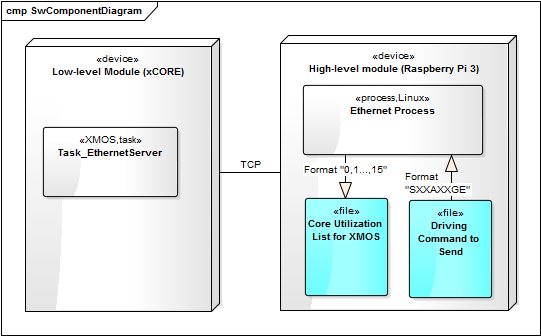
\includegraphics[scale=0.7]{content/images/ethernetdeployment.png}
	\caption{Deployment diagram showing Ethernet communication}
	\label{fig:ethernetdeployment}
\end{figure}

\subsection{Web Server and its Applications}
\subsubsection{Web Server}
In order to develop a web interface for the A4MCAR, a web server is installed and configured to the high-level module. Web servers are responsible for processing HTTP requests and delivering HTTP responses \cite{apacheguide}. The HTTP requests and responses are usually visualized using a web browser from clients in the form of web pages \cite{apacheguide}. In A4MCAR high-level module, Apache 2 web server is installed and configured as the web server since it is an open-source, robust, light-weight cross-platform that has a large user community. Additionally, another reason Apache 2 is selected is that it is capable of serving for script languages such as PHP and Python, which are used in A4MCAR applications.

Just like a Telnet server, a web server is bind to a port in a wireless or wired network. Although for different communication channels one could use different ports, web servers usually use the port number 80. Another difference of a web server is that unlike a telnet server, the data that is sent and interpreted is in the HTTP (HyperText Transfer Protocol) \cite{webserver} format unlike the TCP (Transmission Control Protocol) format. How web servers and web browsers work in order to help us visualize web pages is illustrated with the Figure \ref{fig:webserver} \cite{webserver}. \\

\begin{figure}[!ht]
	\centering
	\captionsetup{justification=centering}
	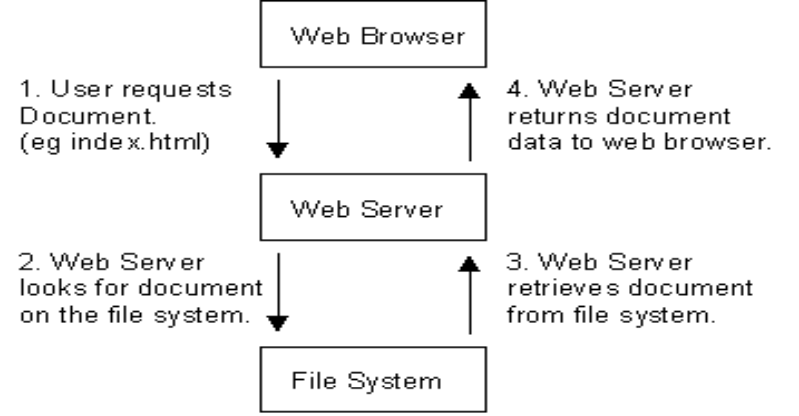
\includegraphics[scale=0.5]{content/images/webserver.png}
	\caption{How web servers and web browsers work illustrated \cite{webserver}}
	\label{fig:webserver}
\end{figure}

%ajax Eventlere bagliyor http requestleri javascript kullanarak. jQuery de isleri kolaylastirmak icin
The following technologies have been used in order to create dynamical webpage:
\begin{itemize}
	\item \textbf{HTML:} This markup language is used for defining how body elements are located in a web page and including scripts.
	\item \textbf{CSS:} CSS is used for defining the style of body elements. Borders, background properties, colors, button styles, positioning of elements are defined with CSS language.
	\item \textbf{JavaScript:} The JavaScript language is used for defining animations, as well as how events would behave.
	\item \textbf{jQuery:} jQuery \cite{jquery} is a JavaScript framework that is written using JavaScript which helps to use define scripts easier than it is with the JavaScript. It is open-source and widely used in almost every web page.
	\item \textbf{AJAX:} AJAX \cite{howajaxworks} is another framework for JavaScript which is used for handling dynamical HTTP requests without having to refresh the page. With the objects it delivers, events such as key press, mouse events, conditional events could be sent to server and processed. The returned data could be processed using JavaScript in order to dynamically update the page content \cite{howajaxworks}. This mentioned working principle is illustrated in the Figure \ref{fig:ajaxpng} \cite{howajaxworks}. 
	\begin{figure}[!ht]
		\centering
		\captionsetup{justification=centering}
		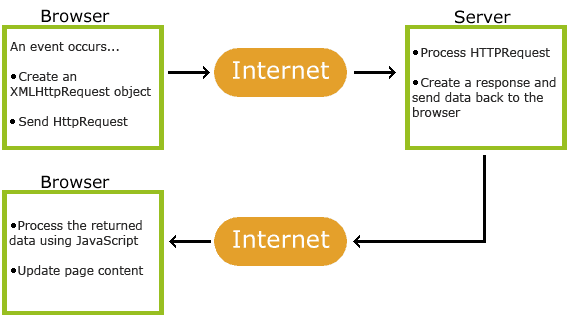
\includegraphics[scale=0.7]{content/images/ajax.png}
		\caption{How AJAX works \cite{howajaxworks}}
		\label{fig:ajaxpng}
	\end{figure}
\end{itemize}

\subsubsection{Web Page Design and Implementation} 
The web page that has been designed for users is shown in the Figure \ref{fig:web}. In the web page, it is seen that a camera stream, control buttons and sliders, and an information graph that shows core utilization in both high-level and low-level module are embedded. For the static design of the web page HTML and CSS are used, while the dynamical behavior of the web page is supported with jQuery, AJAX, and Python. The dynamical behavior of the individual parts of the web page will be explained in the following sections.
\begin{figure}[!ht]
	\centering
	\captionsetup{justification=centering}
	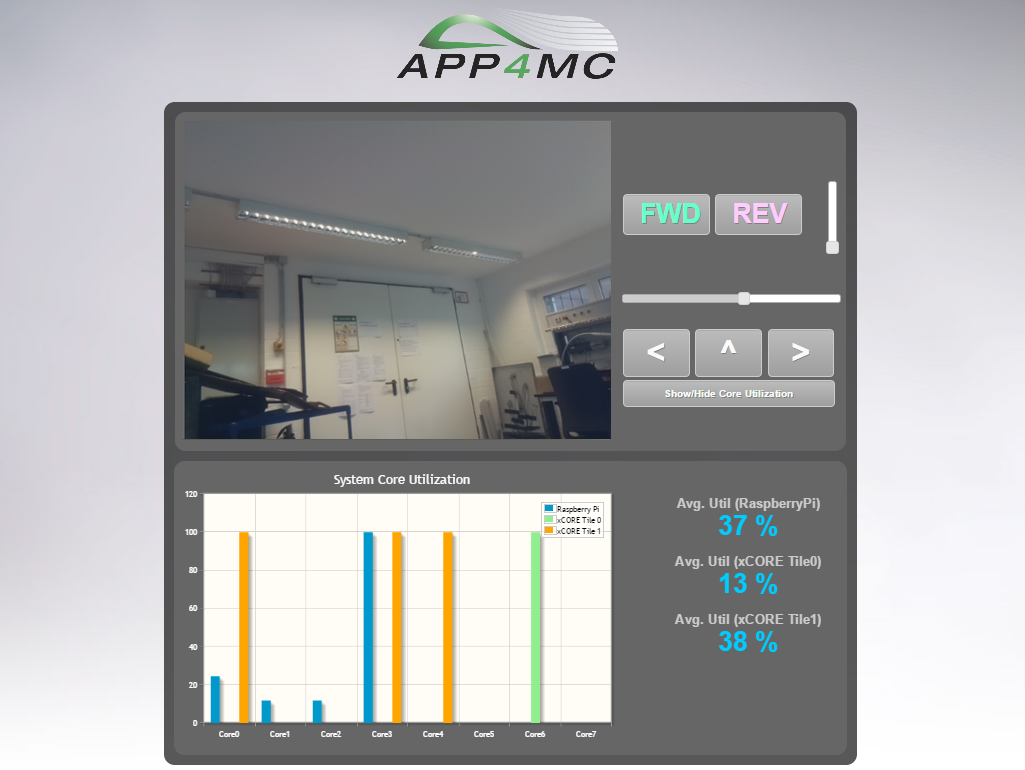
\includegraphics[width=\textwidth]{content/images/web.png}
	\caption{Web interface of A4MCAR}
	\label{fig:web}
\end{figure}

The overall dynamical behavior of the web page is illustrated in component diagram that is seen in the Figure \ref{fig:weboverallbehavior}. In the diagram, it should be noticed that the server page jqueryControl.php is the main web interface. It has some server pages and files embedded to it in order to function as a whole to deliver the features of controlling A4MCAR, core utilization display, and camera streaming. In the following subsections, each of these tasks will be explained using the component diagram shown in the Figure \ref{fig:weboverallbehavior}.

\begin{figure}[!ht]
	\centering
	\captionsetup{justification=centering}
	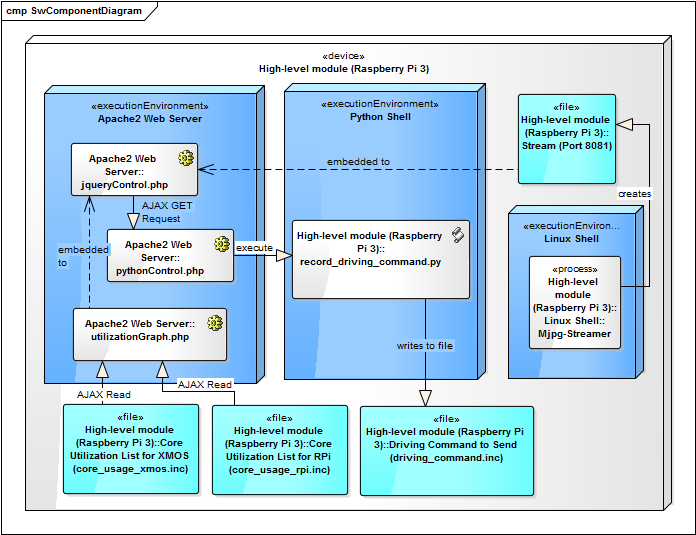
\includegraphics[width=\textwidth]{content/images/weboverallbehavior.png}
	\caption{Component diagram showing how communication inside the created web-interface works}
	\label{fig:weboverallbehavior}
\end{figure}

\subsubsection{Controlling A4MCAR via Web Page}
At the top right of the Figure \ref{fig:web}, the controls to drive the A4MCAR over web interface is shown. It is seen that there are gear selection buttons such as Forward (FWD) and Reverse (REV), along with two sliders. The sliders are created using the third party script library called 'jquery\texttt{\_}ui'. While the vertical slider is for speed adjustment, the horizontal slider is used for angle adjustment. Additionally, to select the very left, straight, and very right angles the arrow buttons could be used. 

With the help of jQuery and AJAX' ability to create event handlers within server pages, on a button press or when slider position is changed, an event handler is run that collects the position and gear information and sends it using an HTTP "GET" request dynamically to another server page called pythonControl.php (shown in Figure \ref{fig:web}). With the idea of demonstrating a basic AJAX request, an example of this is given in the Listing \ref{lst_ajax}.

\lstinputlisting[caption=Sending dynamic HTTP GET requests using jQuery , label=lst_ajax, style=jquery]{content/listings/lst_ajax.txt}

As it is seen from the Listing \ref{lst_ajax} url field, the information that is sent is nothing other than the format defined for the bluetooth communication in the low-level module, which is given in \ref{fig:bluetoothcommand}. In the Figure \ref{fig:web}, it is seen that after the information is received by pythonControl.php, using the ability of PHP to run a shell script, a Python script is run using the Python shell automatically. The python script, whenever executed, writes the received driving command information into the text file that holds the driving command. This operation is done asynchronously. How the driving command is sent afterwards is explained in the section "Ethernet (TCP) Client Implementation".
\subsubsection{Camera Streaming}
For the camera streaming, the third party module mjpg-streamer \cite{mjpgstreamergithub} has been used. This module is able to communicate over CSI interface in order to generate a stream on a network port, which then could be embedded to web pages. It is seen on the Figure \ref{fig:weboverallbehavior} how this module works along with the Apache2 Web Server. 

For the stream, Raspberry Pi camera version 2.0 with CSI interface is used which is shown in the Figure \ref{fig:rpicam20}.

\begin{figure}[!ht]
	\centering
	\captionsetup{justification=centering}
	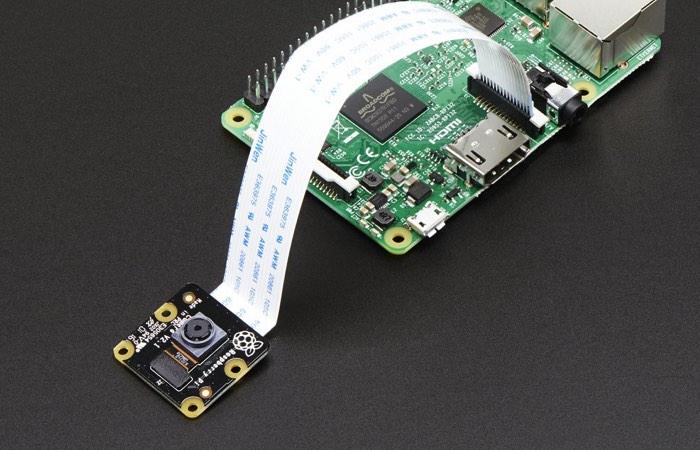
\includegraphics[scale=0.5]{content/images/rpicam20.jpg}
	\caption{Raspberry Pi camera v2.0}
	\label{fig:rpicam20}
\end{figure}

Based on the documentation of the mjpg-streamer, a script using Bash language is created which is used for generating a web stream with the correct parameters. These parameters involve resolution, frames per second, quality value, and port on which the stream will be generated. For the case of A4MCAR, the experimental version of mjpg-streamer has been used which is able to stream using the Raspberry Pi camera besides a webcam. By using the experimental version library, the following setup is found to give robust performance:
\begin{itemize}
	\item Resolution:        640x480
	\item Frames per second: 30
	\item Quality:           default
	\item Port:              8081
\end{itemize}
\subsubsection{Core Utilization Display}
Core utilization display is shown at the bottom of the Figure \ref{fig:web}. It is responsible for gathering all the core usage information from the files, displaying a graph showing percentages, and calculating average core utilizations. These operations are handled within the server page core\texttt{\_}usage\texttt{\_}read\texttt{\_}rpi.php as shown in the Figure \ref{fig:weboverallbehavior}. This server page is embedded into the main web interface which is jqueryControl.php.

For the efforts regarding creating a graph, a third party script library called 'jqPlot' \cite{jqplot} which runs within the jQuery framework is used.  The jqPlot offers various functions in order to create various plots such as bar graphs, line graphs, pie charts and 3D plots. In order to embed the plots into the web page, AJAX has been used.

\subsection{Dummy Loads}
In order to fully utilize the developed parallel software on the high-level module under full load, several processes have been created which do dummy operations to use a certain percentage of the cores. To create dummy loads, two ideas are investigated:
\begin{itemize}
	\item \textbf{Basic load with very short periods:} While using this methodology achieves certain core percentage loads, having a very short delay is considered to be non model-safe and since periods of the processes are very short, timing logs resulted in deadline misses for further analysis. Therefore, a new method of using bigger load with bigger periods is analyzed.
	
	\item \textbf{Bigger load with bigger periods:} While using a bigger load with bigger period is also viable in achieving certain core percentages, the fluctuation in the core utilization values higher than the previous option. This fluctuation is trivial in our application as most of the processes behave this way.
	
	\lstinputlisting[caption=Dummy load created with Python , label=lst_dummyload, style=python]{content/listings/lst_dummyload.txt}
	
	In order to create the dummy loads in the code, matrix multiplication of random 1000 by 1000 matrices is processed. Python offers libraries to create those matrices as well as to multiply them. The basic load that is written in Python is given with the Listing \ref{lst_dummyload}.
	
	While various loads with the same matrix operation are created, it should be noted that they differ in their iteration periods which helps to achieve different core utilization percentages. The Table \ref{tbl_dummyloads} is a list of all dummy processes that are created in order to help with the utilization research:
	
	\begin{table}[h!]
		\begin{tabular}{|l|l|l|l|}
			\hline
			Process Name & File Name & Period & Core Utilization \\
			\hline
			\hline
			CycleWaster25\texttt{\_}1 & burn\texttt{\_}cycles\texttt{\_}around25\texttt{\_}1.py & 1.4 second & 25 percent \\
			\hline
			CycleWaster25\texttt{\_}2 & burn\texttt{\_}cycles\texttt{\_}around25\texttt{\_}2.py & 1.4 second &  25 percent \\
			\hline
			CycleWaster25\texttt{\_}3 & burn\texttt{\_}cycles\texttt{\_}around25\texttt{\_}3.py & 1.4 second &  25 percent \\
			\hline
			CycleWaster25\texttt{\_}4 & burn\texttt{\_}cycles\texttt{\_}around25\texttt{\_}4.py & 1.4 second &  25 percent \\
			\hline
			CycleWaster25\texttt{\_}5 & burn\texttt{\_}cycles\texttt{\_}around25\texttt{\_}5.py & 1.4 second &  25 percent \\
			\hline
			CycleWaster100 & burn\texttt{\_}cycles\texttt{\_}around100 & 0.50 second & 100 percent \\
			\hline
		\end{tabular}
		\caption{Dummy load processes running in high-level module}
		\label{tbl_dummyloads}
	\end{table}
	
\end{itemize}

\subsection{Image Processing with OpenCV}
Some text will come here! \\
\begin{figure}[!ht]
	\centering
	\captionsetup{justification=centering}
	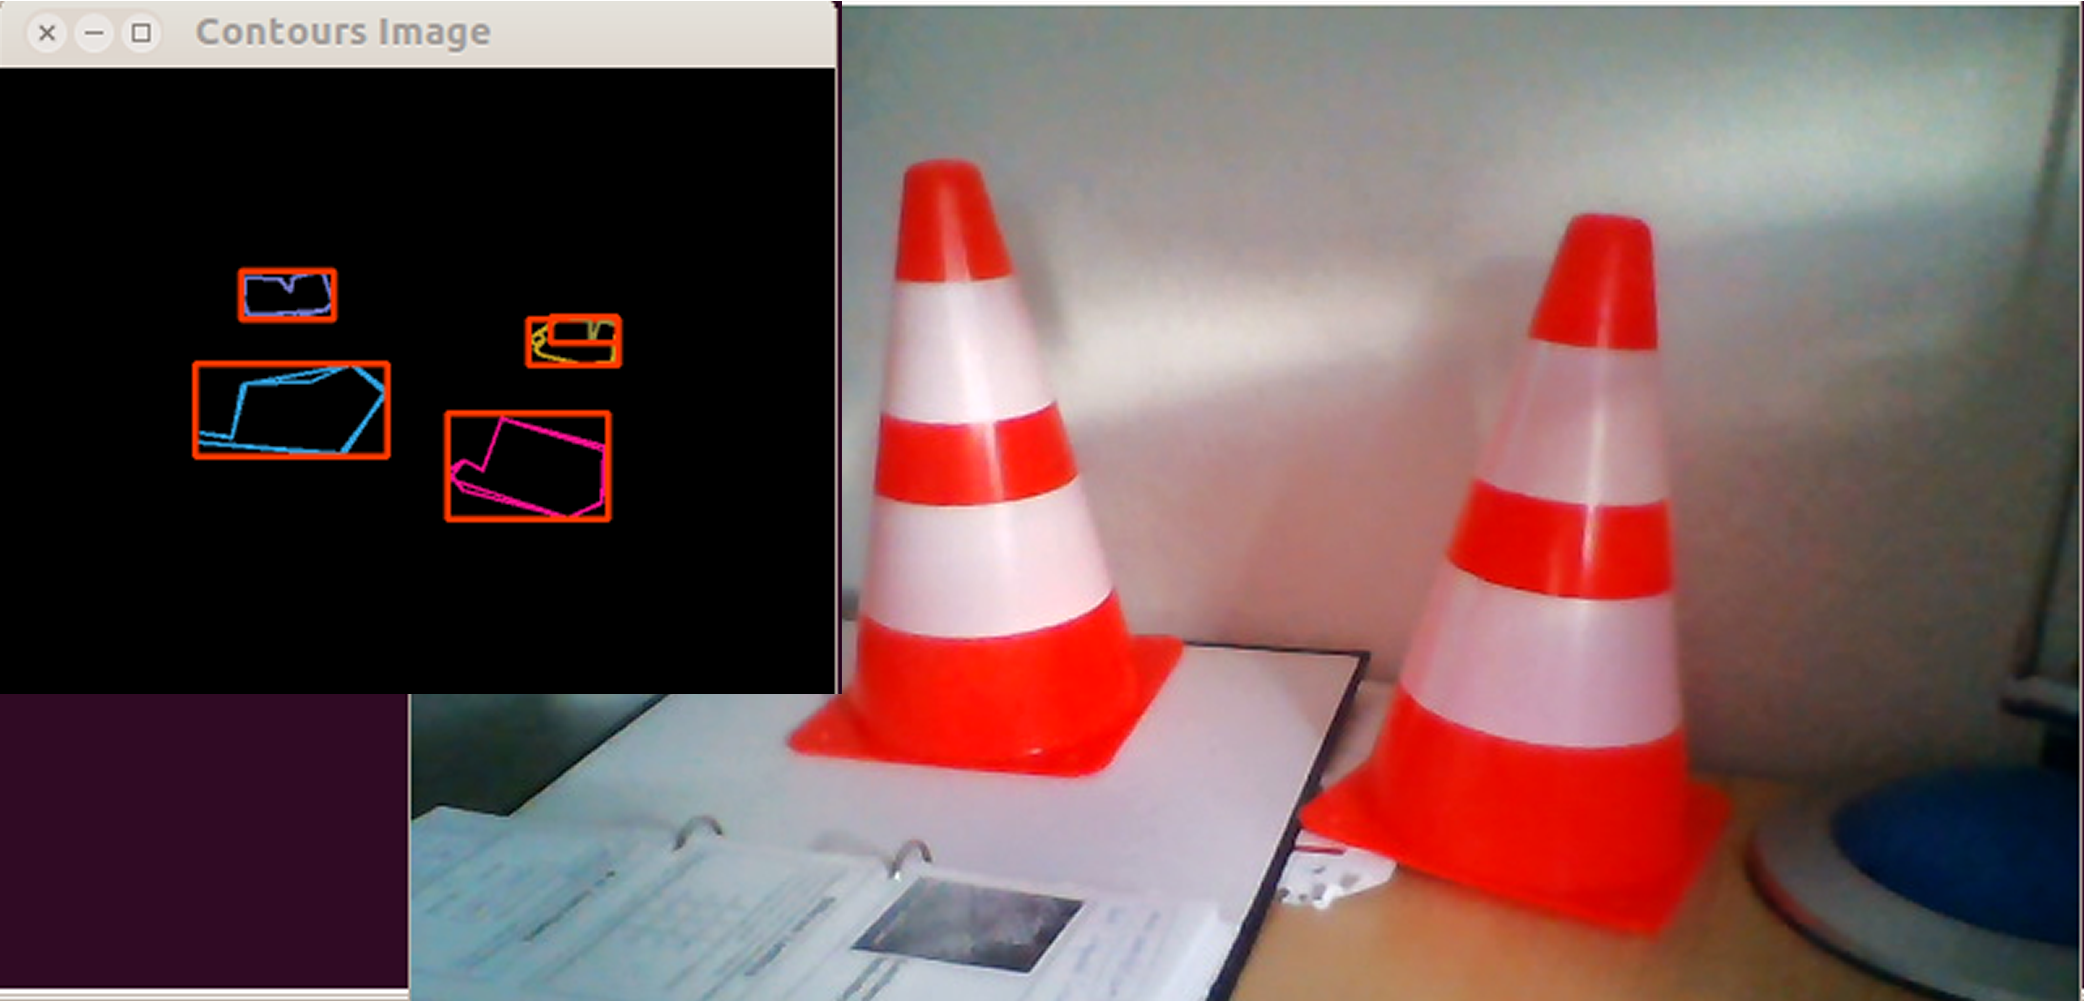
\includegraphics[scale=0.15]{content/images/traffic_cone_detection.png}
	\caption{Developed Image Processing Application}
	\label{fig:traffic_cone_detection}
\end{figure}
\subsection{Touchscreen Display}
%Add state machine diagram for display modes
\subsubsection{Touchscreen Display Features}
Touchscreen display that is embedded onto the Raspberry Pi 3 features several functions. It can not only show core utilization graph, average utilization percentages, timing performance, but also can be used to manage and allocate the processes of the high-level module. It also features connectivity settings in order to connect to an access point. Main interface and buttons are shown in the Figure \ref{fig:displaybuttons}. Using those buttons users can switch between display modes that are mentioned, as well as go to the Settings menu, exit the touchscreen application, and shutdown the Raspberry Pi. 
\begin{figure}[!ht]
	\centering
	\captionsetup{justification=centering}
	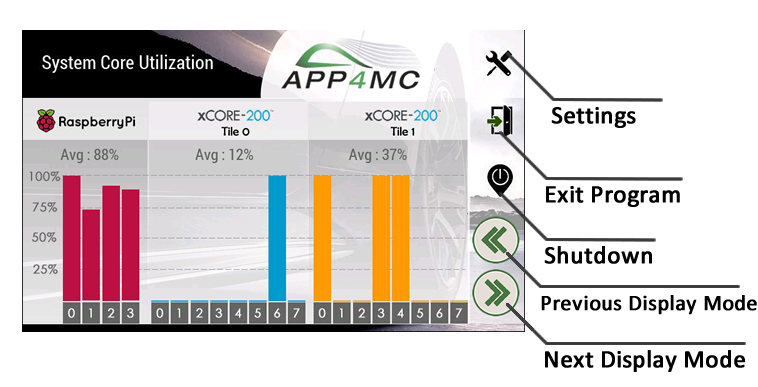
\includegraphics[scale=0.5]{content/images/displaybuttons.png}
	\caption{Button functions of A4MCAR Touchscreen Display}
	\label{fig:displaybuttons}
\end{figure}

\subsubsection{Touchscreen Display Implementation}
 %explain used libraries pygame, psutil and touchscreen interfacing hdmi etc...
%Linux tools and created .sh scripts will be in Section (5)
%Maybe add how graph is made...
As for the hardware, 5 inch HDMI touchscreen module from Waveshare has been used. This module can act as a primary monitor for Raspberry Pi. Addinitionally, the module features touchscreen controls using SPI pins of the Raspberry Pi GPIO. The module driver is installed and calibrated on Raspberry Pi in order to use the module as a primary monitor. 

The touchscreen display process uses a third-party library from Python that is called Pygame \cite{pygame}. This library is exclusively developed for creating Python language based games but it is also useful for creating graphical interfaces. After the images for the interface have been designed, the main interface has been created using the functions from Pygame. 
\begin{figure}[!ht]
	\centering
	\captionsetup{justification=centering}
	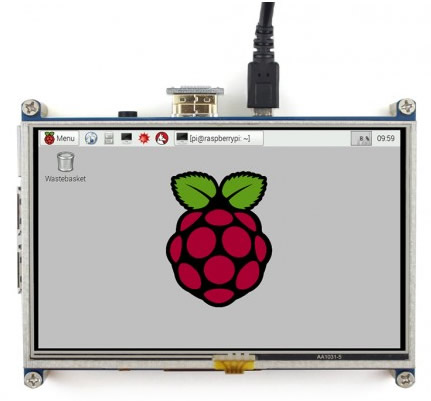
\includegraphics[scale=0.6]{content/images/touschreen5inc.jpg}
	\caption{5 inch Touchscreen module from Waveshare}
	\label{fig:touschreen5inc}
\end{figure}

Pages that are developed for the touchscreen module is shown in the Figure \ref{fig:displays}. In order to understand the behavioral operation of the touchscreen process, the Figure in \ref{fig:TouchscreenProcessSM} should be observed in parallel with the Figure \ref{fig:displays}. 
\begin{figure}[!ht]
	\centering
	\captionsetup{justification=centering}
	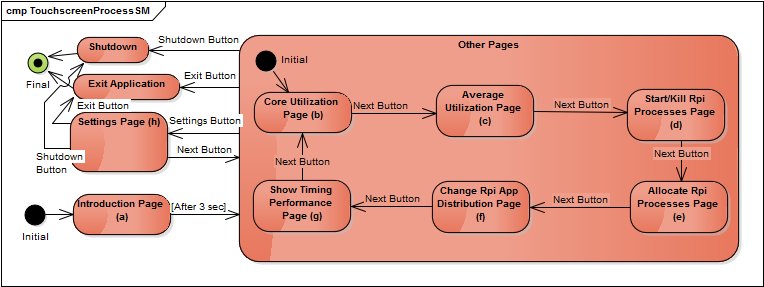
\includegraphics[width=\textwidth]{content/images/TouchscreenProcessSM.png}
	\caption{State machine of touchscreen process for pages as modes}
	\label{fig:TouchscreenProcessSM}
\end{figure}
\begin{figure}[!ht]
	\centering
	\captionsetup{justification=centering}
	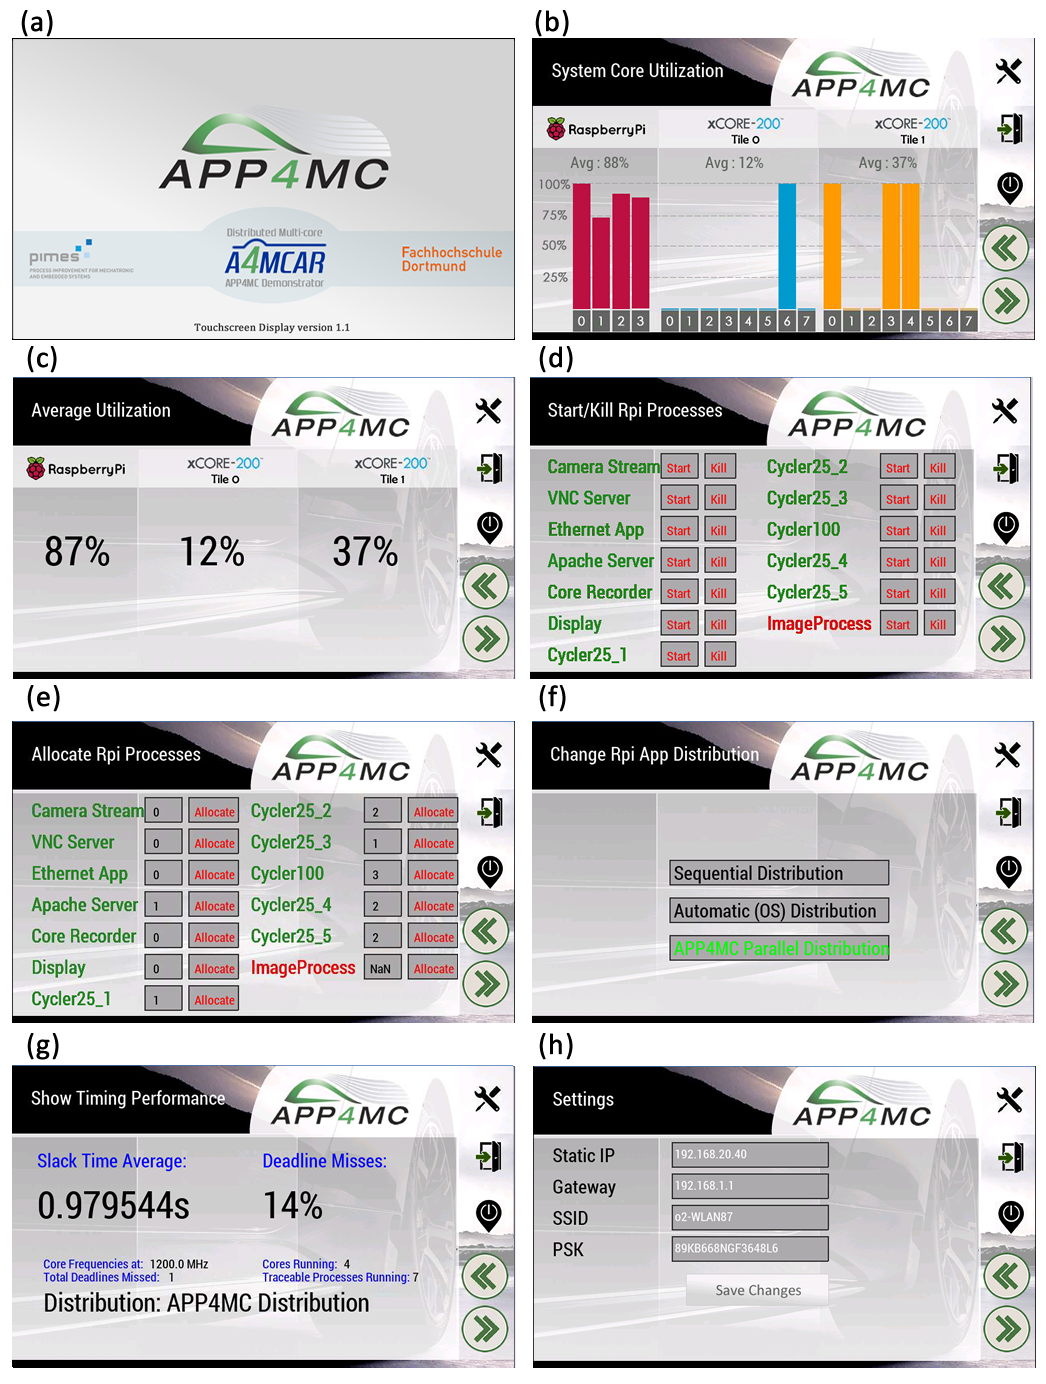
\includegraphics[width=\textwidth]{content/images/displays.png}
	\caption{Display modes from A4MCAR Touchscreen Display}
	\label{fig:displays}
\end{figure}

The introduction page that is shown in Figure \ref{fig:displays} (a) is entered as the process is started. After displaying the logo for 3 seconds, other pages are entered. The pages (b) through (g) (shown in Figure \ref{fig:TouchscreenProcessSM}) is navigated with the help of the Next button in this state. Users can browse the settings page, shutdown or exit the touchscreen display process by clicking to the respective buttons.

Since the touchscreen display process is responsible from displaying many information, libraries to gather up such information have been used. Furthermore, the data that is gathered in the timing logs and core usage logs have also been used in this application. Information that is gathered involve core usage percentages of both low-level and high-level modules, slack times of high-level processes, core frequency of high-level module, active cores count for the high-level module and core mapping list from the high-level module. The detailed information on how the information is extracted will be explained in the Section 5.

\subsection{VNC Server}
Virtual Network Computing (VNC) is a system that allows creating and managing virtual computers as well as connecting to them remotely \cite{vncmagazine}. While dealing with programming single board computers such as Raspberry Pi, it is used for viewing the single board computer desktop remotely. During the development of A4MCAR, a third-party application called XtightVNC is installed to both the Raspberry Pi and the development computer in order to connect to it without having to use external hardware.  The VNC server that is installed in Raspberry Pi, XtightVNC, is run at boot time and scheduled like any other process on the Raspberry Pi. While the server has not been manipulated during the development, in order to investigate the parallelism efficiency, this third party application should also be considered in order to get more accurate results. Further information regarding parallelism findings will be given in Section 5 and Section 6. 

\section{Android Application Implementation}
To control the A4MCAR remotely via communicating with the RN42 bluetooth module that is connected to the low-level module, A4MCAR control application is developed using Android \cite{androidwebsite} environment. In the Figure \ref{fig:tasksoverall}, one can see how developed A4MCAR control application interacts with the entire software that is developed for A4MCAR. 

As an integrated Android development environment, Android Studio \cite{androidstudio} is used. Using Android Studio, developers can not only design XML-based user interfaces for their applications, but also can describe the behavior of their programs using Java programming language. Additionally, Android Studio can emulate many of the available Android devices to help the developers debug their software. 

The developed Android application interface is given in Figure \ref{fig:androidapp}. In the figure, it is seen that the interface consists of a joystick and gear buttons that helps in constructing the driving command that was given by the Figure in \ref{fig:bluetoothcommand}. Furthermore, using a bluetooth device list, A4MCAR could be paired with and then connected in order to start data communication.

For the joystick controls, a third-party Android library that is called virtual-joystick \cite{virtualjoystick} is used. Using this library, one can import the joystick mechanism into their applications. In order to handle the data created from the joystick, an on move event handler has been created which is a callback function which acts every time the joystick is moved. Using this callback function, the angle and strength information that results from the joystick has been transformed to conform to the driving command (Figure \ref{fig:bluetoothcommand}). With the help of the Figure \ref{fig:joystickpie}, this data transformation can be explained easily.
\begin{figure}[!ht]
	\centering
	\captionsetup{justification=centering}
	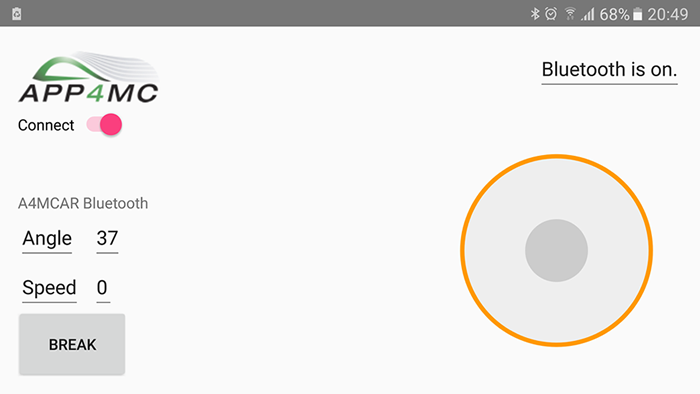
\includegraphics[scale=0.6]{content/images/androidapp.png}
	\caption{Android Application Developed for Driving A4MCAR Remotely}
	\label{fig:androidapp}
\end{figure}
\begin{figure}[!ht]
	\centering
	\captionsetup{justification=centering}
	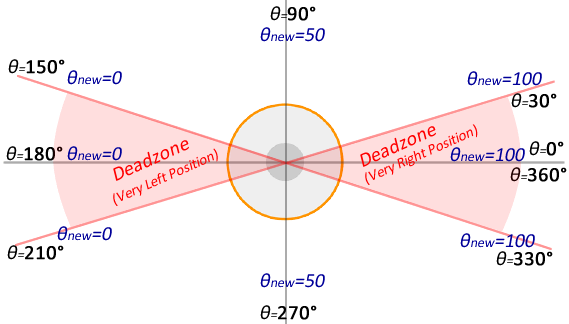
\includegraphics[scale=0.6]{content/images/joystickpie.png}
	\caption{Joystick angle transformation to construct driving command}
	\label{fig:joystickpie}
\end{figure}

Using the joystick illustration given in a Cartesian coordinate system, the angles that are generated by the joystick library itself $\theta$ (0 to 360 degrees) have been converted to the angles for the driving command format $\theta\textsubscript{new}$ (0 to 100). Although the transformations are made to the values from 0 to 100, later on this is reduced to the values from 0 to 99 in order to get rid of the 3-digit format which is not accepted by the command parser written in the low-level module side.

As it is clearly shown in the Figure \ref{fig:joystickpie}, there are certain dead zone regions on the joystick which are not taken into account in the transformation for the sake of the comfort of the users. While the transformed angle $\theta\textsubscript{new}$ is  constant in the dead-zone regions, a few equations have been used in order to handle the mapping of angles in the remaining regions:
\begin{itemize}
	\item If the angle is between 30 degrees and 150 degrees, the transformed new angle is calculated using the following:
	\begin{equation}
	\theta\textsubscript{new}=\left(1 - \frac{\theta - 30}{120}\right) 100
	\end{equation}
	\item If the angle is between 210 degrees and 330 degrees, the transformed new angle is calculated using the following:
	\begin{equation}
	\theta\textsubscript{new}=\left(\frac{\theta - 210}{120}\right) 100
	\end{equation} 
\end{itemize}
After the calculations, with the current gear setup the data is sent to the low-level module using the bluetooth functionality of the Android application.
%%% CHAPTER A4MCAR ------------------------------------end----


%%% CHAPTER Information Tracing and System Management --------begin----
\chapter{Information Tracing and System Management}
\section{Introduction}
After the distributed multi-core system is developed and defined, the evaluations regarding different software distributions are needed in order to parallelize the system efficiently. For that purpose, one should know how to manage the multi-core system. While managing the system is quite important to maintain and properly optimize the system to its full capabilities, one requires information regarding the system itself in order to achieve this optimization. As an example, the textbook methodology of extracting useful information from a software is to analyze online and offline trace of the system. 

In order to obtain information regarding a software such as number of instructions, how tasks are scheduled, timing details regarding tasks, core frequencies, energy consumption rates, the following techniques are mostly used:
\begin{itemize}
	\item \textbf{Static Binary Analysis:} Static binary analysis is a reverse engineering methodology that helps in finding errors in code such as the errors that involve non-determinism \cite{staticanalysisPRE}. It is essentially analyzing the binaries that are created from C and C++ programs to have another approach to traditional error finding methodologies such as testing and code inspection \cite{staticanalysisPRE}. It is important to keep in mind that in the static binary analysis, the program is not executed \cite{dynamicanalysisphd}. Therefore, the information regarding execution and timing are not provided while the instruction information could be extracted. However, it should be noted that some processor or platform specific tools can estimate the timing based on the number of instructions and the processor information. With the static binary analysis, the disassembly information which is the list of all the instructions could be observed. With the help of the binary analyzer tools, detailed information on number of function calls, nesting, and cyclic complexity could be observed \cite{staticvsdynamicanalysis}. %cyclomatic complexity.
	%this is simply observing disassembly
	\item \textbf{Profiling (Dynamic Analysis):}
	Dynamic analysis, also called profiling, is the methodology of analyzing the program by considering its execution in contrast to the static binary analysis \cite{dynamicanalysisphd}. Dynamic analysis is often done by using tools and it is done in order to get information of how a program is executed on a real or virtual processor \cite{staticvsdynamicanalysis}. While dynamic analysis is quite useful for identifying vulnerabilities in a runtime environment and obtaining information such as timing of execution, it can not guarantee the full test coverage of the source code \cite{staticvsdynamicanalysis}. Using dynamic binary instrumentation (DBI) tools for Linux platform this way, one can obtain information such as CPU time, execution times, memory and I/O of a program \cite{dynamicanalysisphd}. 
	\item \textbf{Tracing:} Tracing is a methodology which is often mixed with profiling. According to IPM \cite{IPM}, a trace records the chronological information of the execution of a program or a system via logging the the execution with timestamps, whereas a profile is the collection of performance events and timings for a program's execution as a whole. Therefore, it can be said that the scheduling of an Operating system could be analyzed with the help of tracing. 
	
	The A4MCAR involves tracing features that are not only supplied by Linux tools but are also developed within the project. It can be generalized that online tracing is a type of tracing that is done while the program is being executed using buffered logs while offline tracing is done after the program has executed using the entire logs. Regarding this information, it can be said that the developed tracing features are created for online tracing in A4MCAR while the existing tooling is used for offline tracing. The following sections consist of the information regarding tracing developments as well as the tooling support regarding tracing a Linux system.
	\item \textbf{System Monitoring:} Unlike static binary analysis and profiling, system monitoring \cite{systemmonitoring} is done within the entire system and it is used for obtaining useful information regarding the system performance as a whole. Operating systems (especially Linux platform) usually have system logs which could be observed via system monitoring in order to extract useful information regarding the system performance. Speaking for A4MCAR, the performance values such as core frequency and core utilization information are extracted using system monitoring.
	%We did this with psutil, also proc folder
\end{itemize}

%Here comes our motivations
%What kind of information needed?
%Why?
%In APP4MC
%Why do we do this?
%In both low and hight level modules
%This chapter will involve....
Low-level and high-level modules of A4MCAR requires several information. To start with, in order to model the software system of both modules with A4MCAR, the number of instructions, task iteration periods, and if exists event occurrance types are needed. This could be achieved by using static binary analysis method in the low-level module due to the fact that XTA tool can estimate instructions, timing, and path from the static binary analysis. The information of number of instructions and periods are obtained from the high-level module Linux platform by using tools that perform profiling. Although using a static binary analysis tool is possible, using a profiler tool was selected as the option for easement of the process. Secondly, system monitoring is needed in both of the modules. While the system monitoring is done using registers in the memory for the low-level module, it is achieved by using Linux kernel tools in high-level module. System monitoring in A4MCAR is essentially needed in order to obtain core utilization percentages, live CPU frequency and active core count. Finally, the profiling and tracing of the programs of the high-level module is needed in order to evaluate parallelization performance and visualize how processes are scheduled. The data that are obtained from profiling and tracing involve slack time, execution times, start and end times.

In this chapter, the aforementioned techniques for system analysis will be discussed with the emphasis of their applicability on a real distributed multi-core system that involves elements from a low-level multi-core micro-controller and a high-level single board computer that is running on x86/Linux platform in order to elaborate  modeling, managing, profiling, tracing of systems and evaluation of various software distributions.

\section{Low-Level Module Information Tracing and System Management}
\subsection{Static Binary Analysis via XTA}
XMOS Timing Analyzer (XTA) \cite{xtamanual} is a tool that comes with xTIMEcomposer platform which is used for analyzing the timing and the execution details of the multi-tasked software that are developed using XMOS boards and processors \cite{xtamanual}. The tool is able to measure shortest and longest time required to execute a section of code by analyzing the binary file. Thus, the code is not executed in order to be analyzed. Furthermore, it is also able to check the minimum and maximum number of instructions required to execute a section of the code.  A screenshot from the XTA tool is given in the Figure \ref{fig:xtass}.

\begin{figure}[!ht]
	\centering
	\captionsetup{justification=centering}
	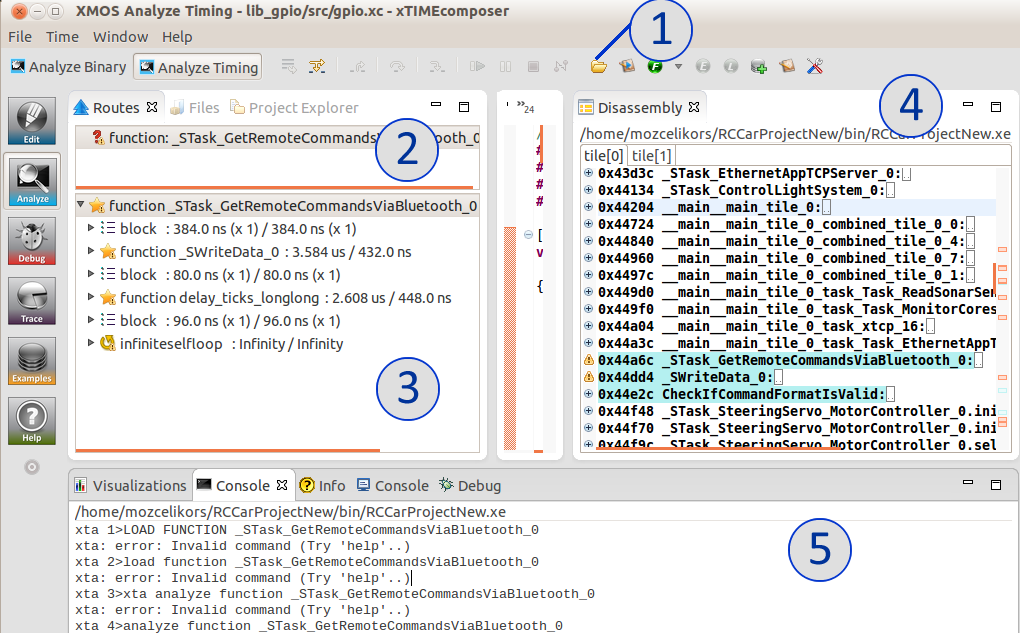
\includegraphics[width=\textwidth]{content/images/xtass.png}
	\caption{XMOS Timing Analyzer (XTA) screenshot}
	\label{fig:xtass}
\end{figure}

Once the code is written and built in xTIMEcomposer platform, a binary file is generated with the extension .XE. By loading this binary file using XTA, the timing analysis could be performed. In order to load the binary to XTA, "Load Binary" button (shown as 1 in the Figure \ref{fig:xtass}) should be pressed. Once the binary is loaded, the Disassembly window (shown as 4) appears which shows all the runnables that are automatically detected from the binary. Using the disassembly window, the instructions that are used in runnables could be seen. 

XTA tool is also able to work with specific commands by using the XTA console (shown as 5). Using the specific commands taken from XTA manual \cite{xtamanual}, timing analysis could be done easily. In order to start timing analysis, an execution path should be defined. The execution path could be determined analyzed using the following possible ways \cite{xtamanual}:
\newpage
\begin{itemize}
	\item Via placing end points into the code using compiler directive \texttt{\#}pragma as shown in the Listing \ref{lst_xtaendpoints}.
	\lstinputlisting[caption=Placing end points in xC code to define execution path , label=lst_xtaendpoints, style=xc]{content/listings/lst_xtaendpoints.txt}
	The timing analysis between two endpoints could be started by entering the following command to the XTA console:
	\begin{lstlisting}[style=xc]
	analyze endpoints start_endpoint1 stop_endpoint1
	\end{lstlisting}
	\item A function or a runnable with the name "Function\texttt{\_}Name" could be analyzed from its starting point to its return point by using the following command:
	\begin{lstlisting}[style=xc]
	analyze function Function_Name
	\end{lstlisting}
	\item Finally, loops can be analyzed using XTA. The way a loop is defined is either setting a loop point from the editor or defining an endpoint inside loop. A loop point having and end point "looppoint" can be analyzed using the following command in the XTA console:
	\begin{lstlisting}[style=xc]
		analyze loop looppoint
	\end{lstlisting}
\end{itemize}

The entire code could be modified in the aforementioned fashion in order to do a timing analysis to all of the runnables of the software system. One can set up timing constraints to make sure every dead line is matched \cite{xtamanual}. Once the timing analysis starts, the selected route, i.e. a function, a loop, or a route between two endpoints are shown in the Routes window (shown as 2 in the Figure \ref{fig:xtass}). The selected route is shown in blocks in another window which is shown as 3 in the figure. Here, it is seen that the best case execution time and the worst case execution time of each block is estimated. As an example, for the WriteData function, the best case execution time is estimated to be 3.584 microseconds, whereas the worst case execution time is 432 nanoseconds. Further information that is provided by XTA regarding timing analysis is given in the Figure \ref{fig:xtafurther}. As it is seen in the figure, what kind of timing paths could have been taken for the function can be visualized using the Visualizations window. Furthermore, information such as thread cycles, number of instructions, number of Fnops, and number of paths are also shown.

\begin{figure}[!ht]
	\centering
	\captionsetup{justification=centering}
	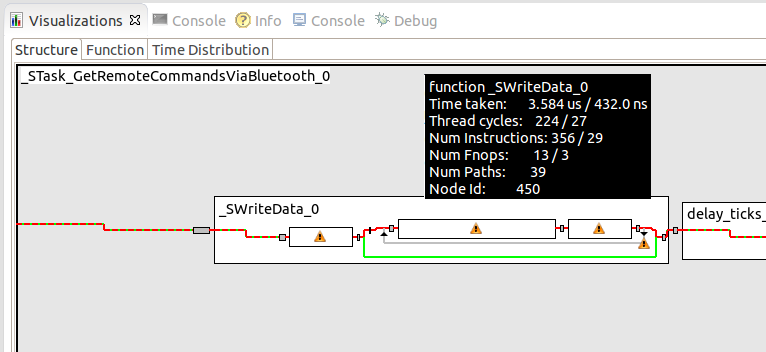
\includegraphics[width=\textwidth]{content/images/xtafurther.png}
	\caption{XTA Visualizations window with further information}
	\label{fig:xtafurther}
\end{figure}

For the software that is developed for the low-level module of the A4MCAR, for modeling purposes in APP4MC  the number of instructions are obtained for almost every runnable and event by using aforementioned techniques. For the events, the technique of defining endpoints is used, whereas for the runnables the function analysis is used. However, due to the non-determisim in the some of the branch instructions and code sections that are related to hardware communication, some sections in many runnables were not able to be analyzed properly and returned the "Unresolved" error. In order to get rid of this error, following techniques are used:

\begin{itemize}
	\item The "Unresolved" error occurs usually when XTA can not resolve a branch instruction whose branch target is unknown \cite{xtamanual}. In order to get rid of this issue, trace of the system should be printed and branch instruction target should be pointed manually. The details of how this is done is given in the XTA manual \cite{xtamanual}. By using this technique, some of the "Unresolved" errors were resolved and number of instructions of those runnables were found.

	\item When the technique above failed to work because of memory instructions such as memset and infinite loops, the number of instructions are gathered by counting the instructions from Disassembly window. Although this technique is time consuming and error-prone, it is assumed that the gathered information is close to the real number of instructions. Additionally, APP4MC partitioning and mapping accuracy would not change drastically if the gathered information is not exact. 
\end{itemize}

In the Section 6, gathered information along with its implications will be discussed.
\subsection{Information Tracing via APP4MC}
Some text \\
\subsection{Distribution of Tasks to Cores}
In a properly utilized parallel system, gathered information are used in order to find which software distribution is the most efficient. Here, the software distribution refers to the mapping stage, which is the distribution of the tasks that result from partitioning to the cores.

In xTIMEcomposer platform, task mapping is done easily with the capabilities of the xC programming language. Since xCORE provides a multi-core platform, using the cores for different tasks can be achieved by using simple statements. Although this is introduced in Section 4, some of the information will be summarized for completeness sake. In XMOS, placement of a function into a core is done by using "par" statement. In the main block of a software, "par" statement can be used in order to create several tasks in parallel. Additionaly, using global interface variables, one can handle the inter-task communication between two parellel tasks.

As opposed to the Listing \ref{lst_howtasksconnectxc}, a simple example would help one better understand how this works using xC:

\begin{lstlisting}[style=xc]
int main(void)
{
	interface my_interface i1;
	par
	{
		on tile[0].core[2] :  Task1 (i1);
		on tile[1].core[3] :  Task2 (i2);
	}
}
\end{lstlisting}

The given code is a basic example of using xC functionality to do a task mapping. The parallel block in the code could be given as the Lines 4 through 8. It is seen that the "Task1" is pinned to the core 2 of tile 0, whereas the "Task2" is pinned to the core 3 of the tile 1. Furthermore, a global interface of type "my\texttt{\_}interface" having the name i1 is declared in the Line 3. This interface handles the communication between the tasks "Task1" and "Task2". As mentioned, the hardware realizes the interface by using the xCONNECT switches to construct a bridge between tiles and cores. Additionally, it should be noted that unlike Raspberry Pi, the tasks are distributed to cores during the reconfiguration in a xC program, i.e where a Task is located can not be changed during run-time due to the nature of xCORE and due to the fact that hardware availability differs from tile to tile \cite{xmosprogrguide}.

By using the aforementioned technique, all the low-level module tasks are distributed to cores at the build-time. 

\subsection{System Monitoring in xCORE}
How cores of the system is monitored in xCORE is discussed in the Section 4. For the sake of completeness, this subsection is dedicated to reminding what is discussed in the Section 4, "Core and Tile Monitoring" subsection. System monitoring is done by polling a system register and finding out if that core is busy or idle at that moment. Referring back to the Listing  \ref{lst_coremonitoring}, how this is achieved could be better understood.

Besides the implemented core monitoring task, XMOS features several more means to monitor the system. First, system could be monitored at build-time using the XTA tool Binary window, Resource Usage tab. In the Figure given in \ref{fig:binaryresourceusage}, it is seen that the information regarding stack memory, program memory, free memory, cores, timers, and channels could be observed in one window using XTA Binary. Another mean to monitor the system is provided by a function called "debug\texttt{\_}printf". As the name of the function suggests, it is essentially a "printf" function to observe your variables. However, "debug\texttt{\_}printf" is a function that does not interrupt inter-process communication and that does not block cores while printing so that developers can monitor without having to worry about so much overhead \cite{xmosprogrguide}.

\begin{figure}[!ht]
	\centering
	\captionsetup{justification=centering}
	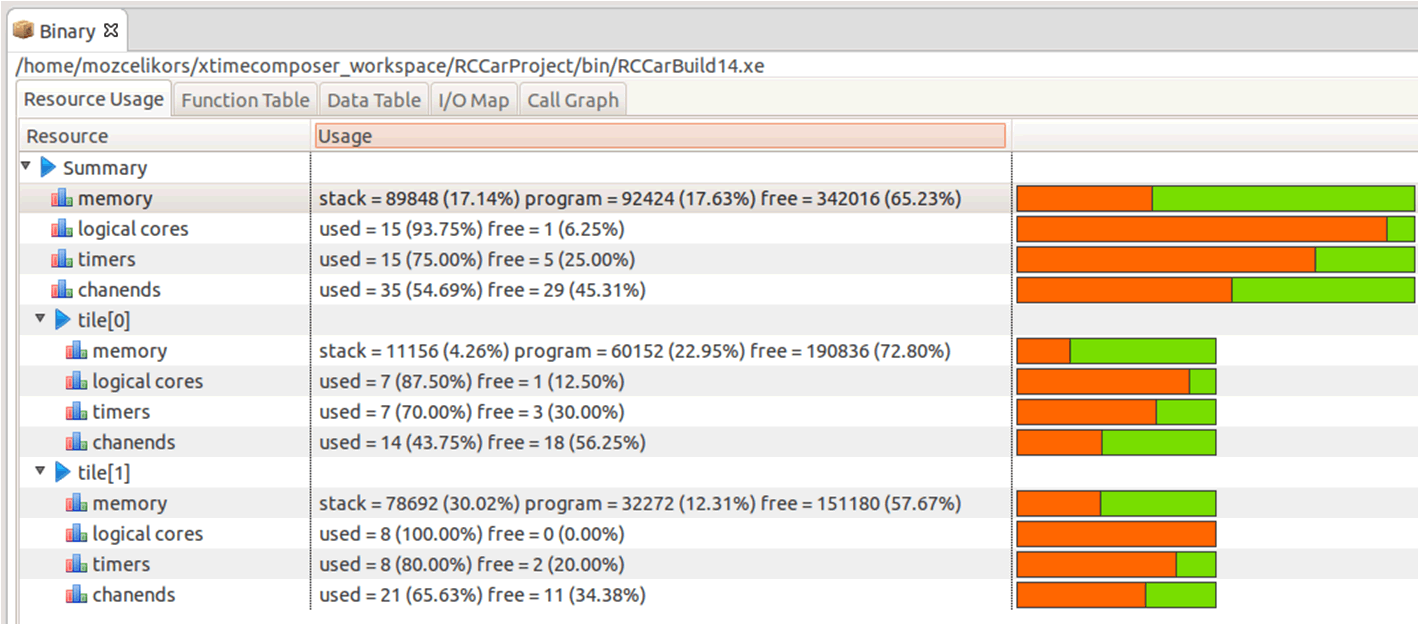
\includegraphics[width=\textwidth]{content/images/binaryresourceusage.png}
	\caption{XTA Binary Resource Usage}
	\label{fig:binaryresourceusage}
\end{figure}

Using the "debug\texttt{\_}printf" function, xC-specific tools, a function has been created that helps to find out which function refers to which core. The reason this information is important is because the core ids that are referred with the "par" statements are not the same ids of the core usage implemention. The same issue holds true for the tile ids, as well. By using the following listing, this information could be monitored at run-time:

\begin{lstlisting}[style=xc]
	int PrintCoreAndTileInformation(char * Function_Name)
	{
		debug_printf("Starting %s task on core ID %d on tile %x\n", Function_Name, 	get_logical_core_id(), get_local_tile_id());
		return 1;
	}
\end{lstlisting}

Here, the get\texttt{\_}logical\texttt{\_}core\texttt{\_}id() is the function to get the real core id from system registers, whereas the get\texttt{\_}local\texttt{\_}tile\texttt{\_}id() function returns the real tile id. This way, we make sure which task uses how many percentage of the core. Once every task is manipulated so that they use this function while the core monitoring is running, system monitoring could be done easily by observing the Console. An example output of the Console from final version of the low-level module software is given with the Figure \ref{fig:finalmonitoring}. It is seen that the core IDs for every task is given and then the core utilization percentages are listed for cores 0 through 7 for each tile.

\begin{figure}[!ht]
	\centering
	\captionsetup{justification=centering}
	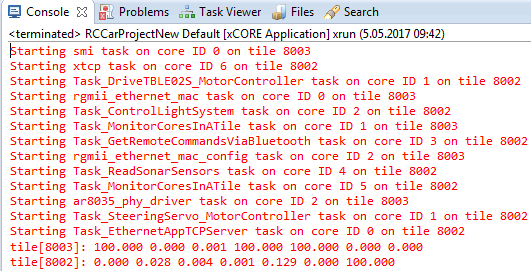
\includegraphics[width=\textwidth]{content/images/finalmonitoring.png}
	\caption{System monitoring implemented on xCORE}
	\label{fig:finalmonitoring}
\end{figure}

%%Onceki sectiona ek olarak
%% core_monitoring.xc den bahset
\subsection{Discovering Energy Consumption Features}
Some text \\
\section{High-Level Module Information Tracing and System Management}

\subsection{Obtaining Information}
\subsubsection{Binary Analysis of Instructions}
% perf stat, objdump, dis
Some text \\
\subsubsection{Process Management, Monitoring, and Profiling}
% top (incl threads), ps,getting pid, getting killing processes using ps, proc folder, psutil
%valgrind etc. profiling
% starting, killing a process, ProcessKill.sh ProcessStart.sh, AppMonitor.sh
Some text \\
\subsubsection{System Monitoring for Linux Platform}
%proc folder, psutil, top, ps
Some text \\
\subsubsection{Tracing the System to Obtain Scheduling Information}
% perf record, trace-cmd, kernelshark, perf w/babeltrace, CTF, lttng, TraceCompass
Some text \\
\begin{figure}[!ht]
	\centering
	\captionsetup{justification=centering}
	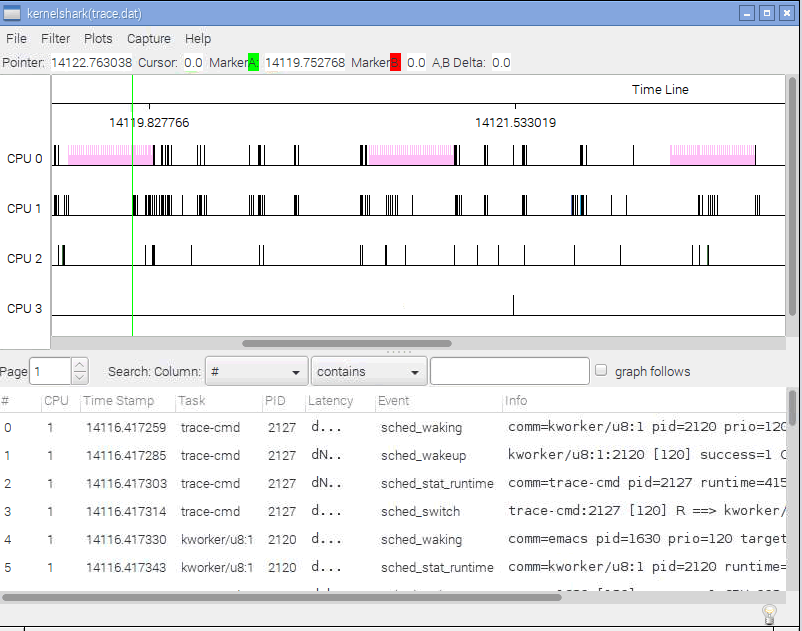
\includegraphics[scale=0.55]{content/images/kernelshark.png}
	\caption{Kernelshark running on Linux (Raspbian) OS}
	\label{fig:kernelshark}
\end{figure}

\begin{figure}[!ht]
	\centering
	\captionsetup{justification=centering}
	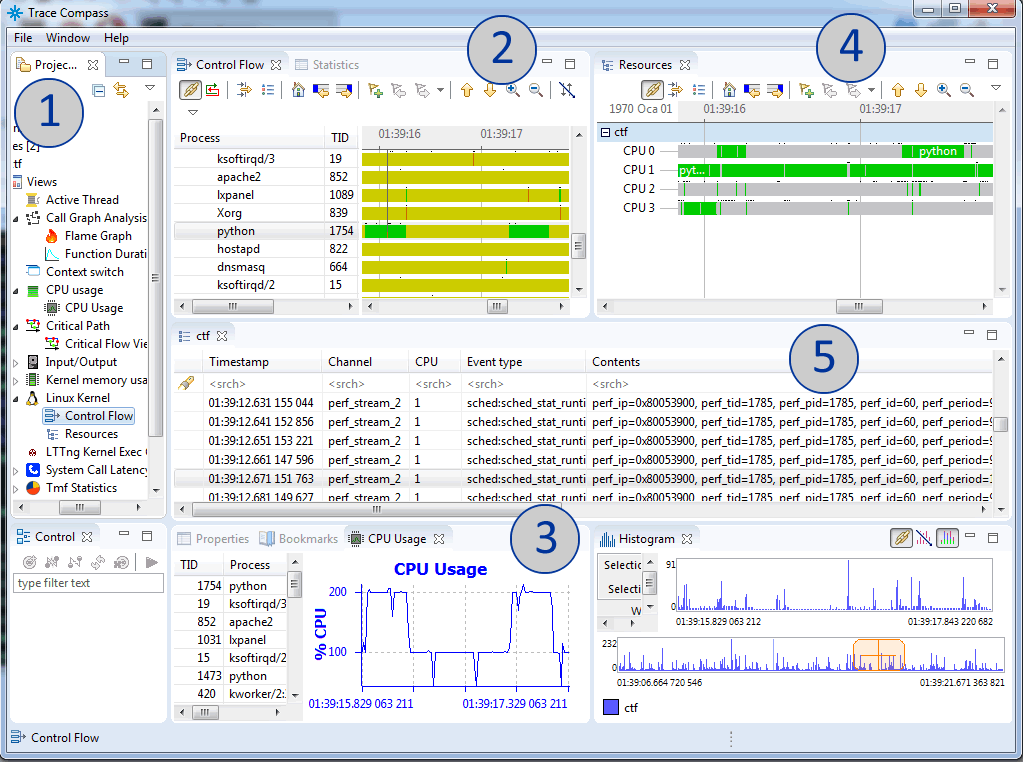
\includegraphics[scale=0.45]{content/images/tracecompass.png}
	\caption{Eclipse TraceCompass running on Windows}
	\label{fig:tracecompass}
\end{figure}

\subsection{Process Mapping}
% taskset, CorePlacer.sh
Some text \\
\subsection{Discovering Energy Consumption Features}
%cpufrequtils
Some text \\
\subsection{Online Timing Analysis Features in A4MCAR}
%whats implemented before in every app, and whats implemented in the touchscreen display (main process)
%Including formulas for avg.slack time and so on...
Some text \\

%%% CHAPTER Information Tracing and System Modeling --------end----
%%% CHAPTER Effective Parallelism Evaluation --------begin----
\chapter{Effective Parallelism Evaluation}
Some text \\
\section{Low-Level Module Parallelism} %in RCCAR
Some text \\
\subsection{System Model}
Some text \\
\subsection{Efficiency Model}
Some text \\
\subsection{Evaluation of Different Distributions}
Some text \\
%Give Everything in a table, which core mapped, period, execution time rougly, cpu core usage roughly.
%Also use data from TraceCompass

\begin{table}[h!]
	\begin{tabular}{|l|l|l|}
		\hline
		Name & Title & Year \\
		\hline
		\hline
		Philip K. Dick & Minority Report & 1956 \\
		\hline
	\end{tabular}
	\caption{Einfache Tabelle}
	\label{properties_coremonitoring}
\end{table}
\subsection{Results from APP4MC Distribution}
Some text \\
\section{High-Level Module Parallelism}
Some text \\
\subsection{System Model}
Some text \\
\subsection{Efficiency Model}
Some text \\
\subsection{Evaluation of Different Distributions}
Some text \\
\subsection{Results from APP4MC Distribution}
Some text \\
%Distributed system and embedded systems characteristics.... scalability etc.. real-time system.
%Also description of our systems characteristics.

%x APPSTACLE emphasis
%Quote:
%The main benefit for having release, start, (preemption), end, and deadline values is deriving efficiency. For each task instance, you can calculate e.g. the slack time, that indicates how much time is left before its next execution. The higher the slack time is, the better was its execution. Different scenarios and different tasks have different profiling results (slack time is just one of them) and their investigation leads to a precise assessment of software distribution!
%(Maybe also involve deadline misses..)

%the period usually is the deadline. as soon as execution time exceeds this, you must indicate a “deadline miss” it can lead to system failure or even cause (in the automotive domain) person harm. Think of a break application that must react within e.g. 1ms to ensure accurate braking.
%To answer your question: it is ok, but you must indicate the deadline miss
%you should ‘design’ (since you do not have any timing requirements) the periods in a way that they should meet deadlines
%f you want to show that unser a certain period definition, deadline misses definitely occure (e.g. sequential execution) than you can, for sure, design the periods in that way
% you can measure different scenarios (periods) though (i recommend that)

%Design of rpi apps and timing for real-time scheduling...
%Formulas and how the display timing designed.
%How deadlines designed with periods conforming to parallel distribution

%Linux OS overheads + App Timing additions overhead..


%Give scheduling image.. and explain..

%Real-time Scheduling in Linux?????
%time.time (real time) vs time.clock (processor time) (does not count cpu sleeps)

%Overall mean slack time -> longer means distribution is better.
% Core execution times should be same but Response times  (= GETs ) will slightly differ.
%Why dont we have IPT? which causes Response times = GETs

%Different measurements -> scenerios -> results evaluation using kernelshark, lttng AND TraceCompass!!! and other tools. (also include image processing app in some scenerios)

%Online efficiency calculation using rpi and offline distribution analysis.

% Real-time EMPHASIS REALLY IMPORTANT. MAKE A CHAPTER ON THAT

%Why real-time computing not supported in ARM architecture, especially Raspberry Pi ? (search this!!)

% Thread analizini de yapalim
%top -H -p <pid> or ps -T -p <pid>
%Clock speed > Power

%Problems measuring efficiency using slack time with Rpi:
%There needs to be a dynamic sleep time(period-exectime)
%time.timeshould be used instead of time.clock()

%x DVFS Dynamic Voltage and Frequency Scaling


%%% CHAPTER Effective Parallelism Evaluation --------end----
%%% CHAPTER Conclusion ----------------------------begin----
\chapter{About APPSTACLE Project}
\chapter{Conclusion}

%%% CHAPTER Conclusion ------------------------------end----
	%\chapter{Wissenschaftliches Arbeiten}
	%	\section{Vorgehen}

Grunds�tzlich ist es wichtig, das die komplette Arbeit einen "`roten Faden"' besitzt und entsprechend strukturiert ist. 

Arbeitsschritte beim wissenschaftlichen Arbeiten:
\begin{itemize}
	\item Wahl des Themas und erste Konkretisierung
	\item Zeitplanung
	\item Informationsbeschaffung
	\item Literaturrecherche
	\item Informationsaufnahme und -verdichtung
	\item Lesen, exzerpieren, archivieren, systematisieren
	\item Informationsvermittlung
	\item Erstellen einer Ausarbeitung
	\item Erstellen einer Pr�sentation
\end{itemize}

%********************** Bewertungskriterien *******************
\section{Bewertungskriterien}

\subsection{Bewertung schriftlicher Arbeiten}

\begin{enumerate}
	\item Umfang und Form
	\begin{itemize}
		\item ca. 40 inhaltliche Seiten bei Projektarbeiten und ca. 80 bei Bachelor- und Diplomarbeiten  
		\item korrekte Orthographie, Interpunktion, Grammatik und Stil der Formulierungen
		\item korrekte, vollst�ndige und konsistente Zitierweise
		\item Trennung von Beschreibung und Bewertung
		\item kriteriengeleitete Auswahl
	\end{itemize}
	\item Allgemeine Verst�ndlichkeit
	\begin{itemize}
		\item knapper, informativer und verst�ndlicher Titel 
		\item folgerichtiges, klares und m�glichst redundanzfreies Inhaltsverzeichnis
		\item einf�hrender �berblick 
		\item kurze Zusammenfassung(en)
		\item verst�ndliche und konsistente Abbildungen 
		\item vollst�ndiges Quellenverzeichnis
		\item verst�ndliches und konsistentes Layout (z.B. kursiv zur Hervorhebung, fett zur Einf�hrung neuer Fachtermini,  Courier f�r Code und Pseudocode)
		\item Koh�renz (Zusammenhang zwischen den Abschnitten)
		\item Veranschaulichung mit Beispielen 
	\end{itemize}
	\item Fachspezifische Verst�ndlichkeit
	\begin{itemize}
		\item korrekte und konsistente Terminologie 
		\item Informatikwissen f�r Informatiker verst�ndlich aufbereiten (nicht zu viel Details ($\rightarrow$ Referenzen), aber soviel wie n�tig)
		\item folgerichtige Sequenzierung (roter Faden) 
	\end{itemize}
	\item Tiefe und Anspruch
	\begin{itemize}
		\item begrifflicher Gehalt (insbesondere ausreichende Operationalisierung) 
		\item methodischer Gehalt (insbesondere korrekte Anwendung der Fachmethoden) 
		\item technischer Gehalt (z.B. Auswahl der verwendeten Standards oder Werkzeuge) 
		\item	Abstraktionsgrad (Verallgemeinerung auf andere Dom�nen)
	\end{itemize}
\end{enumerate}



\subsection{Bewertung von Pr�sentationen im Kolloquium}

\begin{itemize}
		\item Struktur, Sequenzierung (roter Faden)
		\item sinnvolle Medienwahl (Folien, Wandtafel, Beamer ...) 
		\item akustischer und sprachlicher Ausdruck 
		\item visuelle Verst�ndlichkeit (Folien- und Wandtafeldarstellungen) 
		\item Ausrichtung auf den Zuh�rerkreis (Zielgruppe: oberes Management)
		\item Einhaltung der Zeitvorgabe (30 Minuten inkl. Demonstration und Fragen)
		\item freie Rede
		\item kompetente Beantwortung von Fragen
	\end{itemize}


%********************** Vortragstipps *******************
\section{Vortragstipps}
\begin{itemize}
	\item Stellen Sie sich und Ihr Thema zu Beginn vor und ordnen es in den Kontext ein.
	\item Das Wesentliche aus der zu bearbeitenden Literatur exzerpieren, ohne die gesamte Arbeit vorzutragen; unwichtige Details auslassen.
	\item Kritische Distanz zum Thema wahren: eigene Beurteilung des Stoffes versuchen (z.B. Eignung und m�gliche Anwendungsgebiete bestimmter Verfahren, Vor- und Nachteile von Systemen).
	\item Rede so vorbereiten, dass Teile bei Zeitnot weggelassen werden k�nnen ($\rightarrow$ Bilder). Ein Bild sagt mehr als 1000 Worte.
	\item Zeit f�r Fragen und Diskussion ber�cksichtigen ($\rightarrow$ Planung).
	\item Auf Fragen aus dem Publikum w�hrend des Vortrags immer eingehen, nie abweisend oder unwirsch reagieren. Falls die Fragen �berhandnehmen und die Zeit f�r unverzichtbare (!) Teile des Vortrags knapp wird, sollte man dies den Zuh�renden mitteilen und sie darum bitten, Fragen m�glichst erst nach dem Vortrag zu stellen.
	\item Den Text des Vortrag nicht ablesen oder auswendig herunterbeten: selbst eine manchmal stockend oder mit Pausen gehaltene freie Rede bringt den Zuh�renden mehr.
	\item Nicht nur vorlesen, was auf den Folien steht: zus�tzliche Informationen und Erl�uterungen sind zum Verst�ndnis �u�erst wichtig.
	\item Merkzettel vorbereiten, auf denen stichwortartig vermerkt ist, was man w�hrend des Vortrags erz�hlen mochte. Wichtig f�r die Momente im Vortrag, in denen man selbst den Faden verliert und nachsehen muss, was man als n�chstes erz�hlen wollte.
	\item Es ist meistens sehr hilfreich, die ersten Satze des Vortrags auswendig zu lernen, da dann der Einstieg wesentlich leichter ist.
	\item Der vollst�ndige Vortrag mit den fertigen Folien sollte mindestens einmal (m�glichst vor kritischem Publikum, nur im Notfall allein) im vor aus ge�bt werden.
	\item Beim Vortrag den Blick der Zuh�renden durch Zeigen auf Texte und Graphiken fuhren. Vorsicht: dabei nicht vom Publikum abwendet und nur noch zur Leinwand sprechen!
	\item Beim Reden �fter Blickkontakt zu den Zuh�renden herstellen. Laut reden. Redepausen machen. Nicht zu schnell reden. "`�hm"'-Laute vermeiden.
	\item Sprechen Sie mit Betonung und erm�den die Zuh�rer nicht durch monotone Sprechweise.
\end{itemize}
	%\chapter{Arbeiten mit \LaTeX}
	%	\section{Quelltext und Bilder}

Das Einbinden von Quelltexten ist in \LaTeX mit dem Listings-Paket sehr komfortabel m�glich. Es lassen sich \texttt{verschiedene} Sprachen \textit{definieren} und man kann aktiv in die Darstellung der einzelnen Sprachelemente \textbf{eingreifen}.

%************** XML ******************
\subsection{XML}
Beispiel f�r XML-Code siehe Quelltext \ref{lst_xml_code}

\lstinputlisting[caption=Beispiel f�r XML-Code, label=lst_xml_code, style=xml]{content/listings/xml_code.xml}


%************** JAVA ******************
\subsection{JAVA}
Beispiel f�r Java-Code siehe Quelltext \ref{lst_java_code}

\lstinputlisting[caption=Beispiel f�r Java-Code, label=lst_java_code, style=java]{content/listings/java_code.java}


%************** BILDER ******************
\subsection{Bilder}
Beispiel um ein Bild einzuf�gen siehe Abbildung \ref{fig:FB4Bild}

\begin{figure}[htb]
	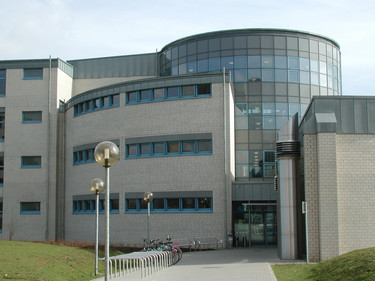
\includegraphics{content/images/52_Foto_FHDortmund_Gebaeude.jpg}
	\caption{Geb�ude des FB4}
	\label{fig:FB4Bild}
\end{figure}


%************** FORMELN ******************
\subsection{Formeln}
Einfache Formeln oder einzelne mathematische Symbole k�nnen durch das Dollar-Zeichen \$ eingebunden werden: \$ Formel \$. Eine so erstellte Formel k�nnte folgenderma�en aussehen:
\begin{center}
	$X(z) = \sum_{n=-\infty}^\infty ( x[n]  * r^{-n} ) * e^{-j\omega n}$ \\
\end{center}

Werden in dem Dokument viele Formeln verwendet und soll bei Bedarf noch einmal darauf zur�ckgegriffen werden k�nnen, macht es Sinn Formeln zu nummerieren. Dazu m�ssen Formeln folgenderma�en eingebunden werden:\\

\textbackslash begin\{equation\textbraceright \\
	\noindent\hspace*{10mm} Hier die Formel\\
\textbackslash end\{equation\textbraceright

Das Ergebnis k�nnte so aussehen:
\begin{equation}
		t-t_{0}=\sqrt{\frac{l}{g}}\int_{0}^{\varphi}{\frac{d\psi}{\sqrt{1-k^{2}\sin^{2} {\psi}}}} = \sqrt{\frac{l}{g}} F(k,\varphi)
\end{equation}
	%	\section{Zeichnungen}

Die folgenden Zeichnungen wurden mit den \LaTeX -Zusatzpaketen pgf und tikz erstellt. Sie stellen sehr m�chtige Werkzeuge zur Verf�gung um Diagramme und Grafiken aller Art zu erstellen. Die Ergebnisse sind professionell und k�nnen, falls n�tig, mit wenig Aufwand ge�ndert werden. Es erfordert nat�rlich eine gewisse Einarbeitung, aber diese wird durch die Resultate schnell wieder aufgewogen.
Eine umfangreiche Anleitung mit vielen weiteren Beispielen findet sich auf \\ \href{http://www.ctan.org/tex-archive/graphics/pgf/base/doc/generic/pgf/pgfmanual.pdf}{http://www.ctan.org/tex-archive/graphics/pgf/base/doc/generic/pgf/pgfmanual.pdf} \\

Es folgen einige Beispiele.


%********************** Zustandsdiagramm *******************
\subsection{Zustandsdiagramm}

Das Zustandsdiagramm (englisch: state diagram) der UML ist eine der dreizehn Diagrammarten dieser Modellierungssprache f�r Software und andere Systeme. Es stellt einen endlichen Automaten in einer UML-Sonderform grafisch dar und wird benutzt, um entweder das Verhalten eines Systems oder die zul�ssige Nutzung der Schnittstelle eines Systems zu spezifizieren.

\begin{figure}[H]
\begin{center}
	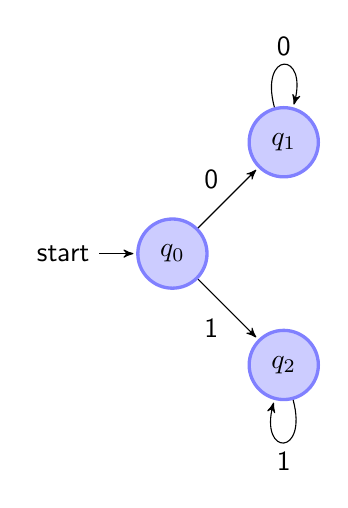
\begin{tikzpicture}[shorten >=1pt,node distance=2cm,on grid,>=stealth', every state/.style={draw=blue!50,very thick,fill=blue!20}]
		\node[state,initial] (q_0) {$q_0$};
		\node[state] (q_1) [above right=of q_0] {$q_1$};
		\node[state] (q_2) [below right=of q_0] {$q_2$};
		\path[->] (q_0) edge node [above left] {0} (q_1)
			edge node [below left] {1} (q_2)
			(q_1) edge [loop above] node {0} ()
			(q_2) edge [loop below] node {1} ();
	\end{tikzpicture}
	\caption{Zustandsdiagramm}
	\label{fig:zustandsdiagramm}
\end{center}
\end{figure}


%********************** Petrinetz *******************
\subsection{Petrinetz}
Ein Petri-Netz ist ein mathematisches Modell von nebenl�ufigen Systemen. Es ist eine formale Methode der Modellierung von Systemen bzw. Transformationsprozessen. Die urspr�ngliche Form der Petri-Netze nennt man auch Bedingungs- oder Ereignisnetz. Petri-Netze wurden durch Carl Adam Petri in den 1960er Jahren definiert. Sie verallgemeinern wegen der F�higkeit, nebenl�ufige Ereignisse  darzustellen, die Automatentheorie.

\begin{figure}[H]
\begin{center}
		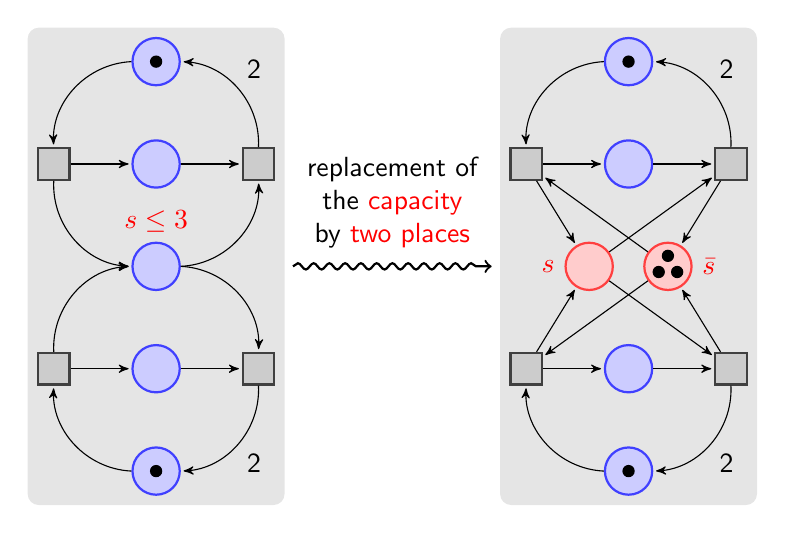
\begin{tikzpicture}
			[node distance=1.3cm,on grid,>=stealth',bend angle=45,auto,
			every place/.style= {minimum size=6mm,thick,draw=blue!75,fill=blue!20},
			every transition/.style={thick,draw=black!75,fill=black!20},
			red place/.style= {place,draw=red!75,fill=red!20},
			every label/.style= {red}]
			\node [place,tokens=1] (w1) {};
			\node [place] (c1) [below=of w1] {};
			\node [place] (s) [below=of c1,label=above:$s\le 3$] {};
			\node [place] (c2) [below=of s] {};
			\node [place,tokens=1] (w2) [below=of c2] {};
			\node [transition] (e1) [left=of c1] {}
			edge [pre,bend left] (w1)
			edge [post,bend right] (s)
			edge [post] (c1);
			\node [transition] (e2) [left=of c2] {}
			edge [pre,bend right] (w2)
			edge [post,bend left] (s)
			edge [post] (c2);
			\node [transition] (l1) [right=of c1] {}
			edge [pre] (c1)
			edge [pre,bend left] (s)
			edge [post,bend right] node[swap] {2} (w1);
			\node [transition] (l2) [right=of c2] {}
			edge [pre] (c2)
			edge [pre,bend right] (s)
			edge [post,bend left] node {2} (w2);
			\begin{scope}[xshift=6cm]
			\node [place,tokens=1] (w1') {};
			\node [place] (c1') [below=of w1'] {};
			\node [red place] (s1') [below=of c1',xshift=-5mm]
			[label=left:$s$] {};
			\node [red place,tokens=3] (s2') [below=of c1',xshift=5mm]
			[label=right:$\bar s$] {};
			\node [place] (c2') [below=of s1',xshift=5mm] {};
			\node [place,tokens=1] (w2') [below=of c2'] {};
			\node [transition] (e1') [left=of c1'] {}
			edge [pre,bend left] (w1')
			edge [post] (s1')
			edge [pre] (s2')
			edge [post] (c1');
			\node [transition] (e2') [left=of c2'] {}
			edge [pre,bend right] (w2')
			edge [post] (s1')
			edge [pre] (s2')
			edge [post] (c2');
			\node [transition] (l1') [right=of c1'] {}
			edge [pre] (c1')
			edge [pre] (s1')
			edge [post] (s2')
			edge [post,bend right] node[swap] {2} (w1');
			\node [transition] (l2') [right=of c2'] {}
			edge [pre] (c2')
			edge [pre] (s1')
			edge [post] (s2')
			edge [post,bend left] node {2} (w2');
			\end{scope}
			\begin{pgfonlayer}{background}
			\node (r1) [fill=black!10,rounded corners,fit=(w1)(w2)(e1)(e2)(l1)(l2)] {};
			\node (r2) [fill=black!10,rounded corners,fit=(w1')(w2')(e1')(e2')(l1')(l2')] {};
			\end{pgfonlayer}
			\draw [shorten >=1mm,-to,thick,decorate,
			decoration={snake,amplitude=.4mm,segment length=2mm,
			pre=moveto,pre length=1mm,post length=2mm}]
			(r1) -- (r2) node [above=1mm,midway,text width=3cm,text centered]
			{replacement of the \textcolor{red}{capacity} by \textcolor{red}{two places}};
		\end{tikzpicture}
	\caption{Petrinetz}
	\label{fig:petrinetz}
	\end{center}
\end{figure}



%********************** Graph *******************
\subsection{Graph}

Ein Graph besteht in der Graphentheorie anschaulich aus einer Menge von Punkten, zwischen denen Linien verlaufen. Die Punkte nennt man Knoten  oder Ecken, die Linien nennt man meist Kanten, manchmal auch B�gen. Auf die Form der Knoten und Kanten kommt es im allgemeinen dabei nicht an. Knoten und Kanten k�nnen auch mit Namen versehen sein, dann spricht man von einem benannten Graphen.

\begin{figure}[H]
	\begin{center}
	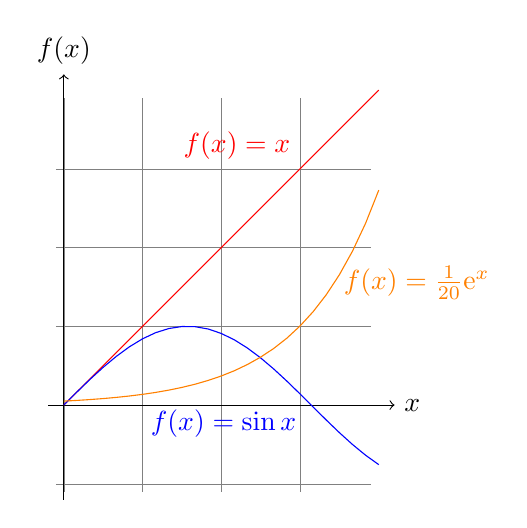
\begin{tikzpicture}[domain=0:4,label/.style={postaction={
	decorate,
	decoration={
		markings,
		mark=at position .75 with \node #1;}}}]
	\draw[very thin,color=gray] (-0.1,-1.1) grid (3.9,3.9);
	\draw[->] (-0.2,0) -- (4.2,0) node[right] {$x$};
	\draw[->] (0,-1.2) -- (0,4.2) node[above] {$f(x)$};
	\draw[red,label={[above left]{$f(x)=x$}}] plot (\x,\x);
	\draw[blue,label={[below left]{$f(x)=\sin x$}}] plot (\x,{sin(\x r)});
	\draw[orange,label={[right]{$f(x)= \frac{1}{20} \mathrm e^x$}}] plot (\x,{0.05*exp(\x)});
\end{tikzpicture}
	\caption{Graph}
	\label{fig:graph}
	\end{center}
\end{figure}

	%	%Tabellen%
\section{Tabellen}

Hier finden sich einige Beispiele f�r Tabellen und etwas Blindtext drumrum, damit sie nicht so verloren aussehen :)

Lorem ipsum dolor sit amet, consectetuer adipiscing elit. Aenean commodo ligula eget dolor. Aenean massa. Cum sociis natoque penatibus et magnis dis parturient montes, nascetur ridiculus mus. Donec quam felis, ultricies nec, pellentesque eu, pretium quis, sem. Nulla consequat massa quis enim. Donec pede justo, fringilla vel, aliquet nec, vulputate eget, arcu. In enim justo, rhoncus ut, imperdiet a, venenatis vitae, justo. Nullam dictum felis eu pede mollis pretium. Integer tincidunt. Cras dapibus. Vivamus elementum semper nisi. Aenean vulputate eleifend tellus. Aenean leo ligula, porttitor eu, consequat vitae, eleifend ac, enim. 

\section{soth?ng}
dfg?jsduv sdh dsuv


\begin{table}[h!]
\begin{tabular}{|l|l|l|}
\hline
Author & Title & Year \\
\hline
\hline
Philip K. Dick & Minority Report & 1956 \\
\hline
Philip K. Dick & Do Androids Dream of Electric Sheep? & 1968 \\
\hline
Philip K. Dick & A Scanner Darkly & 1977 \\
\hline
Neal Stephenson & Snow Crash & 1992 \\
\hline
Neal Stephenson & The Diamond Age & 1995 \\
\hline
Neal Stephenson & Cryptonomicon & 1999 \\
\hline
\end{tabular}
\caption{Einfache Tabelle}
\end{table}
\newpage
\section{dgsd}

th?s ?s ?mportant \cite{importantpaper}.

Auch gibt es niemanden, der den Schmerz an sich liebt, sucht oder w�nscht, nur, weil er Schmerz ist, es sei denn, es kommt zu zuf�lligen Umst�nden, in denen M�hen und Schmerz ihm gro�e Freude bereiten k�nnen. Um ein triviales Beispiel zu nehmen, wer von uns unterzieht sich je anstrengender k�rperlicher Bet�tigung, au�er um Vorteile daraus zu ziehen? Aber wer hat irgend ein Recht, einen Menschen zu tadeln, der die Entscheidung trifft, eine Freude zu genie�en, die keine unangenehmen Folgen hat, oder einen, der Schmerz vermeidet, welcher keine daraus resultierende Freude nach sich zieht? Auch gibt es niemanden, der den Schmerz an sich liebt, sucht oder w�nscht, nur, weil er Schmerz ist, es sei denn, es kommt zu zuf�lligen Umst�nden, in denen M�hen und Schmerz ihm gro�e Freude bereiten k�nnen. Um ein triviales Beispiel zu nehmen, wer von uns unterzieht sich je anstrengender k�rperlicher Bet�tigung, au�er um Vorteile daraus zu ziehen? Aber wer hat irgend ein Recht, einen Menschen zu tadeln, der die Entscheidung trifft, eine Freude zu genie�en, die keine unangenehmen Folgen hat, oder einen, der Schmerz vermeidet, welcher keine daraus resultierende Freude nach sich zieht? Auch gibt es niemanden, der den Schmerz an sich liebt, sucht oder w�nscht, nur,

\begin{table}[ht]
\begin{tabular}{|l|l|l|}
\hline
Author & Title & Year \\
\hline
\hline
\multirow{3}{*}{Philip K. Dick} & Minority Report & 1956 \\
\cline{2-3}
 & Do Androids Dream of Electric Sheep? & 1968 \\
\cline{2-3}
 & A Scanner Darkly & 1977 \\
\hline
\multirow{3}{*}{Neal Stephenson} & Snow Crash & 1992 \\
\cline{2-3}
 & The Diamond Age & 1995 \\
\cline{2-3}
 & Cryptonomicon & 1999 \\
\hline
\end{tabular}
\caption{Einfache Tabelle mit zusammengefassten Zeilen}
\end{table}

Zwei flinke Boxer jagen die quirlige Eva und ihren Mops durch Sylt. Franz jagt im komplett verwahrlosten Taxi quer durch Bayern. Zw�lf Boxk�mpfer jagen Viktor quer �ber den gro�en Sylter Deich. Vogel Quax zwickt Johnys Pferd Bim. Sylvia wagt quick den Jux bei Pforzheim. Polyfon zwitschernd a�en M�xchens V�gel R�ben, Joghurt und Quark. "Fix, Schwyz! " qu�kt J�rgen bl�d vom Pa�. Victor jagt zw�lf Boxk�mpfer quer �ber den gro�en Sylter Deich. Falsches �ben von Xylophonmusik qu�lt jeden gr��eren Zwerg. Heiz�lr�cksto�abd�mpfung.

\begin{table}[h] 
\begin{tabular}{l c c rrrrrrr}    % creating 10 columns 
\hline\hline                         % inserting double-line  
Audio &Audibility & Decision &
\multicolumn{7}{c}{Sum of Extracted Bits} \\ 
[0.5ex]    
\hline                  % inserts single-line  % Entering 1st row  
& &soft &1 & $-1$ & 1 & 1 & $-1$ & $-1$ & 1  \\
[-1ex] 
\raisebox{1.5ex}{Police} & \raisebox{1.5ex}{5}&hard &  2 & $-4$ & 4 & 4 & $-2$ & $-4$ & 4 \\[1ex]  % Entering 2ndrow 
& &soft & 1 & $-1$ & 1 & 1 & $-1$ & $-1$ & 1  \\
[-1ex] \raisebox{1.5ex}{Beethoven} & \raisebox{1.5ex}{5}& hard &8 & $-8$ & 2 & 8 & $-8$ & $-8$ & 6 \\[1ex]  % Entering 3rd row 
& &soft & 1 & $-1$ & 1 & 1 & $-1$ & $-1$ & 1  
\\[-1ex] \raisebox{1.5ex}{Metallica} & \raisebox{1.5ex}{5}& hard &4 & $-8$ & 8 & 4 & $-8$ & $-8$ & 8 \\[1ex]  % [1ex] adds vertical space \hline                         % inserts single-line 
\end{tabular} 
\label{tab:PPer} 
\caption{Noch eine sehr h�bsche Tabelle}  % title name of the table 
\end{table} 

Zwei flinke Boxer jagen die quirlige Eva und ihren Mops durch Sylt. Franz jagt im komplett verwahrlosten Taxi quer durch Bayern. Zw�lf Boxk�mpfer jagen Viktor quer �ber den gro�en Sylter Deich. Vogel Quax zwickt Johnys Pferd Bim. Sylvia wagt quick den Jux bei Pforzheim. Polyfon zwitschernd a�en M�xchens V�gel R�ben, Joghurt und Quark. "Fix, Schwyz! " qu�kt J�rgen bl�d vom Pa�. Victor jagt zw�lf Boxk�mpfer quer �ber den gro�en Sylter Deich. Falsches �ben von Xylophonmusik qu�lt jeden gr��eren Zwerg. Heiz�lr�cksto�abd�mpfung. Zwei flinke Boxer jagen die quirlige Eva und ihren Mops durch Sylt. Franz jagt im komplett verwahrlosten Taxi quer durch Bayern. Zw�lf Boxk�mpfer jagen Viktor quer �ber den gro�en Sylter Deich. Vogel Quax zwickt Johnys Pferd Bim. Sylvia wagt quick den Jux
	%\chapter{Conclusions}

Li Europan lingues es membres del sam familie. Lor separat existentie es un myth. Por scientie, musica, sport etc, litot Europa usa li sam vocabular. Li lingues differe solmen in li grammatica, li pronunciation e li plu commun vocabules. Omnicos directe al desirabilite de un nov lingua franca: On refusa continuar payar custosi traductores. At solmen va esser necessi far uniform grammatica, pronunciation e plu sommun paroles. Ma quande lingues coalesce, li grammatica del resultant lingue es plu simplic e regulari quam ti del coalescent lingues. Li nov lingua franca va esser plu simplic e regulari quam li existent Europan lingues. It va esser tam simplic quam Occidental in fact, it va esser Occidental. A un Angleso it va semblar un simplificat Angles, quam un skeptic Cambridge amico dit me que Occidental es. Li Europan lingues es membres del sam familie. Lor separat existentie es un myth. Por scientie, musica, sport etc, litot Europa usa li sam vocabular. Li lingues 
	
	% ----------------- Ende des eigentlichen Textes
	

	%Verzeichnisse erstellen
  \chapter*{Abbreviations}
\begin{acronym}[BiPRO ] %L�ngster Begriff
\setlength{\itemsep}{-\parsep}
	\acro{ACL}{Access Control Lists}
	\acro{AES}{Advanced Encryption Standard}
	%usw.
\end{acronym}

	\listoffigures
	\listoftables
	\lstlistoflistings
	
	\appendix
	\nocite{*} 
	
	%Literaturverzeichnis erstellen
%	\bibliographystyle{abbrvdin}
	\bibliography{bib/bib}

	%\chapter{Anhang}
\Blindtext[4]

	\chapter{Eidesstattliche Erkl�rung}
Gem�� �\,17,(5) der BPO erkl�re ich an Eides statt, dass ich die vorliegende Arbeit
selbst�ndig angefertigt habe. Ich habe mich keiner fremden Hilfe bedient und keine
anderen, als die angegebenen Quellen und Hilfsmittel benutzt. Alle Stellen, die
w�rtlich oder sinngem�� ver�ffentlichten oder nicht ver�ffentlichten Schriften und
anderen Quellen entnommen sind, habe ich als solche kenntlich gemacht. Diese
Arbeit hat in gleicher oder �hnlicher Form noch keiner Pr�fungsbeh�rde vorgelegen.
\vspace{3\baselineskip}\\
Dortmund, \thedate \hfill \theauthor

\vspace{1cm}
\section*{Erkl�rung}
Mir ist bekannt, dass nach �\,156~StGB bzw. �\,163~StGB eine falsche Versicherung
an Eides Statt bzw. eine fahrl�ssige falsche Versicherung an Eides Statt mit
Freiheitsstrafe bis zu drei Jahren bzw. bis zu einem Jahr oder mit Geldstrafe
bestraft werden kann.
\vspace{3\baselineskip}\\
Dortmund, \thedate \hfill \theauthor

\chapter{About APPSTACLE Project}

\end{document}
